\documentclass{ustbthesis}


\usepackage[backend=biber,
style=gb7714-2015,%utf8,
    sortcites=true,autocite=inline,autopunct=true,hyperref=true,  
    natbib
    ]{biblatex}

\hypersetup{hidelinks,colorlinks=false,citecolor=black}
\addbibresource{myrefs.bib}
%\usepackage[numbers,super]{gbt7714}
%\newcommand{\upcite}[1]{\textsuperscript{\textsuperscript{\cite{#1}}}}
%\bibliography{myrefs}

\usepackage{amsmath}
\usepackage{bm}
\usepackage{amssymb}
\usepackage{tabularx}
% \usepackage{algorithm}
% \usepackage{algpseudocode}
\usepackage{longtable}
\usepackage{multirow}
% \usepackage{subfig}
\usepackage{graphicx}
% \usepackage[dvipsnames, svgnames, x11names]{xcolor}
% \usepackage{colortbl}
\usepackage[labelfont=bf,textfont=bf,font=small]{subfig}
\newcommand{\figref}[1]{~\ref{#1}~}
\newcommand{\tabref}[1]{~\ref{#1}~}
%% 图题：中文 + 英文副题（英文行前加 Fig.~章-序号；插图清单仅显示中文行）
\newcommand{\figcap}[2]{%
  \caption[#1]{#1\\[0.35em]\small Fig.~\thefigure\quad #2}%
}
%% 表题：中文 + 英文副题（英文行前加 Tab.~章-序号；表目录仅显示中文行）
\newcommand{\tabcap}[2]{%
  \caption[#1]{#1\\[0.35em]\small Tab.~\thetable\quad #2}%
}

\newcolumntype{P}[1]{>{\centering\arraybackslash}p{#1}}
%\addbibresource{myrefs.bib}
%%%%%%%%%%%%%%%%%%%%%%%%%%%封面信息%%%%%%%%%%%%%%%%%%%%%%%%%%%%%%%%%%
%% 作者
\Author{[本论文作者]}
\EnglishAuthor{}
%% 标题
\Title{不确定环境下多机器人的强化学习安全策略研究}
\EnglishTitle{Safe Reinforcement Learning Strategies for Multi-Robot Systems in Uncertain Environments}
% \Subtitle{酵母菌催化反应机理和咪唑类离子液体酸度的研究}
% \EnglishSubtitle{Mechanistic Aspects of Baker's Yeast Mediated Reduction and Measurements of Acidity of Imidazolium Ionic Liquids}
%% 日期
\Date{2026年 04月 28日}
\EnglishDate{April, 2026}
%% 学院
\College{计算机与通信工程学院}
\EnglishCollege{School of Computer and Communication Engineering}
%% 地址
\Address{海淀区学院路30号}
\EnglishAddress{30 Xueyuan Road，Haidian District}
%%培养单位（所在单位、学位授予单位）%%
\Affiliation{北京科技大学}
\EnglishAffiliation{University of Science and Technology Beijing}
%% 邮编
\Postcode{100083}
%\nglishPostcode{30 Xueyuan Road，Haidian District}
%% 城市
\City{北京}
\EnglishCity{Beijing}
%% 国家
\Country{中国}
\EnglishCountry{P.R.CHINA}
%%学号%%
\StudentCode{[论文作者学号]}
%%专业%%
\Major{计算机科学与技术}
\EnglishMajor{Computer Science and Technology}
%%研究方向%%
\Direction{安全多智能体强化学习方向}
\EnglishDirection{Safe Multi-Agent Reinforcement Learning}
%%导师%%
\Supervisor{[本论文导师]}
\EnglishSupervisor{}

\DegreeType{学术型}
\EnglishDegreeType{Science}

%%中图分类号%%
\CLCNumber{TP319}
%%UDC分类号%%
\UDCNumber{620}
%%学校代码%%
\UniversityCode{10008}
\UniversityLogoFile{images/ustb.png}
%% 密级
\SecurityLevel{公开}
%% 提交日期
\SubmissionDate{2026年 04月 28日}
\EnglishSubmissionDate{April, 2026}
%%%%%%%%%%%%%%%%%%%%%%%%%%%封面信息%%%%%%%%%%%%%%%%%%%%%%%%%%%%%%%%%%
\begin{document}

\definecolor{lgray}{RGB}{240,240,240}

\TitlePage

% \SecondPage

\ThirdPage

\pagestyle{fancy}

%% 中英文摘要
%% 中文摘要页
\begin{ChineseAbstract}
机器人在不确定环境中自主决策时，强化学习虽能提升策略性能，却难以保证控制过程不违反安全约束，且易受感知误差和训练—部署环境差异的影响；当任务扩展到多机器人编队，任务目标与安全约束、个体安全与群体结构之间的耦合使这一困难进一步加剧。针对这些问题，本文围绕单体安全保障与多机器人协同，提出约束流形策略学习方法、几何约束策略学习方法，并实现一套容器化仿真验证平台，分别从安全控制、编队策略与系统验证三个层面构成完整方案。

（1）针对单机器人自主决策中的安全保障问题，本文提出\textbf{约束流形策略学习方法}（CMPL, Constrained Manifold Policy Learning），由约束流形投影、安全可达性分析与数据驱动状态估计三部分构成统一框架。约束流形投影通过零空间映射将策略动作约束至安全流形的切空间，并结合奖励校准机制引导策略学习内生的安全行为；安全可达性分析基于历史轨迹数据预计算与环境相关的安全区域，在部署阶段无需在线重计算可达区域即可自适应调整安全裕度；数据驱动状态估计借助扩展卡尔曼滤波框架，由卷积神经网络学习观测噪声参数，使测量协方差能够随运动状态自适应调整，从而保证安全过滤器输入的可靠性。
实验结果表明，在目标到达任务消融实验中，CMPL 将平均安全代价由近端策略优化（PPO）基线方法的 50.58 降至 4.91，降幅达 90.3\%；在 Webots 仿真器中 E-puck 移动机器人零样本部署实验中，碰撞率由无安全过滤时的 40.0\% 降至在实验统计范围内未发生碰撞，位置误差由 0.051\,m 降至 0.037\,m，降幅 27.5\%。上述结果说明，CMPL 能够在显著降低约束违背风险的同时保持较好的迁移性与鲁棒性。

（2）针对多机器人编队导航中任务目标与安全约束相互耦合的情况，本文提出\textbf{几何约束策略学习方法}（GCPL, Geo-Constrained Policy Learning）。该方法以多智能体近端策略优化（MAPPO）为决策基础，在策略输出端引入几何约束过滤机制，对编队结构保持、机器人间安全距离以及避障要求进行统一处理，使安全性约束不再仅依赖奖励函数进行间接引导，而是在动作执行前完成显式修正。
实验结果显示，在线形编队任务中，GCPL 相较于 MAPPO 基线将安全代价由 105.78 降至 18.53，降幅 82.5\%；编队完成度由 10.00\% 提升至 71.00\%，成功率由 2.00\% 提升至 66.00\%。在圆形编队等复杂拓扑任务中，GCPL 将安全代价由 145.22 降至 34.40，降幅 76.3\%，成功率由 0.50\% 提升至 28.00\%。上述结果表明，GCPL 能够在保证安全性的同时显著提升任务完成效率与编队稳定性。

（3）本文设计并实现了\textbf{面向多机器人安全强化学习的容器化仿真验证平台}。该平台采用分层架构组织仿真环境、算法接口、评估模块与结果展示模块，通过容器化方式统一运行依赖，减少不同实验配置之间的环境差异；同时设置标准化评估流程，对不同算法在相同任务条件下进行公平比较。在此基础上，本文将 CMPL 与 GCPL 接入平台，并从安全约束满足与任务完成效果等维度进行综合实验分析，进一步验证了 CMPL 与 GCPL 在统一仿真环境下的端到端集成能力与综合性能。

\ChineseKeywords{约束流形；多智能体强化学习；多机器人编队；安全强化学习}
\end{ChineseAbstract}

%% 英文摘要页
\begin{EnglishAbstract}
    When a robot makes autonomous decisions in an uncertain environment, reinforcement learning improves task performance but cannot by itself keep the control process from violating safety constraints, and it is further degraded by perception errors and by the gap between training and deployment. Extending the task to multi-robot formations sharpens this difficulty, as task objectives now couple with safety constraints and individual safety couples with group structure. Addressing these issues, this thesis centers on single-robot safety assurance and multi-robot coordination: it proposes the Constrained Manifold Policy Learning method and the Geo-Constrained Policy Learning method, and implements a containerized simulation verification platform, together covering safety control, formation policy, and system-level verification.

    (1) For the safety assurance problem in single-robot autonomous decision-making, this thesis proposes the \textbf{Constrained Manifold Policy Learning} method (CMPL), a unified framework consisting of constrained-manifold projection, safe reachability analysis, and data-driven state estimation. The constrained-manifold projection maps policy actions onto the tangent space of the safety manifold via null-space projection and incorporates a reward calibration mechanism to drive the policy toward safe behavior. Safe reachability analysis pre-computes environment-dependent safety regions from historical trajectories so that the safety margin can be adapted at deployment without online recomputation of reachable regions. The data-driven state estimation employs an extended Kalman filter whose observation-noise parameters are learned by a convolutional neural network, allowing the measurement covariance to adapt with the motion state and ensuring reliable input to the safety filter. Experimental results show that on the goal-reaching ablation, CMPL reduces the average safety cost from 50.58 (PPO baseline) to 4.91, a reduction of 90.3\%; in zero-shot deployment of the E-puck robot in the Webots simulator, the collision rate decreases from 40.0\% (without safety filtering) to no observed collisions in the evaluation trials, and the position error from 0.051\,m to 0.037\,m, a 27.5\% reduction. These results demonstrate that the proposed method substantially reduces constraint-violation risk while preserving transferability and robustness.

    (2) For multi-robot formation navigation where task objectives and safety constraints are coupled, this thesis proposes the \textbf{Geo-Constrained Policy Learning} method (GCPL). Building on Multi-Agent Proximal Policy Optimization (MAPPO) as the decision backbone, GCPL introduces a geometric constraint filtering mechanism on the policy output that uniformly handles formation maintenance, inter-robot safe distance, and obstacle avoidance, so that safety constraints are no longer only indirectly steered by reward but are explicitly enforced before action execution.
    Experimental results show that on the line formation task, GCPL reduces the safety cost from 105.78 (MAPPO baseline) to 18.53 (an 82.5\% reduction), increases formation completion from 10.00\% to 71.00\%, and improves the success rate from 2.00\% to 66.00\%. On more complex topologies such as circle formation, GCPL reduces the safety cost from 145.22 to 34.40 (76.3\%) and increases the success rate from 0.50\% to 28.00\%. These results indicate that the proposed method significantly improves task efficiency and formation stability while preserving safety.
    
    (3) This thesis designs and implements a \textbf{containerized simulation verification platform for multi-robot safe reinforcement learning}. The platform adopts a layered architecture covering simulation environments, algorithm interfaces, evaluation modules, and result visualization, and uses containerization to unify runtime dependencies and minimize environment drift across experiment configurations. A standardized evaluation pipeline allows fair comparison of different algorithms under identical task conditions. On this platform, this thesis integrates the safety constraint mechanism with multi-robot cooperative policies and analyzes their behavior in terms of constraint satisfaction, task completion, and formation consistency, thereby verifying the overall effectiveness of the proposed methods at the system level.

    \EnglishKeywords{Constraint Manifold; Multi-agent Reinforcement Learning; Multi-robot Formation; Safe Reinforcement Learning}
\end{EnglishAbstract}

%% 序言
% \include{contents/preclude}
%% 目录
\tableofcontents

%% 插图和附表清单
\chapter*{插图和附表清单}\addcontentsline{toc}{chapter}{插图和附表清单}

% 插图或附表清单并非必要。论文中如图表较多，可以有此页。图的清单应有图号、图题、和页码。表的清单应有表号、表题和页码。

% 根据所列内容，可将本页标题分别更改为“插图清单”、“附表清单”。

插图清单

\listoffigures

附表清单

\listoftables

% \chapter*{符号清单（如有）}\addcontentsline{toc}{chapter}{符号清单}

% 此页并非必要。符号、标志、缩略词、首字母缩写、计量单位、名词、术语等的注释说明汇集表，如需汇集，可集中置于此页。

% 根据所列内容，将本页标题分别更改为“符号清单”、“标志清单”、“缩写清单”、“计量单位清单”等。 

% \begin{abbrv}
% \item[ADL]                   Activities of Daily Life
% \item[AST]                   Alternate Step Test
% \item[BMI]                   Body Mass Index
% \item[CSFT]                  Cross Step moving on Four Stops
% \item[DBN]                   Dynamic Bayesian Networks
% \item[DFRAC]                 Demura's Fall Risk Assessment Chart
% \item[EMG]                   Electromyography
% \item[FEUP]                  Faculdade de Engenharia da Universidade do Porto
% \item[FPRI]                  Fall Prediction and Risk Index
% \item[FR]                    Fall Probability
% \item[FRI]                   Fall Risk Index
% \item[GDP]                   Gross Domestic Product
% \item[GUGT]                  Get-Up-ang-Go Test
% \item[LABIOMEP]              Laboratório de Biomecânica do Porto
% \item[MEMs]                  Micro-Electromechanics
% \item[MTC]                   Minimum Toe Clearance
% \item[PCA]                   Principal Components Analysis
% \item[PPA]                   Physiological Profile Assessment
% \item[PPP]                   Purchasing Power Parities
% \item[SMWT]                  Six Meter Walking Test
% \item[STRATIFY]              Saint Thomas's Risk Assessment Tool in Falling Elderly Inpatients
% \item[STST]                  Sit-To-Stand Test
% \item[STST5]                 Sit-To-Stand Test with 5 repetitions
% \item[SVM]                   State Vector Machine
% \item[SWHSA]                 Smart Wearable Health Systems and Applications
% \item[TUGT]                  Timed Up-and-Go Test
% \item[USB]                   Universal Serial Bus
% \item[USUST]                 Unstructured and Unsupervised Test
% \item[WEFAPS]                Wearable Fall Assessment \& Prediction System
% \item[WHO]                   World Health Organization
% \end{abbrv}


\mainmatter
\pagenumbering{arabic}\setcounter{page}{1}
\pagestyle{fancy}

\chapter{引言}

\section{研究背景}

多机器人系统能够通过多个机器人之间的分工与协作完成单个机器人难以独立承担的任务，在灾害救援、海洋监测、仓储物流、交通巡检等场景中具有较高的应用价值。
其中，编队导航是多机器人协同控制中的典型问题，要求多个智能体在运动过程中保持特定的空间结构，并根据环境变化完成目标到达、障碍规避和队形维持等任务\cite{rawat2020multi,orr2023marl_multirobot_survey}。
在真实环境中，机器人需要面对动态障碍物、传感器噪声、通信延迟以及运动模型不确定等因素，机器人系统的安全性与合作协同能力往往会受到影响。

传统编队控制方法通常依赖较为精确的动力学模型和人工设计的控制规则，在环境结构清晰、扰动较弱的条件下能够取得稳定效果。
然而，当任务场景变得复杂后，方法的适应性和扩展性都会受到限制。
近年来，强化学习（Reinforcement Learning, RL）因具备从交互数据中学习复杂策略的能力，被逐渐用于多智能体协作与编队控制任务中\cite{罗彪2025多智能体强化学习控制与决策研究综述,gronauer2022multiagent_survey,yu2022surprising_mappo}。
借助与环境的反复交互，机器人能够在缺乏精确模型的条件下学到面向任务的协同行为，这正是强化学习被引入多机器人编队控制的主要动因。

当前，强化学习方法面临仿真到真实迁移的问题。多机器人策略通常先在高保真仿真环境中训练，再迁移到真实机器人或更接近真实系统的仿真平台中部署。
然而，仿真环境中的动力学参数、传感器噪声和障碍物信息很难完全等同于真实环境，策略在部署阶段可能出现性能下降。因此有必要在真实环境中进行训练与验证。因此保证机器人系统的安全是多机器人强化学习应用中必须解决的问题。
% 部分方法依赖精确动力学模型、在线障碍物感知或预设安全控制器来弥补这一差异，但这些先验条件在真实环境中并不容易获得。
% 对于资源受限的多机器人平台而言，实时计算复杂安全边界也会带来额外负担。

% 在机器人系统任务执行中，安全性问题尤其重要。

安全强化学习（Safe Reinforcement Learning, SafeRL）通常将上述问题建模为约束马尔可夫决策过程（Constrained Markov Decision Process, CMDP），
试图在优化累积回报的同时限制策略对安全约束的违反。但现有方法中，许多算法主要通过代价函数、拉格朗日乘子或惩罚项来调节策略行为，其约束满足往往具有软约束特征，
对超参数较为敏感，难以在训练全过程中持续保证安全\cite{gu2024review,zhao2023statewise_safe_survey,ray2019benchmarking,ji2024omnisafe,hsu2024safety_filter}。

此外，编队任务需要同时满足机器人间距、障碍物规避等多类约束。
若仅依靠奖励函数对这些约束进行间接惩罚，策略在训练或执行过程中仍可能产生不安全动作、队形破坏等问题。
% 多机器人场景中的风险还会进一步放大：单个机器人的动作变化可能影响邻近机器人，局部约束违背也可能传递为整体编队的不稳定。
% 因此，如何在策略学习过程中显式处理安全约束，是多机器人强化学习应用中必须解决的问题。

因此，本文的问题场景如图~\ref{fig:background}所示，即不确定环境中，要求多机器人完成编队任务的同时满足安全约束并保持稳定协同。为此，有必要构建一种兼顾安全约束、编队协同和部署可行性的策略学习方法，使机器人在不确定环境下能够保持较稳定的安全行为。

\begin{figure}[h]
    \centering
    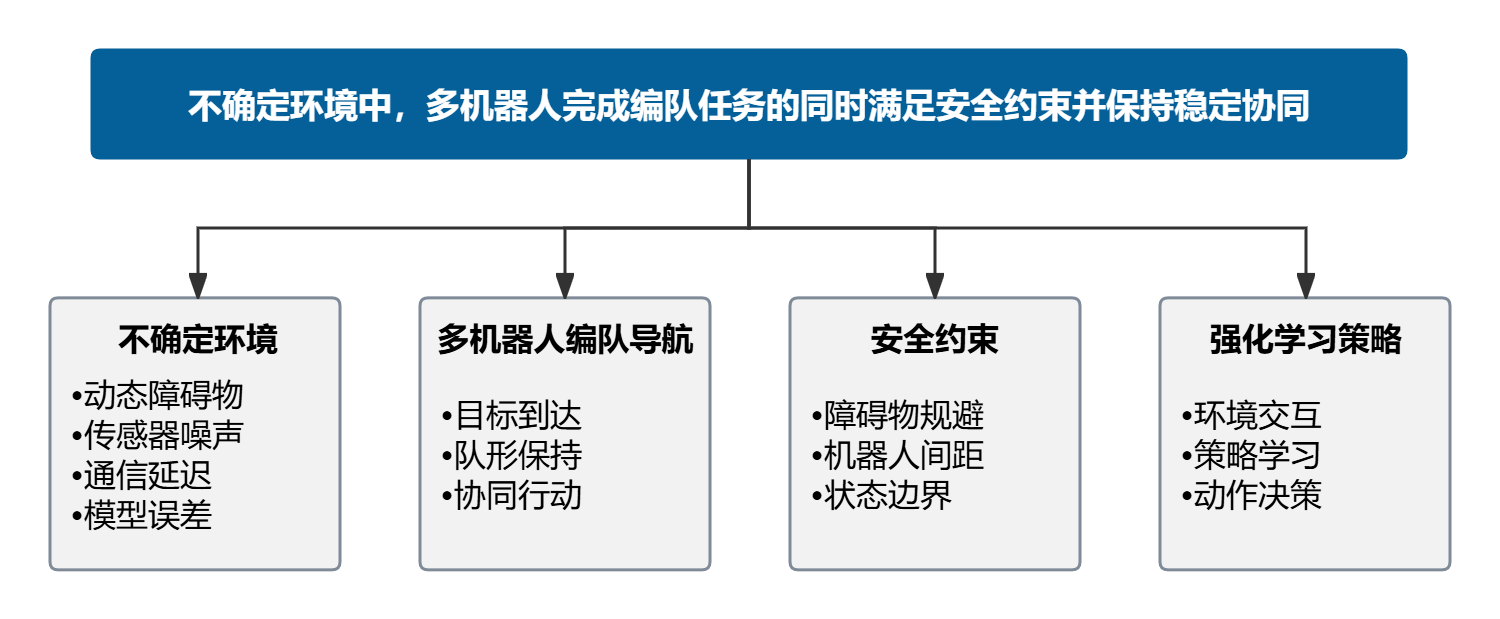
\includegraphics[width=0.8\textwidth]{images/background.png}
    \figcap{问题场景}{Problem scenario.}
    \label{fig:background}
\end{figure}

基于上述背景，本文围绕不确定环境下多机器人安全强化学习问题展开研究，重点关注三个方面：
一是利用约束流形与可达性分析对策略动作进行安全修正，减少训练和执行过程中的约束违背；
二是在多机器人编队导航任务中引入几何约束机制，使编队结构保持、安全距离约束和任务动作生成能够在统一框架下协同工作；
三是构建容器化仿真验证平台，为不同安全强化学习算法提供一致的运行环境和评估流程，从而验证所提方法在复杂场景中的有效性与可扩展性。

\section{研究意义}

多机器人系统在复杂环境中执行任务时，策略性能并不是唯一目标。对于编队导航这类任务而言，机器人既要到达目标区域，又要保持队形结构、避免碰撞，并在传感器噪声、障碍物变化和通信受限等条件下维持稳定运行。因此，如何在强化学习策略优化过程中同时处理任务收益和安全约束，是多机器人系统走向实际应用时必须面对的问题。本文围绕不确定环境下的多机器人安全强化学习展开研究，将约束流形、可达性分析、状态估计和几何约束机制引入策略学习过程，目的在于减少策略训练与执行中的约束违背，使学习得到的控制策略不仅具有较好的任务表现，也具备更稳定的安全边界。

在方法层面，本文把安全约束从奖励函数中的软惩罚移到了动作执行环节。多数安全强化学习方法用代价约束或拉格朗日乘子调节策略，其约束满足依赖超参数、且往往只在训练收敛后才较可靠，训练过程中仍可能违约；本文改用安全过滤、离线可达空间与奖励校准，把约束直接作用于动作的生成与修正，使不安全动作能在执行前被拦截。对编队导航中任务目标、安全距离与队形相互耦合的情形，几何约束策略学习进一步用几何关系而非奖励来修正策略输出，为提升多智能体方法的安全性与可解释性提供了一条区别于纯奖励塑形的途径。

在应用层面，仓储物流、灾害救援、巡检监测等场景中的多机器人往往要在动态环境下长时间运行，一次碰撞或队形失稳就可能中断任务甚至损坏设备，单纯追求任务效率并不够。本文实现的容器化仿真验证平台把运行依赖固化在镜像中，提供统一的算法接口与评估流程，缩小训练与部署环境之间的差异，也让不同算法能在相同条件下复现和比较，便于安全方法在进入实机前完成验证。

\section{研究内容}
本文研究不确定环境下的多机器人安全强化学习。与单纯的任务策略学习不同，这里的难点在于：训练阶段的试错探索本身就可能产生碰撞与队形破坏；而策略通常先在仿真中训练、再迁往实机，仿真与现实之间的动力学差异和传感器噪声又会削弱其可靠性。围绕这一难点，研究内容沿"安全动作约束—编队协同策略—系统验证平台"三条主线展开，力求在保证安全的前提下提升任务执行效率与部署可行性。技术路线如图~\ref{fig:tech_route}所示。

\begin{figure}[h]
    \centering
    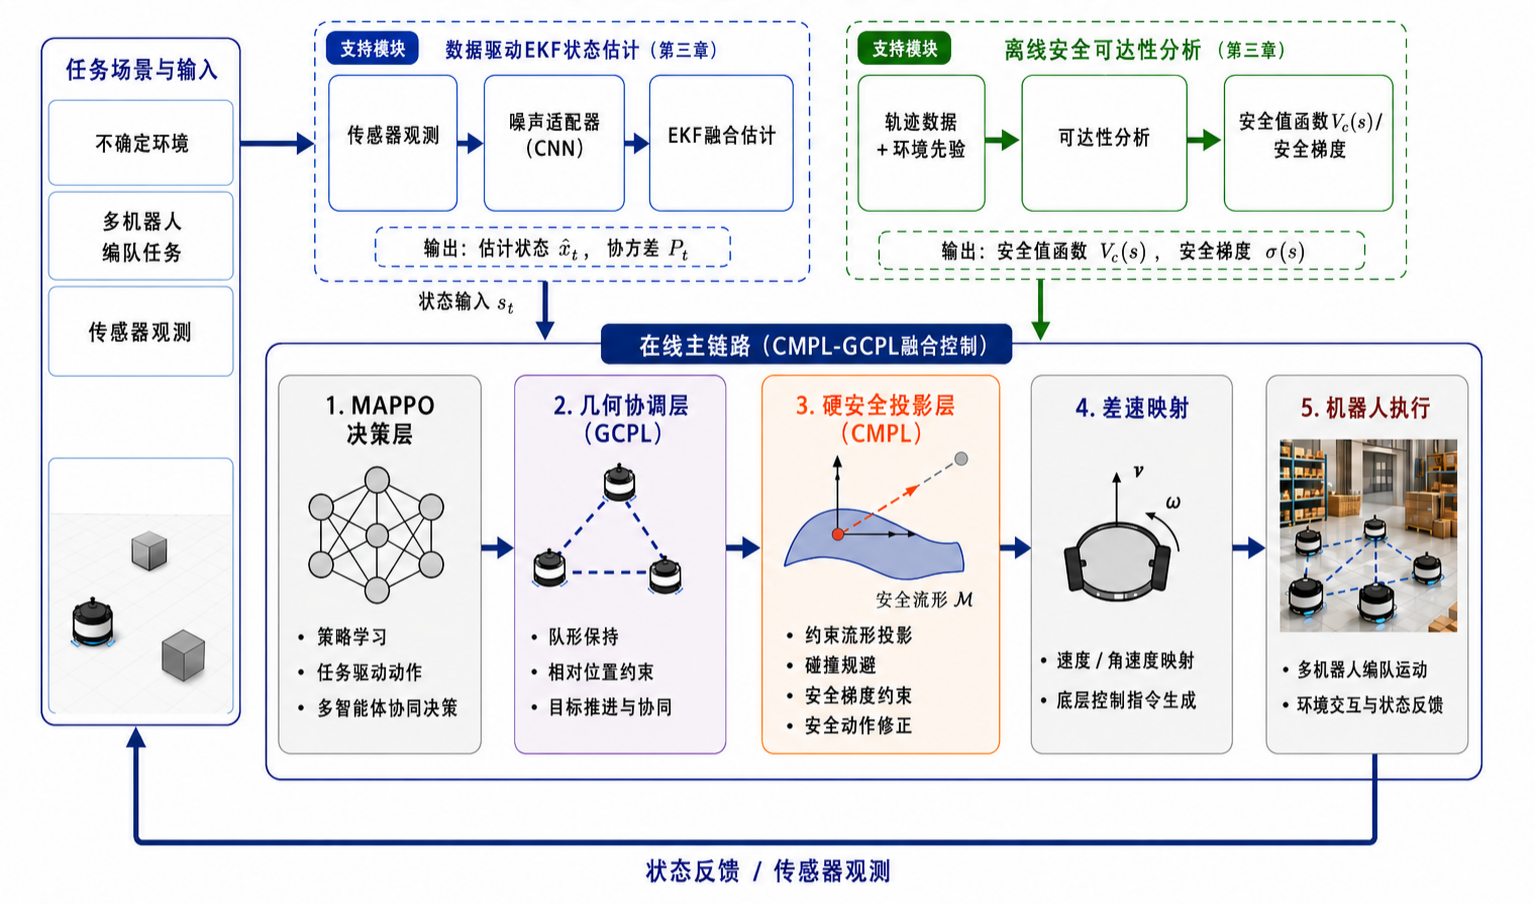
\includegraphics[width=0.8\textwidth]{images/tech_route.png}
    \figcap{技术路线}{Technical route.}
    \label{fig:tech_route}
\end{figure}


\textbf{（1）构建基于约束流形与可达性分析的安全策略修正方法}：传统强化学习算法主要通过与环境反复交互来最大化累积奖励，通常不会在动作生成阶段显式保证安全约束。已有安全强化学习方法虽然引入了代价约束或惩罚机制，但多数仍属于软约束形式，约束满足效果容易受到惩罚权重和训练状态的影响，在动态环境和感知噪声条件下难以稳定实现低违约甚至零违约表现。针对这一问题，本文引入约束流形思想，将机器人与障碍物之间的安全距离、状态边界等约束转化为增广状态空间中的流形约束，并通过零空间投影对策略输出的原始动作进行修正，使最终执行动作尽量保持原策略意图，同时满足安全可行条件。在此基础上，本文结合离线可达性分析，利用环境先验和采样轨迹构建安全可达空间，使安全裕度能够随机器人运动状态和环境风险变化进行调整。考虑到传感器噪声会影响安全判断的准确性，本文进一步引入数据驱动的状态估计模块，对速度相关噪声条件下的测量协方差进行自适应建模，从而为安全过滤器提供更可靠的状态输入。

\textbf{（2）提出面向多机器人编队导航的几何约束策略学习方法}：多机器人编队导航任务中，任务目标、安全约束和队形保持并不是彼此独立的要求。机器人在向目标移动时，需要根据邻近机器人和障碍物的位置不断调整自身动作；仅依赖奖励函数对队形偏差或碰撞风险进行惩罚，策略学习过程往往会出现收敛不稳定、局部行为不协调等问题。针对这一特点，本文在多智能体强化学习框架下构建基于几何约束的策略学习方法，以 MAPPO 生成任务驱动的动作，并在动作执行前引入几何过滤机制，对编队结构保持、机器人间安全距离和障碍物规避等约束进行统一处理。该方法利用约束流形和几何关系对策略输出进行修正，使多机器人系统在执行任务的同时维持较稳定的编队结构。

\textbf{（3）设计并实现多机器人安全强化学习的容器化仿真验证平台}：针对强化学习训练环境与部署环境的问题，本文设计并实现一套面向多机器人安全强化学习的容器化仿真验证平台。平台采用分层架构，通过容器化技术统一运行依赖，减少不同实验配置之间的环境差异。同时，平台提供标准化接口，并接入安全过滤器及多机器人协同策略。此外平台围绕安全性、任务性能、编队一致性和运行稳定性等指标构建评估流程，用于比较不同方法在相同场景下的表现。通过该平台，本文将前述安全约束机制与多机器人编队策略进行集成验证，从系统层面分析所提方法在复杂任务中的有效性、可扩展性和工程部署可行性。

\let\cleardoublepage\clearpage
\chapter{文献综述}
\section{安全强化学习研究现状}

在自动驾驶、服务机器人以及多机器人协同等真实应用场景中，安全性通常是系统能否部署的前提。机器人在运行过程中需要面对动态障碍物、传感器噪声、模型误差以及环境变化等不确定因素，即使策略在仿真环境中表现良好，进入真实系统后也可能因为状态估计偏差或外部扰动而产生不安全行为。因此，如何在策略学习和执行过程中持续保持安全约束，是机器人强化学习研究中长期存在的关键问题。

强化学习（Reinforcement Learning, RL）能够通过与环境交互学习控制策略，在处理复杂决策和自适应控制任务时具有一定优势~\cite{gu2024saferl_survey}。但这类方法通常依赖试错机制来改进策略，训练早期的探索行为并不稳定，在机器人系统中可能带来碰撞、越界或任务失败等风险。即使策略训练完成后具有较高回报，也不能直接说明其在整个学习过程或真实部署阶段始终满足安全要求。

在这一背景下，安全强化学习（Safe Reinforcement Learning, SafeRL）逐渐发展。该类方法通常将问题建模为约束马尔可夫决策过程（Constrained Markov Decision Process, CMDP）~\cite{altman1999cmdp}，在最大化期望回报的同时引入安全成本或状态约束。根据约束建模方式的不同，近期综述通常将相关方法划分为基于代价的方法和基于状态约束的方法~\cite{gu2024saferl_survey, liu2024safe_survey}。

\subsection{基于代价的方法}

基于代价的方法一般通过在优化目标中加入安全代价或惩罚项来约束策略行为。PID Lagrangian~\cite{stooke2020responsive}利用 PID 控制器调节拉格朗日乘子，使策略在奖励优化和成本约束之间进行动态平衡；IPO~\cite{liu2022ipo}采用对数屏障惩罚，将约束违背转化为优化过程中的内部惩罚；软屏障方法~\cite{wang2023soft_barrier}则从概率角度维持策略的可行性。这类方法通常不依赖特定机器人结构，具有较好的通用性，但其安全约束多属于软约束形式，实际违约率容易受到惩罚系数、乘子更新方式以及训练状态的影响，因此很难在所有阶段稳定实现零代价性能~\cite{liu2024safe_survey}。

在约束累积成本框架下，算法通常将碰撞次数或其他风险指标作为成本项，并为其设置上限。策略更新时，算法并不是直接禁止所有不安全动作，而是在收益和成本之间寻找折中解。因此，这类方法更适合任务性能与约束满足之间存在可接受权衡的场景。为了实现这一目标，相关研究常采用信赖域方法、内点法或拉格朗日松弛等约束优化技术，在策略改进过程中限制安全成本的增长。例如，CPO（Constrained Policy Optimization）~\cite{achiam2017constrained} 和 PCPO~\cite{yang2020projection} 通过引入信赖域约束，使策略更新幅度保持在安全成本允许的范围内；RCPO~\cite{tessler2018reward} 则将约束项转化为奖励函数中的惩罚项，并通过交替更新策略和乘子来逼近约束目标。除此之外，机会约束方法从概率角度限制智能体进入不安全状态的可能性，使风险发生概率低于预设阈值~\cite{ono2015chance, wang2023enforcing, chen2024probabilistic}。

总体来看，基于代价的方法已经形成了较为完整的研究体系，在不同任务和算法框架中均有较多应用。这类方法的安全性通常依赖对成本函数和惩罚参数的合理设定，约束满足也往往是统计意义或期望意义上的结果。当任务要求机器人在训练和执行过程中尽量避免任何碰撞或越界时，仅依靠代价惩罚并不足以提供严格保证。尤其在多机器人编队导航任务中，单个智能体的局部违约可能引发队形破坏或连锁碰撞，因此训练过程中的持续安全性仍然是这类方法需要进一步解决的问题。

\subsection{基于状态约束的方法}

与基于代价的方法不同，基于状态约束的方法更关注系统状态是否始终保持在安全集合内。该类方法通常通过限制动作空间或修正策略输出来避免系统进入危险状态。控制屏障函数（Control Barrier Functions, CBFs）~\cite{dawson2023safe_cbf, as2022cbfrl} 是其中较有代表性的一类方法，其核心思想是在控制输入层面对动作进行修正，使系统状态保持在前向不变的安全集内。CBF 能够提供较强的安全解释，但在复杂环境中构造合适的屏障函数并不容易，尤其当障碍物分布、动力学模型或观测条件发生变化时，屏障函数的设计和验证都会变得更加困难。Recovery RL~\cite{thananjeyan2021recovery} 则通过离线方式学习恢复区域，当智能体接近不安全边界时切换到恢复策略，从而降低进入危险状态的风险，但这种方法的安全效果很大程度上取决于恢复边界学习是否准确。

另一类研究通过约束状态可行性来间接限制策略行为。由于动作会引起状态转移，当策略选择的动作能够使系统始终停留在可行区域内，策略就可以被认为是安全的。部分研究采用时序逻辑对探索行为进行验证，以保证动作序列满足预设的安全规范~\cite{li2019temporal}；部分方法利用 Lyapunov 函数构造能量边界，将智能体动作限制在稳定区域内，避免系统演化到危险状态~\cite{chow2018lyapunov, chow2019lyapunov, koller2018learning}。这类方法通常需要对状态空间、动力学模型或约束形式作出明确假设，面对未知环境或复杂传感噪声时，泛化能力会受到限制。

高斯过程也被用于探索阶段的安全状态空间估计。相关方法通过建模环境不确定性，在策略探索过程中逐步扩展已验证的安全区域~\cite{turchetta2016safe, berkenkamp2015safe, sui2015safe, wachi2018safe}。例如，SafeMDP~\cite{turchetta2016safe} 使用高斯过程对环境进行建模，并借助置信区间评估状态安全性，使探索过程被限制在已经验证的安全状态范围内。\cite{berkenkamp2015safe} 则将高斯过程模型的在线更新嵌入鲁棒控制框架，通过数据驱动方式逐步减少系统不确定性，在保持稳定性的同时提升控制性能。此类方法能够较好地刻画不确定性，但在高维状态空间或多机器人场景中，计算开销和样本需求往往较高。

近年来，也有研究尝试使用约束流形构建安全空间，通过调整机器人动作使其沿约束允许的方向运动~\cite{liu2022robot}。这类方法将安全约束转化为几何结构，为动作修正提供了更直接的表达方式，但现有方法大多仍面向已知且相对固定的环境，面对动态障碍物、感知噪声和部分可观测条件时，其适用范围仍然有限。ATACOM~\cite{liu2022atacom, liu2023safe_manipulation} 进一步提出利用零空间投影将动作映射到约束流形的切空间，从而为机器人操作任务提供可证明的约束满足性。该方法为安全动作修正提供了清晰的几何解释，但它通常假设系统在每一时刻都能够获得精确状态信息和已知障碍物位置；在传感器噪声明显、环境信息不完整或多机器人协同约束不断变化的场景中，这一假设往往难以满足。因此，如何在保留约束流形安全修正优势的同时，引入状态估计、可达性分析和多机器人几何约束机制，仍然具有进一步研究的必要。

\section{多智能体强化学习研究现状}
在多智能体中，机器人不仅需要满足自身的安全约束并最大化回报，还需确保团队行为的整体安全性，平衡安全约束与奖励优化 \cite{chen2024duality}。
现有多智能体安全强化学习方法中，MACPO \cite{gu2023safe} 和 MAPPO-Lagrangian \cite{gu2023safe} 具有一定代表性。MACPO 在策略更新过程中引入信赖域思想，通过限制个体策略的更新幅度来降低安全成本突增的风险，并结合全局约束机制维持多智能体系统的整体安全性。
MAPPO-Lagrangian 则沿用 PPO 的裁剪目标进行策略优化，同时利用拉格朗日乘子对全局约束权重进行动态调节，使策略在任务回报和安全代价之间不断调整。此类方法为多智能体安全强化学习提供了较为直接的优化框架，也便于与现有策略梯度算法结合。
这类方法通常建立在较强的优化假设之上，尤其依赖原始问题与对偶问题之间具有较好的对应关系。
在多智能体系统中，不同智能体策略相互影响，个体策略与联合行为占用度量之间往往呈现非凸关系，强对偶性难以始终成立。
当存在非零对偶间隙时，对偶问题就不能完全刻画原始约束优化问题，拉格朗日乘子得到的解也可能与原始问题的最优解不一致，甚至出现约束满足和任务性能同时难以稳定收敛的情况。
对于多机器人编队导航这类约束耦合较强的任务，仅依赖全局代价或乘子调节往往不足以精细描述机器人间距、队形保持和避障安全等几何关系，
因此仍有必要在策略学习过程中引入更直接的安全约束表达与动作修正机制。
% 本文在此流形投影范式基础上进行了三方面扩展：（i）通过离线可达性分析利用先验地图预计算环境相关安全裕度，替代实时障碍物检测与跟踪；（ii）引入数据驱动 EKF 提升噪声条件下的状态估计鲁棒性；（iii）通过奖励校准机制引导策略学习安全行为，无需外部惩罚调参。

\subsection{多智能体编队研究现状}

近年来，无人系统在巡检、救援、运输和协同作业等场景中的应用不断扩展，多智能体编队控制也因此受到较多关注。编队控制通常要求多个智能体在运动过程中形成并维持特定空间结构，同时完成目标到达、避障和协同行动等任务。已有综述将编队控制方法概括为领航-跟随（leader-follower）\cite{sui2020formation}、虚拟结构（virtual structures）\cite{yan2021formation} 和基于行为的方法（behavior-based approaches） \cite{liu2018survey}。

领航-跟随方法结构简单，便于实现，但对领航者依赖较强，一旦领航者失效，编队任务容易受到影响。虚拟结构方法将编队视为整体结构进行控制，能够保持较稳定的队形，但在队形调整和复杂环境适应方面灵活性不足。相比之下，基于行为的方法 \cite{xu2014behavior, quan2023robust} 更强调机器人根据局部观测动态调整动作，适合处理目标到达、队形保持和避障等多重要求。随着多智能体强化学习的发展，MARL 已逐渐用于编队控制任务，并取得了一定成果 \cite{sui2020formation,yan2022relative,khan2020graph}。

现有强化学习编队方法中，PPO 及其多智能体扩展应用较为广泛。文献 \cite{sadhukhan2022proximal} 将 PPO 与课程学习结合，通过机器人之间的夹角信息维持编队形状；文献 \cite{yan2022relative} 采用 MAPPO，并结合课程学习、参考目标和相对位置信息实现编队控制。针对四旋翼编队，文献 \cite{batra2022decentralized} 基于 PPO 引入注意力机制，对相邻四旋翼状态进行编码，以减少碰撞并提升飞行性能，其思想与文献 \cite{hoshen2017vain, chen2019crowd} 中的注意力建模方法相关。文献 \cite{wang2019pattern} 则在集中训练、分散执行（Centralized Training with Decentralized Execution, CTDE）框架下，利用 PPO 实现移动机器人的静态编队控制。

除 PPO 类方法外，其他强化学习框架也被用于编队控制。文献 \cite{sui2020formation} 将模仿学习与强化学习结合，在领航-跟随框架下构建分布式编队控制器。文献 \cite{khan2020graph} 将策略梯度方法与图卷积网络（Graph Convolutional Network, GCN）结合，用于无人机静态编队控制。文献 \cite{xie2021reinforcement} 和文献 \cite{zhou2019learn} 分别基于深度确定性策略梯度（Deep Deterministic Policy Gradient, DDPG）和深度 Q 网络（Deep Q-Network, DQN），实现了海上无人艇的领航--跟随编队控制。

总体来看，现有研究已证明强化学习方法在多智能体编队控制中的可行性，但多数工作更关注队形形成和任务完成效果，对安全距离、障碍物规避以及训练过程中的约束违背考虑仍不充分。在复杂环境下，仅依赖奖励函数引导编队行为，难以保证策略输出始终满足安全要求。因此，将几何约束、安全过滤和动作修正机制引入多智能体策略学习，仍具有进一步研究价值。

\subsection{多智能体安全强化学习}
在编队控制下，安全性意味着在训练与执行过程中避免任何形式的碰撞。

MARL 的核心目标是在多种交互场景（包括协作、竞争及混合环境）中协调多个智能体之间的行为。
安全多智能体强化学习（Safe MARL）近年来已成为研究热点之一 \cite{garg2024learning}。

文献 \cite{cai2021safe} 将 CBF 与多智能体深度确定性策略梯度（MADDPG）\cite{lowe2017multi} 相结合，实现了两智能体在导航过程中无碰撞运动，其中 CBF 通过构造满足安全约束的控制律来保证系统安全。文献 \cite{zhang2023spatial} 研究了注意力模块与基于 CBF 的分布式安全屏蔽机制在多自动驾驶车辆场景中降低碰撞率的有效性。

不同于上述方法，文献 \cite{sheebaelhamd2021safe} 在 MADDPG 框架中引入训练得到的集中式神经网络作为安全层，并在协作导航任务中显著降低了碰撞发生率。文献 \cite{elsayed2021safe} 则基于确定性有限自动机（Deterministic Finite Automaton, DFA）提出了集中式与分布式相结合的安全屏蔽策略，以确保协作导航任务中的智能体安全，其中 DFA 通过定义有限状态集合来刻画安全约束。

文献 \cite{zhang2019mamps} 提出了一种预测式安全屏蔽方法，并与 MADDPG 相结合以保证多智能体协作导航的安全性，并在简化的多智能体粒子环境 \cite{mordatch2018emergence} 中验证了其有效性。

基于行为的编队控制问题中，由于机器人需要在空间上保持紧密相对位置，碰撞风险比传统协作导航场景更高。已有研究多集中于协作导航任务，该类任务通常可通过训练单一策略并部署至多个机器人来实现 \cite{everett2021collision, brito2021go, vinod2022safe}。然而，行为驱动的编队控制需要机器人在训练过程中持续交互，因此更适合采用多智能体强化学习方法。文献 \cite{zhang2022barrier} 利用基于强化学习的模型预测控制方法，在保证安全的前提下实现了移动机器人的领航–跟随编队控制。该方法通过为每个机器人设定目标位置来维持编队结构。

\section{Hamilton–Jacobi 可达性分析}

Hamilton–Jacobi（HJ）可达性分析~\cite{bansal2017hj_reachability}通过求解 HJ 变分不等式（HJ-VI）计算反向可达管（Backward Reachable Tubes, BRTs），从而基于受控不变集提供形式化的安全保证。近期研究致力于提升其可扩展性：例如基于神经网络的近似方法~\cite{hsu2021safety, so2023rtreach}能够在更高维空间中进行可达性计算。然而，大多数方法仍需在线计算或依赖环境动力学模型。本文则采用离线、数据驱动的方式：将 HJ-VI 离散化为可行性 Bellman 算子，并利用期望分位回归~\cite{kostrikov2022iql}从采集轨迹数据中求解，从而在无需显式动力学模型的情况下近似 BRT 值函数。结合静态障碍物先验地图，该方法实现了安全裕度计算与部署阶段的解耦，适用于资源受限的机器人平台。

% \subsection{多任务几何约束融合}
% 为解决多任务几何约束融合问题，RMPflow 提出了一种基于黎曼几何的运动策略组合框架。RMPflow 将每个任务空间中的控制策略表示为 Riemannian Motion Policy (RMP)，并通过雅可比映射在不同空间之间进行一致变换与组合，从而实现多个任务策略的解析融合~\cite{cheng2018rmp}。

% RMPflow 已被应用于机械臂操作、移动机器人导航以及人机协作等场景，在复杂约束环境中展现出良好的稳定性与鲁棒性~\cite{cheng2018rmp, li2021rmp2}。然而，该方法通常依赖于精确系统模型与人工设计的任务策略，其在高度不确定环境中的适应能力有限。此外，RMPflow 本身属于模型驱动方法，缺乏从交互数据中学习高层决策策略的能力，这在多机器人协同探索与动态环境任务中成为主要限制。

% 近年来，研究者开始探索将强化学习与几何约束控制相结合的框架，以同时获得学习方法的适应性与几何控制的稳定性。例如，通过在强化学习策略外层叠加几何安全控制器，或采用分层控制结构，使高层策略负责任务决策，而低层控制器保证运动学与动力学约束的满足~\cite{deisenroth2013gaussian,}. 这种融合方法被认为是实现复杂环境中安全多机器人协作的重要方向。

% 本文提出将 RMPflow 与强化学习进行分层融合，在保证几何安全约束的同时提升多机器人协作策略的环境适应能力。


% 黎曼运动策略（Riemannian Motion Policies，简称 RMPs）是一种定义在流形上的策略的数学表示方法，而 RMPflow 是一种用于组合多个 RMP 的递归算法。

% 一个机器人或一组机器人，其配置空间 C 是一个光滑的 d 维流形。假设 C 存在一个全局的广义坐标 $q : C \to \mathbb{R}^d$ ，系统可以通过反馈线性化，使其可以直接通过广义加速度进行控制，即 $\ddot{q} = u(q, \dot{q})$。我们称 u 为策略或控制器，$(q, \dot{q})$为系统状态。

% RMPflow  将一个任务拆解为一系列子任务，例如避开障碍物、到达目标、跟踪轨迹等，即任务空间 T 由多个子任务空间组成的集合，每个空间对应一个子任务。假设任务空间 T 与配置空间 C 可以通过一个平滑的任务映射 $\psi : C \to T$ 相互关联。RMPflow 的目标是在配置空间 C 中生成控制策略 u，使得机器人在任务空间 T 中做出期望的行为。

% \section{黎曼运动策略（RMPs）}
% 黎曼运动策略（Riemannian Motion Policies, RMPs） 是一种定义在流形上的控制策略表示方法。设 $\mathcal{M}$ 是一个维度为 m 的流形，其广义坐标为 $x \in \mathbb{R}^m$。RMP 在流形 $\mathcal{M}$ 上可以通过标准形式和自然形式两种形式进行表示。

% RMP 的标准形式表示为一对 $(a, M)^{\mathcal{M}}$，其中：$a : (x, \dot{x}) \mapsto a(x, \dot{x}) \in \mathbb{R}^m$ 是期望加速度（即控制输入）；$M : (x, \dot{x}) \mapsto M(x, \dot{x}) \in \mathbb{R}^{m \times m}_+$ 是惯性矩阵（或权重矩阵），用于在与其他 RMP 合并时表示该策略的重要性。

% 根据标准形式，我们可以得到 RMP 的自然形式，表示为一对 $[f, M]^{\mathcal{M}}$，其中 $f = M a$ 是期望力。引入自然形式主要是出于计算上的便利。

% 在流形 $\mathcal{M}$ 上的 RMP 通常来自一类称为几何动力系统（Geometric Dynamical Systems，GDSs） 的系统。GDS 是经典的简单机械系统（Simple Mechanical Systems, SMSs）的一种推广。在 GDS 中，动能度量 G 是配置和速度的函数，即 $G(x, \dot{x}) \in \mathbb{R}^{m \times m}_+$。这意味着动能可以依赖于运动方向，这在避障等应用中是有用的。GDS 的动力学形式如下：
% \begin{equation}
%     (G(x, \dot{x}) + \Xi_G(x, \dot{x})) \ddot{x} + \xi_G(x, \dot{x}) = -\nabla_x \Phi(x) - B(x, \dot{x}) \dot{x} 
% \end{equation}
% 其中：$B : \mathbb{R}^m \times \mathbb{R}^m \to \mathbb{R}^{m \times m}_+$ 是阻尼矩阵；$\Phi : \mathbb{R}^m \to \mathbb{R}$ 是势函数；曲率项 $\Xi_G$ 和 $\xi_G$ 由度量 G 所诱导，具体表达为：
% \begin{equation}
% \begin{aligned}
%     \Xi_G(x,\dot{x}) &:= \frac{1}{2} \sum_{i=1}^{m} \dot{x}_i, \partial_{\dot{x}} g_i(x, \dot{x}) \\
%     xi_G(x, \dot{x}) &:= \partial_x G(x, \dot{x}) \dot{x} - \frac{1}{2} \nabla_x ( \dot{x}^\top G(x, \dot{x}) \dot{x} )
% \end{aligned}
% \end{equation}
% 其中：$g_i$ 表示 G 的第 i 列；$x_i$ 表示 x 的第 i 个分量；$\partial_x G(x, \dot{x}) \dot{x} = [\partial_x g_i(x, \dot{x}) \dot{x}]_{i=1}^m$，即将各列拼接为矩阵。

% 给定上述 GDS 动力学，我们可以自然地构造出对应的 RMP：其标准形式为：$a = \ddot{x}, \quad M(x, \dot{x}) = G(x, \dot{x}) + \Xi_G(x, \dot{x})$因此，速度相关的度量 G 在与其他 RMP 合并时，提供了一个速度相关的重要性权重 M。

% \section{ RMPflow}

% RMPflow  是一种用于在构型空间上生成控制策略的算法，它依赖于各个子任务的 RMP（例如避障、到达目标点等）。给定机器人在构型空间中的状态信息，以及针对各个子任务独立设计的控制器（即 RMPs），RMPflow 通过组合这些控制器，在构型空间上生成控制输入。RMPflow 引入了以下两个关键结构： 
% \begin{itemize}
%     \item 一种数据结构：RMP 树（RMP-tree），用于描述任务映射 ψ 的结构； 
%     \item 一组算子：RMP 代数（RMP-algebra），用于在 RMP 树中传播信息。
% \end{itemize}

% RMP 树是一个有向树。树中每个节点 u 都关联一个定义在流形 $\mathcal{M}$ 上的状态 $(x, \dot{x})$，以及一个 RMP $(f_u, M_u)^{\mathcal{M}}$。每条边 e 则带有一个从父节点到子节点的光滑映射 $\Psi_e$。例如，如图~\ref{fig:rmp树}所示的是一个典型的 RMP 树。树的根节点 r 对应机器人在构型空间中的状态$(q, \dot{q})$，以及该空间上的控制策略 $(f_r, M_r)^C$。每个叶节点$l_k$表示一个子任务，其控制策略为定义在子任务空间 $T_k$上的 RMP $(f_{l_k}, M_{l_k})^{T_k}$。
% \begin{figure}
%     \centering
%     
\includegraphics[width=1\linewidth]{硕士毕业论文/毕业论文-safeMARL/images/rmp.png}
%     \caption{RMP树示例}
%     \label{fig:rmp树}
% \end{figure}
% RMP代数 包括三个基本操作符：前向传播（pushforward）、反向传播（pullback） 和解析（resolve）。具体作用过程如下：
% 设某节点 u 有 N 个子节点，分别记为 ${v_j}_{j=1}^N$，边记为 ${e_j}_{j=1}^N$，如图~\ref{fig:rmp树}所示。假设 u 所在流形为 M，每个子节点 $v_j $所在流形为 $N_j$，则各个操作符作用如下：
% 前向传播将状态从父节点 u 传播到其子节点 ${v_j}_{j=1}^N$。 给定 u 的状态 $(x, \dot{x})$，对于每个子节点 $v_j$，通过映射 $\psi_{e_j}$ 计算其状态为：
% \begin{equation}
%     (y_j, \dot{y}_j) = (\psi_{e_j}(x), J_{e_j}(x) \dot{x})
% \end{equation}
% 其中 $J_{e_j} = \frac{\partial \psi_{e_j}}{\partial x}$ 是映射 $\psi_{e_j}$ 的雅可比矩阵。

% 反向传播将子节点${v_j}_{j=1}^N$的 RMP 聚合为父节点 u 的 RMP。给定每个子节点的 RMP $(f_{v_j}, M_{v_j})^{N_j}$，父节点的 RMP $(f_u, M_u)^M$ 计算如下：
% \begin{equation}
%     f_u = \sum_{j=1}^{N} J_{e_j}^T (f_{v_j} - M_{v_j} \dot{J}_{e_j} \dot{x}), \quad M_u = \sum_{j=1}^{N} J_{e_j}^T M_{v_j} J_{e_j}
% \end{equation}

% 解析操作将自然形式（natural form）的 RMP 转换为标准形式（canonical form）。 给定自然形式 RMP $(f_u, M_u)^M$，标准形式为：$(a_u, M_u)^M, \quad a_u = M_u^{\dagger} f_u$其中 $\dagger$ 表示 Moore-Penrose 伪逆。

% 在 RMP 树结构确定之后，RMPflow 会按照前向传播、叶节点评估、反向传播以及解析输出的计算流程生成最终控制策略，具体过程如下：

% 在前向传播阶段，系统以根节点为起点，将当前机器人的状态沿任务树逐层向下传递，该过程通过递归方式完成。pushforward 操作将配置空间中的位姿与速度映射到各个任务空间，使不同层级的节点都能够获得与自身相关的状态信息。由于叶节点通常定义在不同的空间中，或者描述距离关系，或者描述相对位姿，或者直接与目标位置相关，因此需要借助雅可比矩阵进行变量变换，将全局状态转换为各任务所需的局部变量及其变化率，使各叶节点能够在各自坐标系下进行计算。

% 在叶节点评估阶段，系统根据节点所对应的任务目标构造自然形式的 RMP $(f_{l_k}, M_{l_k})$。该形式一般由几何动力系统给出，在任务空间内通过势函数与阻尼项刻画系统的演化趋势，从而生成具有物理意义的广义力 $f_{l_k}$ 与度量矩阵 $M_{l_k}$。广义力反映任务期望的加速度方向，而度量矩阵描述任务在当前状态下的作用强度及方向权重。当机器人接近约束边界时，与安全相关的任务度量会增大，使其在后续融合中占据更高权重；而用于引导系统接近目标的任务，其度量变化相对平缓。

% 在反向传播过程中，系统从所有叶节点出发，通过 pullback 操作将自然形式的 RMP 逐层上传至父节点，并在传递过程中完成合并。不同任务空间中得到的广义力与度量矩阵被统一映射回根节点所在的配置空间，并依据各自的度量进行加权叠加。该过程保证各任务在几何上的一致性，使其能够在同一坐标框架下融合。当某一任务的度量值较大时，其在合成结果中的影响随之增强，而其他任务的作用相对减弱。

% 当所有叶节点的信息回传至根节点后，系统对汇总得到的自然形式 $(f_r, M_r)$ 进行解析，将其转换为可直接用于控制的标准形式。具体做法是求解加权最小二乘意义下的最优加速度：
% \begin{equation}
% a_r = M_r^{\dagger} f_r
% \end{equation}

% 该求解过程等价于在统一的黎曼度量下寻找整体上最符合各项任务约束的加速度解。与基于硬优先级的传统控制方式相比，该方法依赖度量矩阵连续调节各任务的影响程度，使权重变化保持平滑，从而减小任务切换带来的突变与振荡。

% 在执行阶段，机器人按照 $\ddot q = u = a_r$ 的形式施加控制输入。对于移动机器人系统，配置空间中的加速度还需进一步映射为底层驱动可执行的速度或角速度指令，经此转换后控制量才能作用于执行机构。通过上述流程，系统能够在多任务与多约束条件下持续生成平滑且稳定的控制指令，并在满足物理约束的前提下协调各类控制目标。

\section{本章小结}

本章系统梳理了安全强化学习、多智能体强化学习与多机器人编队控制的研究进展。现有安全强化学习方法主要分为基于代价约束与基于状态约束两类：
前者具有通用性但通常难以实现严格零违约，后者能够提供更强的安全保证，
但常依赖精确状态估计、在线环境感知及较强模型假设。在多智能体场景中，现有方法虽在约束优化方面取得进展，
但仍面临强对偶性难以满足、策略协同复杂度高以及训练过程安全性不足等问题。

针对上述不足，本章进一步分析了编队任务中“结构保持 + 避障安全 + 目标到达”的耦合挑战，
并综述了 Hamilton--Jacobi 可达性分析在形式化安全保证方面的优势及其计算代价问题。
基于此，本文后续章节将以安全可达空间为先验约束基础，结合约束流形动作修正与数据驱动状态估计，
构建兼顾安全性、可部署性与协同性能的多智能体安全强化学习方法。
\chapter{不确定环境下安全约束方法}

在不确定环境中，机器人自主决策不仅需要完成目标导航、避障或任务执行等基本功能，还需要在感知误差和环境变化等因素影响下保持稳定的安全行为。
传统强化学习方法通常通过奖励惩罚引导策略避免危险状态，但这类软约束方式难以保证训练与部署过程中始终满足硬安全约束；
同时，机器人系统的运动学限制和状态估计误差也会进一步放大策略执行中的碰撞风险。

针对上述问题，本章围绕不确定环境下的安全强化学习展开研究，提出一种基于约束流形的安全策略学习方法。
该方法将安全约束显式嵌入策略执行过程，通过约束流形投影对策略动作进行实时修正，并结合离线安全可达性分析与数据驱动状态估计机制，提高策略在复杂环境中的安全性和鲁棒性。

% 针对机器人在强安全约束环境中进行强化学习训练时须严格遵循硬安全约束的问题，
% 同时优化感知不确定性以及安全约束高度依赖先验模型的问题，本文提出了一种基于约束流形的安全空间过滤框架。
% 利用系统可达性分析为，从离线轨迹数据中预先计算环境感知的安全区域，
% 在部署阶段无需实时感知即可自适应调节安全裕度，从而为机器人提供具有物理意义的安全边界描述。
% 同时引入流形安全过滤与校准机制，通过零空间投影（Null-space Projection）将策略动作投影至约束流形的切空间上，
% 并结合奖励校准机制引导策略学习内在的安全行为，使得策略更新始终满足硬安全约束要求。
% 针对实际机器人系统中普遍存在的传感器噪声与定位误差问题，本文进一步引入数据驱动的扩展卡尔曼滤波（EKF），
% 利用卷积神经网络（CNN）学习噪声参数，使测量协方差能够适应与速度相关的传感器噪声，
% 对机器人自身状态进行更加精确和鲁棒的估计，从而显著降低了因感知不确定性引发的安全风险。
\section{问题定义}
为刻画机器人安全导航中的安全关系，考虑一个机器人在包含 $n$ 个障碍物的复杂环境中进行导航任务。令 $s_t = [p_t^\top, v_t^\top]^\top \in \mathcal{S} \subseteq \mathbb{R}^d$ 表示机器人在离散时间步 $t$ 时的状态，其中 $p_t \in \mathbb{R}^{d_p}$ 代表位置向量，$v_t \in \mathbb{R}^{d_p}$ 代表速度向量（$d_p$ 通常为 2 或 3）。为了定量描述安全，引入基于距离的约束函数。安全性的核心要求是机器人与环境中任何障碍物之间必须保持一定的物理间隔。定义约束集合如下：$$c_i(s_t) := d_{\text{safe}} - \|p_t - o_i\|_2 \leq 0, \quad \forall i \in \{1, \ldots, n\}$$其中，$d_{\text{safe}} > 0$ 表示预设的最小安全距离阈值，$o_i \in \mathbb{R}^{d_p}$ 为第 $i$ 个障碍物在空间中的坐标，$\|\cdot\|_2$ 为欧几里得范数。

若状态 $s_t$ 满足对所有 $i$ 均有 $c_i(s_t) \leq 0$，则称该状态是安全的。在物理上意味着机器人的中心与所有障碍物的中心的距离均大于等于 $d_{\text{safe}}$。在实际应用中，该距离通常考虑了机器人自身的几何半径以及感知系统的不确定性冗余。

在强化学习（RL）框架下，将安全导航任务建模为一个约束马尔可夫决策过程（CMDP），记为六元组 $(\mathcal{S}, \mathcal{A}, P, R, \gamma, C)$。其中：$\mathcal{S}$ 和 $\mathcal{A}$ 分别为状态空间和动作空间；$P: \mathcal{S} \times \mathcal{A} \times \mathcal{S} \rightarrow [0, 1]$ 为环境的状态转移概率核；$R: \mathcal{S} \times \mathcal{A} \rightarrow \mathbb{R}$ 为奖励函数，鼓励机器人靠近目标点；$\gamma \in [0, 1)$ 为折扣因子；$C = \{c_i: \mathcal{S} \rightarrow \mathbb{R}\}_{i=1}^k$ 为与环境障碍物对应的约束集合。在具有 $k=n$ 个硬约束（每个障碍物对应一个约束）的设置下，安全强化学习的目标是寻找到一个最优策略 $\pi: \mathcal{S} \rightarrow \mathcal{A}$，使得在满足所有时间步的硬安全约束前提下，最大化累积期望回报：$$\max_{\pi} \mathbb{E}_{\pi}\left[ \sum_{t=0}^{T} \gamma^t R(s_t, a_t) \right]$$$$\text{s.t. } c_i(s_t) \leq 0, \quad \forall t \in \{0, \dots, T\}, \forall i \in \{1, \dots, n\}$$与传统的强化学习不同，CMDP 要求算法在探索过程中不仅要学习任务技能，还必须严格遵守状态空间的边界，避免任何形式的碰撞。

此外，考虑到机器人系统（如差速驱动轮式机器人或无人机）普遍存在非完整约束（Nonholonomic Constraints），不能简单地假设状态可以任意改变。因此，本文将机器人的底层运动学建模为连续时间的控制仿射系统（Control-Affine System）：$$\dot{s} = f(s) + G(s) a$$

在该模型中：$a \in \mathcal{A} \subseteq \mathbb{R}^m$ 是 $m$ 维控制控制量（如推力、转矩或速度指令）；$f(s): \mathcal{S} \rightarrow \mathbb{R}^d$ 称为漂移项（Drift term），代表系统在无控制输入时的固有动力学演化；$G(s): \mathcal{S} \rightarrow \mathbb{R}^{d \times m}$ 为控制输入矩阵，定义了控制动作如何映射到状态的变化率上。动力学特例：质点模型（Single-Integrator）： 若 $f(s) = 0$ 且 $G(s) = I$，系统简化为全向移动模型。差速驱动模型： $G(s)$ 包含三角函数项（如 $\cos\theta, \sin\theta$），用以体现机器人朝向与运动速度之间的耦合关系。通过结合上述动力学模型与 CMDP 框架，本文的研究重点在于如何在复杂的动力学约束下，保证机器人在轨迹执行过程中的实时安全性。

\section{约束流形策略学习方法}
本文构建了一种面向安全强化学习的约束流形策略方法（Constrained Manifold Policy Learning，CMPL），通过约束流形建模、可达性分析与状态估计的协同设计，实现策略安全性。整体框架由以下三个核心模块组成：
\begin{itemize}
\item \textbf{基于约束流形的安全过滤器}：
针对策略输出可能违反安全约束的问题，本文设计基于零空间投影的动作修正机制，将名义动作投影至约束流形的切空间，从而保证生成动作始终满足硬约束。在此基础上，引入动态奖励校准机制，对动作修正幅度进行显式调节，使策略在训练过程中逐步适应约束结构，形成内生的安全行为，而非单纯依赖外部惩罚项。

\item \textbf{离线安全可达空间构建}：  
为提升系统对环境约束的感知能力，本文引入可达性分析方法，在离线阶段基于采样轨迹与环境先验信息预计算安全可达区域。所得可行性值函数在部署时用于动态调节安全裕度，使系统在无需实时精确建模障碍物的情况下，仍能保持保守且稳定的安全行为。

\item \textbf{数据驱动的状态估计模块}：  
为缓解感知噪声对安全决策的影响，本文构建基于数据驱动的扩展卡尔曼滤波（EKF）框架，通过卷积神经网络学习观测噪声参数，使测量协方差能够随运动状态自适应调整，从而在速度相关噪声条件下维持较高的状态估计精度，保证安全过滤器输入的可靠性。
\end{itemize}

在具体实现中，可达性分析与状态估计模块均采用离线构建方式。前者利用环境数据提前学习安全裕度分布，后者根据交互数据刻画传感器噪声随运动状态变化的特征。部署阶段，系统只需调用已经得到的安全边界和噪声估计结果，无需重新进行在线训练或复杂优化。这样的设计降低了运行时计算开销，也提高了方法在资源受限机器人平台上的部署可行性。

\begin{figure}
    \centering
    
\includegraphics[width=1\linewidth]{images/framework.png}
    \caption{约束流形策略学习方法框架}
    \label{fig:placeholder}
\end{figure}
\subsection{约束流形投影}
流形是一个局部与欧几里得空间同胚的拓扑空间， 可以用于描述复杂的几何对象，例如曲线、曲面以及更高维的结构。约束流形是由某些约束条件定义的流形，这些约束条件限制系统的状态或行为。在几何上，这些约束可以用方程或不等式来描述。
\subsubsection{（1）松弛变量}
然而，不等式约束在优化和控制律设计中往往难以直接处理，且难以定义稳定的切空间（Tangent Space）。为此，本研究引入非负松弛变量（Slack Variables） $\mu \in \mathbb{R}^k_{\geq 0}$。通过将原始约束函数与松弛变量结合，可以将不等式约束转化为严格的等式约束形式：
\begin{equation}
    \bar{c}(s, \mu) := c(s) + \mu = 0, \quad \text{其中 } \mu \geq 0\label{eq:slack}
\end{equation}

引入松弛变量后，由于 $\mu$ 被限制为非负，任何满足等式 $\bar{c}(s, \mu) = 0$ 的点都必然满足 $c(s) = -\mu \leq 0$，安全性得到了自然的保证。这种转化允许将安全状态的搜索范围从一个区域（区域约束）缩小到一个精确定义的数学流形上。基于此，本文定义约束流形 $\mathcal{M}$ 为满足所有安全准则的状态集合：
\begin{equation}
    \mathcal{M} := { (s, \mu) \in \mathcal{D} \mid \bar{c}(s, \mu) = 0 
}\end{equation}

其中 $\mathcal{D} = \mathcal{S} \times \mathbb{R}^k_{\geq 0}$ 代表由原始状态与松弛变量构成的增广状态空间（Augmented State Space）。

\subsubsection{（2）零空间投影}
设$a_{\text{unsafe}} \in \mathbb{R}^m$表示由强化学习策略输出的未受约束的动作（unconstrained action）。
为了保证系统在执行控制输入时始终满足安全约束，安全过滤器首先在内部构造一个增广参考向量：
$u_{\text{ref}} =
\begin{bmatrix}
a_{\text{unsafe}}^\top , \mathbf{0}^\top
\end{bmatrix}^\top
\in \mathbb{R}^{m+k}$
其中 $k$ 表示约束数量（对应引入的松弛变量）。安全过滤器随后将该参考向量转换为满足所有约束条件的安全控制量：
$\begin{bmatrix}
a_{\text{safe}}^\top , \dot{\mu}^\top
\end{bmatrix}^\top$
其中 $a_{\text{safe}}$ 为最终执行的安全动作，$\dot{\mu}$ 为松弛变量的变化率。通过这种方式，可以在尽量保持策略原始控制意图的同时，保证系统始终处于安全可行域内。

对约束函数取时间导数可得：
\begin{equation}
\frac{d}{dt} \bar{c}(s, \mu) = J_s \dot{s} + J_\mu \dot{\mu} = J_s f(s) + J_c
\begin{bmatrix}
a \
\dot{\mu}
\end{bmatrix}
\label{eq:constraint_deriv}
\end{equation}

其中
$J_s = \frac{\partial \bar{c}}{\partial s},\quad
J_\mu = \frac{\partial \bar{c}}{\partial \mu}$
分别表示约束函数关于状态变量和松弛变量的雅可比矩阵。定义组合约束雅可比矩阵$J_c = [J_s G(s), J_\mu] \in \mathbb{R}^{k \times (m+k)}$ 刻画了控制输入与松弛变量对约束变化率的整体影响。

为了使系统状态始终保持在约束流形上，需要满足$\frac{d}{dt}\bar{c} = 0$ ，即系统的状态变化始终位于约束流形的切空间中。设 $J_c^\dagger$为为矩阵 $J_c$ 的 Moore--Penrose 伪逆，定义零空间投影算子：
\begin{equation}
N_c = I - J_c^\dagger J_c
\end{equation}

该投影矩阵将任意向量投影到 $J_c$ 的零空间，从而保证控制输入不会破坏约束条件。
则安全动作通过以下公式计算：
\begin{equation}
\begin{bmatrix}
a_{\text{safe}} \
\dot{\mu}
\end{bmatrix}
=
N_c u_{\text{ref}}
-
J_c^\dagger
\bigl(
J_s f(s) + K_c \bar{c}(s, \mu)
\bigr)
\label{eq:safe_action}
\end{equation}

其中 $K_c > 0$ 为约束修正增益。公式中的第一项将增广参考向量投影到约束零空间（即约束流形的切空间），从而保证生成的控制输入不会导致约束违反；第二项同时补偿系统漂移动力学 $f(s)$，并驱动系统状态逐渐回到约束流形上，从而保持系统在安全集合内演化。

\begin{theorem}[安全性保证]
\label{thm:safety}

假设约束雅可比矩阵 $J_c$ 在系统轨迹上始终具有满行秩。若系统初始状态满足约束流形条件，即
$\bar{c}(s_0, \mu_0) = 0$
且 $\mu_0 \geq 0$，并且控制输入按照公式~\eqref{eq:safe_action} 进行计算，则对于任意时间 $t \geq 0$，系统始终满足$c(s_t) \leq 0$即系统始终保持安全。
\end{theorem}

\begin{proof}
\renewcommand{\qedsymbol}{}%
由于 $J_c$ 满行秩，有$J_c J_c^\dagger = I_k$且$J_c N_c = 0$，将控制律~\eqref{eq:safe_action} 代入约束导数公式~\eqref{eq:constraint_deriv}：
\begin{align*}
\dot{\bar{c}} &= J_s f(s) + J_c \bigl[ N_c , u_{\text{ref}} - J_c^\dagger (J_s f(s) + K_c \bar{c}) \bigr] \\
&= J_s f(s) - J_c J_c^\dagger J_s f(s) - K_c J_c J_c^\dagger \bar{c} \\
&= J_s f(s) - J_s f(s) - K_c \bar{c} \\
&= -K_c \bar{c}
\end{align*}

当初始条件满足$\bar{c}(0) = 0$时，该微分方程的唯一解为$\bar{c}(t) = 0$
对所有 $t \ge 0$ 成立。由于投影操作保证 $\mu(t) \ge 0$，因此
\[c(s_t) = \bar{c}(t) - \mu(t) = -\mu(t) \le 0\]
从而系统始终满足安全约束。
\end{proof}

\textbf{说明（具体实施）.} 在实际实现中，为了提高数值稳定性，本文采用阻尼伪逆（damped pseudoinverse）
\[
\hat{J}_c^\dagger = J_c^\top (J_c J_c^\top + \epsilon I)^{-1}
\]

其中 $\epsilon > 0$ 为较小的正数。此时会引入残差$| J_c \hat{J}_c^+ - I_k | = O(\epsilon)$

因此理论上的严格不变性 $\bar{c}(t)=0$ 将变为
$\bar{c}(t) = O(\epsilon)$
即约束误差保持在一个小邻域内。同时修正项
$K_c \hat{J}_c^\dagger \bar{c}$
会持续将系统状态拉回约束流形，从而在 $\epsilon$ 足够小时仍能保持较低的约束违反程度。

\textbf{说明（离散时间）.} 在离散时间实现中，以时间步长 $\Delta t$ 应用公式~\eqref{eq:safe_action} 会引入每步
$O(\Delta t^2)$
的有界误差。结合修正项的作用，当 $\Delta t$ 相对于 $K_c$ 足够小时，系统仍能够维持约束满足，从而保证整体安全性。

\subsubsection{（3）奖励修正}
此外，本文优化了奖励修正方法。在强化学习中，惩罚约束违反是鼓励安全性的一种常见方法。通常的做法是在约束被违反时，向奖励中引入一个负常数惩罚项，但这种方法未考虑动作的不安全程度。当强化学习提出不安全的的动作时，安全流形过滤器会对其做出相应的的修正使其符合安全标准。而修正的幅度则量化了该动作的不安全程度。

因此，在奖励中引入一个与修正幅度相关的惩罚项，通过惩罚修正，可以更精细地控制系统的安全性。将这种奖励修正方法与安全流形过滤器结合使用，这种修改能够鼓励安全性并最小化修正。利用安全过滤器惩罚奖励的通用框架为：
\begin{equation}
    \begin{split}
        &R_{\alpha}(s_t,a_{{uncert},t},a_{safe,t}) \\
        &=R(s_t,a_{applied,t})-\alpha P(a_{uncert,t},a_{safe,t})
    \end{split}
\end{equation}

其中，$\alpha$ 是惩罚权重，$P$ 是基于修正的惩罚函数，$a_{applied,t}$是实际应用于系统的动作（在标准 RL 训练中为$a_{uncert,t}$ 而在过滤训练动作时为$a_{safe,t}$）。

\begin{algorithm}
\caption{Policy Iteration with Constraints}
\begin{algorithmic}[1]
\STATE \textbf{Input:} $c(s)$, parameters
\FOR{ $i=1$ \TO $N$ }
    \STATE Initialize feasible state $s_0$ and slack variable $\mu_0$
    \FOR{ $k=0$ \TO $T-1$ }
        \STATE Sample action $\alpha_k \sim \pi(\cdot \mid s_k)$
        \STATE Observe state $s_k$
        \STATE Compute $J_c(s_k,\mu_k)$, $N_c(s_k,\mu_k)$, and action $a_k$
        \STATE Apply action $a_k$
        \STATE Observe next state $s_{k+1}$ and reward $r_k$
        \STATE Provide the tuple $(s_k, a_k, s_{k+1}, r_k)$ to the RL
    \ENDFOR
\ENDFOR
\end{algorithmic}
\end{algorithm}

\subsection{安全可达性分析}
约束流形过滤器需要已知障碍物的位置，本文假设这些信息可以通过静态障碍物的先验地图获得（例如来自离线建图或仿真中的真实环境数据）。为了进一步构建能够自适应调节安全裕度的环境感知安全区域，本文采用离线HJ 可达性分析（Hamilton–Jacobi reachability analysis）。

\subsubsection{（1）从 HJ 偏微分方程到可行性值函数}
在连续时间系统中，给定约束函数 $c(s) \leq 0$ 定义安全集合
\begin{equation}
    \mathcal{K} = {s : c(s) \leq 0}
\end{equation}

以及系统动力学 $\dot{s} = f(s, a)$，HJ可达性分析将机器人状态分为可行状态和不可行状态，当机器人不存在满足硬约束的策略时，此时的状态被称为不可行状态，其余状态为可行状态。 可行区域则包含所有至少存在一个满足硬约束策略的可行状态。 

Hamilton–Jacobi 变分不等式（HJ-VI）刻画了后向可达管（Backward Reachable Tube, BRT）——即从某些初始状态出发，无论采取何种控制策略都无法避免最终违反约束的状态集合~\cite{bansal2017hj_reachability}：
\begin{equation}
\max\{c(s) - V(s), \min_{a} \nabla_s V(s)^\top f(s, a)\} = 0
\label{eq:hj_vi}
\end{equation}

以及零次水平集 ${s : V(s) \leq 0}$， 表示最大可行核（viability kernel）——即 $\mathcal{K}$ 中最大的受控不变子集。

对于离散时间系统 $s_{t+1} = f(s_t, a_t)$，HJ-VI~\eqref{eq:hj_vi} 可以化简为如下不动点方程：
\begin{equation}
    V(s) = \max{c(s), \min_a V(f(s,a))}
\end{equation}

据此定义对应的最佳可行状态值函数 $V^*_c$ 和最佳可行动作值函数 $Q^*_c$ 被定义为：
\begin{equation}
    V^*_c(s):=\min_{\pi}V^{\pi}_c(s):=\min_{\pi}\max_{y\in N}c(s_t) 
\end{equation}
\begin{equation}
    Q^*_c(s,a):=\min_{\pi}Q^{\pi}_c(s,a):=\min_{\pi} \max_{t\in \mathbb{N}}c(s_t).
\end{equation}

这里，$V^{\pi}_c(s)$表示策略 $\pi$ 从状态 $s$ 出发的轨迹中最大的约束违反值。如果$V^{\pi}_c(s) \leq 0$，说明策略 $\pi$ 能够满足从状态 $s$ 开始的硬约束。这意味着在所有的时间点 $t$ ，$c(s_t)\leq 0$ 。如果$V^*_c(s) \leq 0$，则存在至少一个策略 $\pi$ 能够满足状态 $s$ 开始的硬约束。可行价值函数表明策略是否能够满足硬约束（即策略的可行性）；而最优可行价值函数表示是否存在实现硬约束（即状态可行性）的策略。

对于策略 $\pi$ 的可行区域定义为 $S^{\pi}_f:=\{s|V^{\pi}_c(s) \leq 0\}$ ，即策略 $\pi$ 能够满足硬约束的状态集合。最大可行区域（viability kernel）定义为 $S^*_f:=\{s|V^*_c(s) \leq 0\}$ ，即包括所有存在至少一个满足硬约束策略的状态。 对于状态 $s$ ，可行策略集合定义为 $\Pi_{f(s)}:=\{\pi |V^{\pi}_c(s) \leq 0\}$ ，即包含所有从状态 出发能够满足硬约束的策略。

\subsubsection{（2）离线近似}
HJ 可达性分析在计算最优可行值函数需要通过与环境交互进行蒙特卡罗估计，这在离线设置中是不可行的。为了保证 Bellman 算子的收敛性，本文引入折扣因子 $\gamma \in (0, 1)$。通过反复利用带有折扣因子 $\gamma\to 1$的可行 Bellman 算子来获得近似的最优可行值。与 BRT 不动点对应的折扣可行 Bellman 算子定义为：
\begin{equation}
\mathcal{T}^* Q_c(s, a) := (1{-}\gamma) c(s) + \gamma \max{c(s), V_c(s')}
\label{eq:bellman}
\end{equation}

其中 $s' = f(s,a)$ 表示后继状态，而 $\max{c(s), \cdot}$ 对应于 HJ-VI~\eqref{eq:hj_vi} 中的 $\max$ 项：
该项确保值函数不会低于当前的约束违背程度，从而保持 BRT 的结构特性。

由于离线数据集无法全面覆盖所有的动作分布，因此在离线训练时可能出现数据集中未包含的动作。为了处理离线数据集 $\mathcal{D}$ 中的分布外动作，本文采用 expectile regression~\cite{kostrikov2022iql} 来近似 HJ-VI 中的 $\min_a$，而无需显式进行最小化：
\begin{align}
L_{V_c} &= \mathbb{E}*{(s,a) \sim \mathcal{D}} \left[ L^\tau*{\text{rev}}(Q_c(s,a) - V_c(s)) \right] \label{eq:loss_v} \\
L_{Q_c} &= \mathbb{E}_{(s,a,s') \sim \mathcal{D}} \left[ (\mathcal{T}^* Q_c - Q_c(s,a))^2 \right] \label{eq:loss_q}
\end{align}

其中$L^\tau_{\text{rev}}(u) = |\tau - \mathbf{1}(u > 0)| \cdot u^2$ ， $\tau \in [0.5, 1]$。该损失函数会对较小的 $Q_c$ 值赋予更高权重，从而偏向选择最安全（最乐观）的动作——这对应于 HJ-VI 中 $\min_a$ 的离散近似。

\subsubsection{（3）与安全过滤器的集成}
在部署阶段，学习得到的 $V^*_c$ 用于调节安全过滤器的保守程度。定义平滑权重函数：
\begin{equation}
    w(s) = \exp(V^*_c(s) / \delta)
\end{equation}

其中 $\delta > 0$ 为尺度参数，并据此调整危险半径：
\begin{equation}
d_{\text{danger}}(s) = d_0 + \eta  w(s)
\label{eq:danger_radius}
\end{equation}

其中 $d_0$ 为基础半径，$\eta > 0$ 控制安全裕度。

在可行区域内（$V^*_c \leq 0$），有 $w \in (0,1]$：
当状态接近边界（$V^*_c \approx 0$）时，$w \approx 1$，危险半径为 $d_0 + \eta$，即完整的扩展安全裕度；
当状态处于安全区域内部（$V^*_c \ll 0$）时，$w \approx 0$，危险半径约为 $d_0$，即接近名义安全距离。
对于不可行状态（$V^*_c > 0$），有 $w > 1$，此时系统会进一步增大安全裕度，从而提升保守性。

这种机制使得安全过滤器在部署阶段具备环境感知能力（environment-aware），而无需进行实时的障碍物检测或跟踪——预先计算得到的 $V^*_c$ 已经编码了来自先验地图的静态环境可达性结构。

% 通过离线交互数据训练后，可以获得一个可达安全动作值函数，用于预测在给定状态下执行某一动作是否会导致未来进入危险区域。由此获得一个连续、可微的安全判别函数，用于定义隐式安全约束边界。利用学习得到的安全动作值函数，在每个状态下定义安全可行动作集合。对于任意状态，该函数将动作空间划分为可执行的安全动作区域以及会导致未来危险的违规动作区域。由此，通过学习得到的值函数零水平面刻画的连续边界结，在状态–动作空间中形成安全流形。

\subsection{数据驱动的状态估计}
状态估计的精度会直接影响安全过滤器的判断结果。机器人在导航过程中通常依赖 GPS、视觉里程计等位置传感器获取状态信息，但这类测量并不稳定，噪声大小会随运行条件发生变化。以高速运动为例，机体振动、GPS 多路径效应以及视觉图像中的运动模糊都会更加明显，此时传感器观测误差往往高于低速运动状态。本文将这种与速度相关（velocity-dependent）的测量不确定性表示为：
\begin{equation}
\sigma(v) = \sigma_{\text{base}}(1 + k |v|)
\label{eq:vel_noise}
\end{equation}

其中，$\sigma_{\text{base}}$ 为基础噪声标准差，$k > 0$ 表示速度缩放系数，$|v|$ 表示机器人当前运动速度。常规 EKF 一般采用固定测量噪声协方差 $R = \sigma_{\text{base}}^2 I$，这种设定在低速或噪声较稳定的情况下较为方便，但当机器人速度较高时，这种固定协方差模型往往会过度信任噪声较大的测量数据，从而降低状态估计精度。基于此，本文采用一种数据驱动的扩展卡尔曼滤波方法，利用最近时间段的 IMU 测量数据预测当前测量噪声协方差，使滤波过程能够随运动状态变化进行调整。

\subsubsection{（1）扩展卡尔曼滤波}
本文采用扩展卡尔曼滤波（EKF）对非线性系统动力学进行线性化处理，其线性化点为当前的状态估计。预测步骤如下：
\begin{align}
\hat{s}*{t|t-1} &= f(\hat{s}*{t-1}, a_{t-1}) \\
P_{t|t-1} &= F_t P_{t-1} F_t^\top + Q_t
\end{align}

其中，$F_t = \frac{\partial f}{\partial s}\big|*{\hat{s}*{t-1}}$ 表示动力学函数对状态的雅可比矩阵，$Q_t$ 为过程噪声协方差。

EKF 的状态向量在导航状态基础上进一步扩展，引入了姿态角与角速度：$s = [x, y, \theta, v_x, v_y, \omega]^\top \in \mathbb{R}^6$测量向量为$y_t = [x_{\text{GPS}}, y_{\text{GPS}}, \theta_{\text{compass}}]^\top \in \mathbb{R}^3,$该测量融合了 GPS 位置与电子罗盘航向角信息，并采用线性观测模型：$h(s) = H s,$其中$H = [I_3 \mid \mathbf{0}_{3\times3}]$.
EKF 的卡尔曼更新步骤为：
\begin{align}
K_t &= P_{t|t-1} H^\top (H P_{t|t-1} H^\top + R_t)^{-1} \\
\hat{s}*t &= \hat{s}*{t|t-1} + K_t(y_t - H\hat{s}_{t|t-1})
\end{align}

其中，$K_t$为卡尔曼增益，$R_t$ 为测量噪声协方差矩阵，通过该更新步骤将预测状态与传感器观测进行融合，从而得到更精确的状态估计。

 \subsubsection{（2）噪声参数适配器}
为了避免手动设置的误差，本文通过一个卷积神经网络 NoiseAdapter 来进行学习。该网络以一段 IMU 测量的滑动窗口 作为输入：
\begin{equation}
z_t = \text{CNN}\left({\omega^{\text{IMU}}_i, a^{\text{IMU}}*i}*{i=t-L}^{t}\right)
\label{eq:noise_cnn}
\end{equation}

其中 $L=10$ 表示窗口长度（在 10 Hz 采样频率下对应 1 秒的数据）。NoiseAdapter 是一个轻量级 CNN（约 5K 参数）：网络结构包含两层一维卷积层（通道数 $6 \rightarrow 32 \rightarrow 64$，卷积核大小为 3），每层后接 ReLU 激活函数；随后通过 自适应平均池化（adaptive average pooling），并接两层全连接层（$64 \rightarrow 64 \rightarrow 2$），最终输出
\begin{equation}
    z_t = [z^{\text{lat}}_t, z^{\text{hdg}}_t]^\top \in \mathbb{R}^2.
\end{equation}

基于该输出，测量噪声协方差被自适应地定义为：
\begin{equation}
R_{t} =
\text{diag}\Big(
\sigma^2_{\text{lat}},\phi(z^{\text{lat}}*t),
\sigma^2*{\text{lat}},\phi(z^{\text{lat}}*t),
\sigma^2*{\text{hdg}},\phi(z^{\text{hdg}}_t)
\Big)
\label{eq:learned_R}
\end{equation}

其中$\phi(z) = 10^{\beta \tanh(z)}$,$\sigma_{\text{lat}}$ 和 $\sigma_{\text{hdg}}$ 分别表示位置和航向角的基准噪声估计。前两个对角元素共享 $z^{\text{lat}}_t$，对应 各向同性的 GPS 位置噪声；参数 $\beta > 0$ 用于控制噪声自适应的变化范围。$\tanh$ 非线性函数用于限制输出范围，指数形式的参数化确保协方差矩阵满足 $R_t \succ 0$。当 $z_t \approx 0$（例如在模型尚未收敛时），$R_t$ 会退化为基准协方差，从而保证系统的稳定性。

\subsubsection{（3）离线预训练}
该 CNN 在离线阶段进行预训练，训练数据由随机探索得到的三元组 $(\mathbf{w}_t, \tilde{y}_t, y_t)$ 构成，其中：$\mathbf{w}_t \in \mathbb{R}^{L \times 6}$ 表示 IMU 测量窗口，$\tilde{y}_t$ 表示带噪声的测量值，$y_t$ 表示真实值。
训练目标是最小化负对数似然（Negative Log-Likelihood）损失：
\begin{equation}
\mathcal{L}_{\text{NLL}}
=
\frac{1}{|\mathcal{D}|}
\sum_{(\mathbf{w}, \tilde{y}, y)}
\Big[
\log |R(\mathbf{w})|
+
(\tilde{y} - y)^\top R(\mathbf{w})^{-1} (\tilde{y} - y)
\Big]
\label{eq:nll_loss}
\end{equation}

该损失函数鼓励模型在高速运动时预测较大的测量噪声协方差，而在低速运动时预测较小的噪声协方差，从而直接学习速度与传感器噪声之间的相关关系。

预训练数据来自 Safety-Gymnasium 环境中的 30 个随机探索回合。在数据采集过程中，传感器噪声以加性高斯噪声的形式注入：
\begin{equation}
    \tilde{y}_t = y_t + \epsilon_t,
\end{equation}

其中$\epsilon_t \sim \mathcal{N}(0, \sigma^2(v_t)I)$，噪声方差与机器人速度相关，其形式遵循公式~\eqref{eq:vel_noise}。

\section{实验}
\subsection{任务与环境}
为了验证所提出方法在不确定环境下安全导航任务中的有效性，本文围绕以下四个核心问题展开实验分析：
\begin{itemize}
    \item \textbf{安全可达空间构建：}
    为验证离线可达性分析是否能够为在线决策提供有效安全先验，本文基于离线轨迹数据构建安全值函数，并分析其对危险区域与安全区域的区分能力，以及其随速度和方向变化的动态边界特性。

    \item \textbf{方法有效性与模块贡献：}
    为评估完整框架在安全性与任务性能上的综合表现，本文在 Safety-Gymnasium ~\cite{ji2023safety_gymnasium} 的 Goal、Circle、Push 与 MultiGoal 任务中，与 PPO、PCPO、PPO-Lag、TRPO-Lag 及 MAPPO 系列方法进行对比，并进一步通过“流形过滤器—可达性预训练—数据驱动 EKF”逐步加入的消融实验，分析各模块对 Reward、Cost 与 Steps 的贡献。

    \item \textbf{感知鲁棒性与工程可迁移性：}
    为验证方法在噪声条件与真实部署链路中的可行性，本文开展 EKF 对比实验评估噪声自适应状态估计效果。
    
    \item \textbf{策略无关迁移性：}
    为了验证所提出方法的迁移能力，本文在 Webots E-puck 平台上结合 ROS2 部署安全层，使用简单 P 控制器替代强化学习策略，验证方法的策略无关迁移能力。
\end{itemize}

本文在 Safety-Gymnasium 基准环境中选取了三个单智能体任务以及一个多智能体任务进行实验评估：
\begin{itemize}
\item \textbf{Goal}：在避开圆形危险区域的同时导航至目标位置（共 8 个危险区域，半径为 0.2 m）。
\item \textbf{Circle}：在保持指定半径的圆周运动的同时避免与边界墙体发生碰撞。
\item \textbf{Push}：找到一个箱子并将其推动至目标位置，同时避开危险区域
% （该任务需要涉及接触丰富的操作）。
\item \textbf{MultiGoal}：多个智能体在避开圆形危险区域的同时导航至目标位置。
\end{itemize}
\begin{figure}[!t]
    \centering
    %\includegraphics[width=3in]{fig5}
    \subfloat[Goal Task]{
            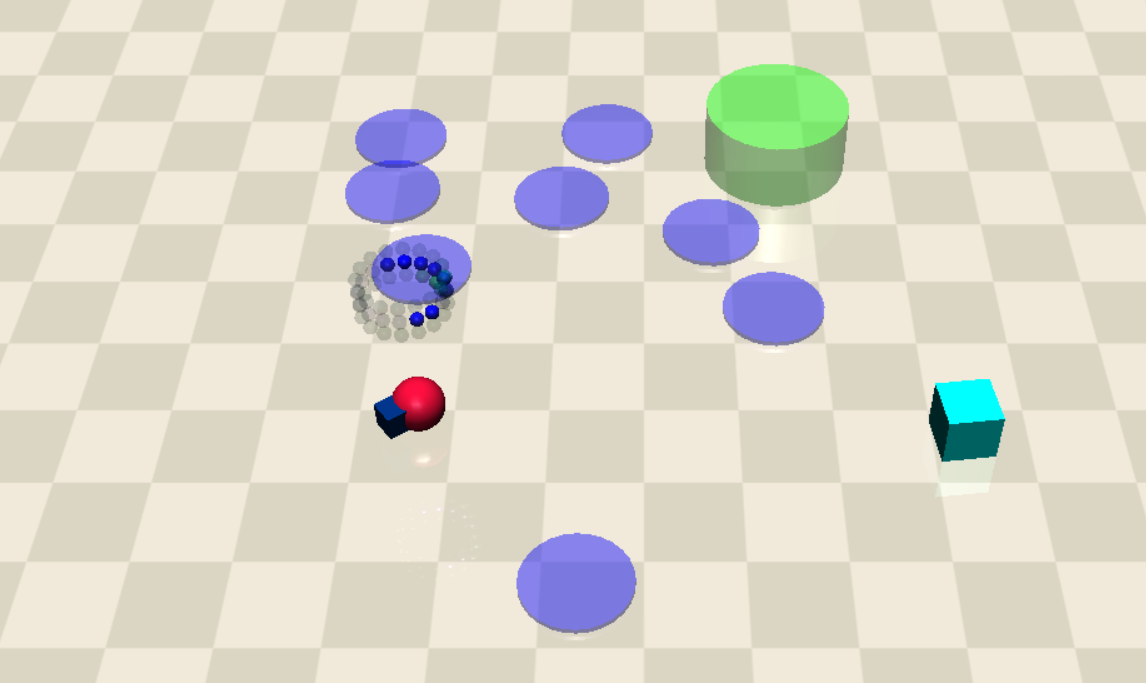
\includegraphics [width=0.4\textwidth, height=0.25\textwidth]{images/goal.png}}
    \subfloat[Circle Task]{
            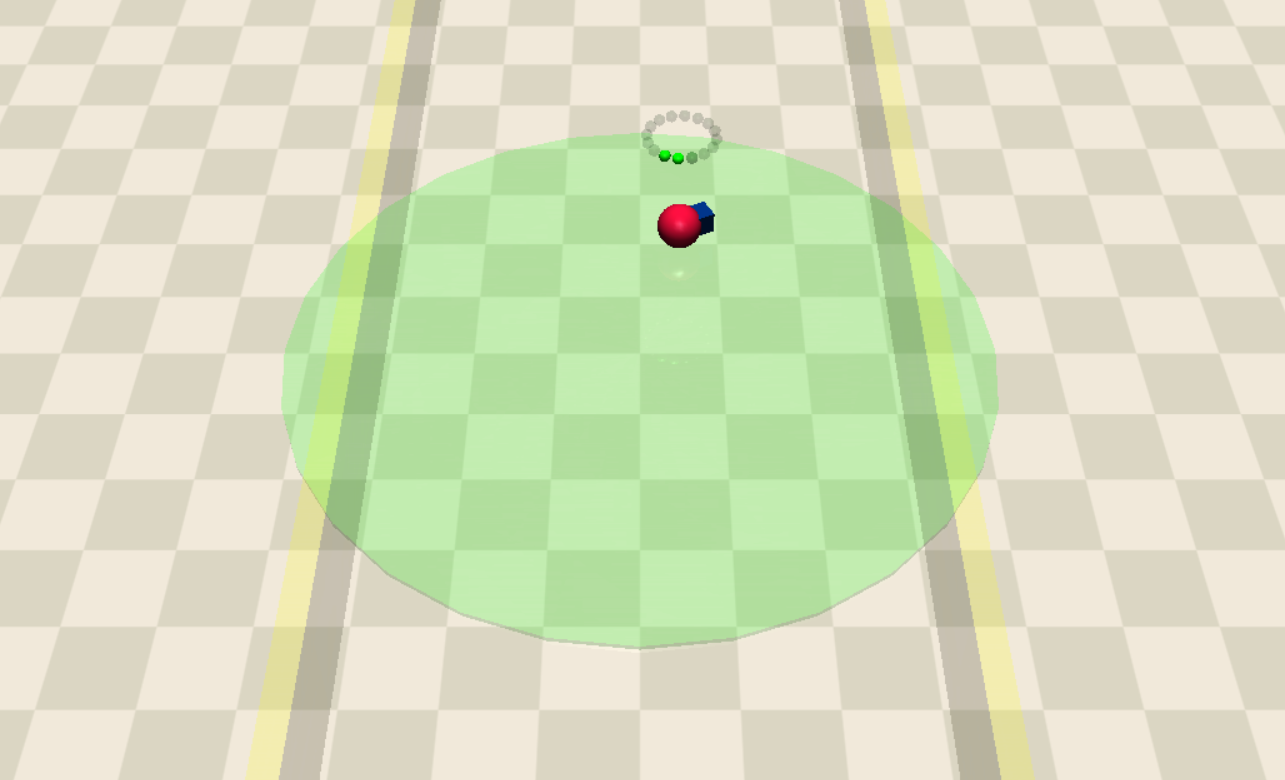
\includegraphics [width=0.4\textwidth, height=0.25\textwidth]{images/circle.png}}
    \\
    \subfloat[Push Task]{
            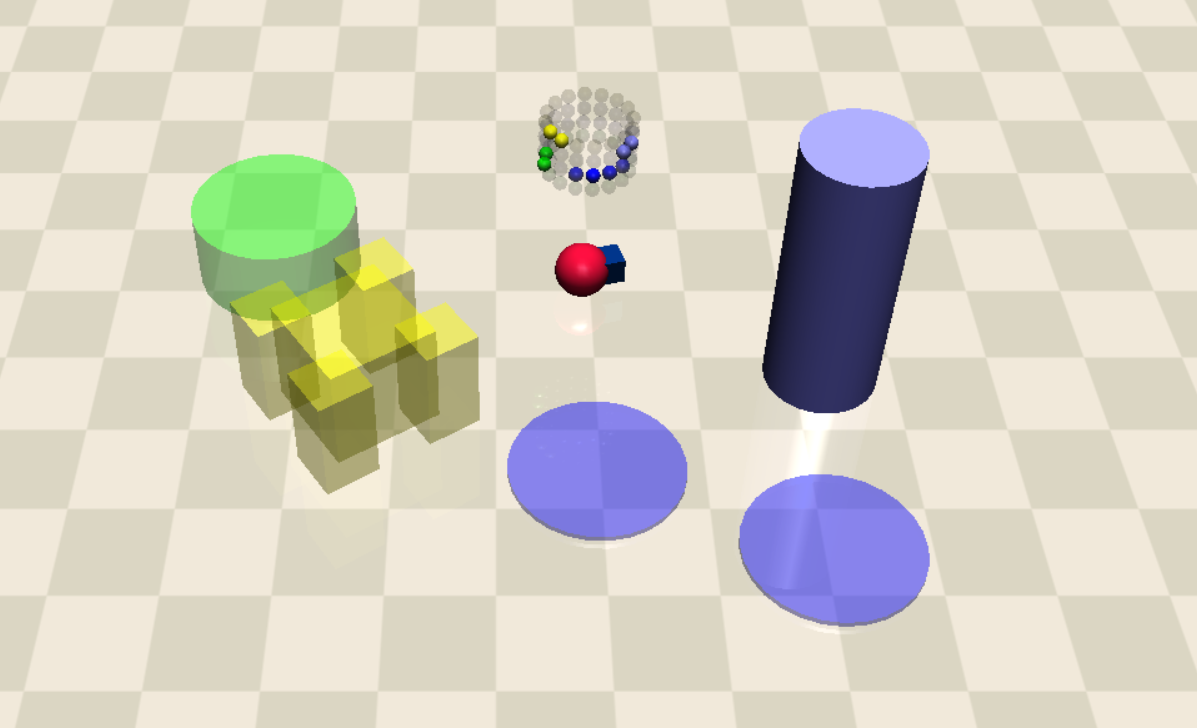
\includegraphics [width=0.4\textwidth, height=0.25\textwidth]{images/push.png}}
    \subfloat[MultiGoal Task]{
            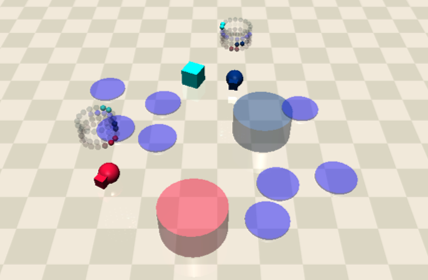
\includegraphics [width=0.4\textwidth, height=0.25\textwidth]{images/multiGoal.png}}
    \caption{不同任务场景图}
    \end{figure}

\subsection{安全可达空间实验}
为刻画机器人在不确定环境中的可行运动范围，本文基于包含智能体状态及环境观测的离线数据，对系统进行可达性分析预训练，从而构建机器人的安全可达空间。该安全空间用于刻画在给定动力学约束和环境条件下，系统状态是否能够在未来演化过程中满足安全约束，为后续在线决策提供安全判据。

通过对离线数据进行可达性分析，可以在状态空间中学习得到一类安全值函数，从而衡量不同状态的安全程度。如图 ~\ref{fig:safety_space} 所示，其中蓝色标记的区域表示安全值大于 0，说明系统在该区域内存在潜在的安全风险，即危险区域；其余区域则对应安全值小于等于 0，被视为满足安全约束的安全区域。该分布结果表明，可达性分析能够有效区分安全与非安全状态，为后续安全控制提供明确的边界信息。

此外，当改变机器人速度的大小与运动方向时，可以观察到安全域分布的显著变化。表明，安全可达空间与机器人的运动状态的相关性。当智能体速度增大或朝向发生变化时，其在有限时间内的可达集合随之改变，安全域边界也会发生调整。

上述结果表明，基于可达性分析构建的安全空间能够较好地反映环境风险与运动状态之间的关系。将该安全空间作为先验信息引入后续策略学习过程，有助于强化学习策略在在线决策时获得更明确的安全约束参考。
\begin{figure*}[thpb]
	\centering
	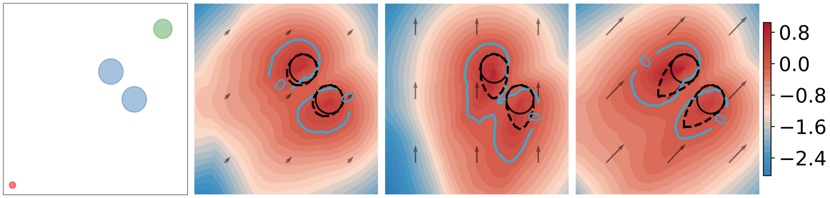
\includegraphics[width=\textwidth]{images/safe_space.png}
	\caption{安全空间分布图。蓝色曲线所包围的区域（安全值 > 0）表示危险区域，其余区域为安全区域。安全域会随着输入速度和方向的变化而发生改变。}
	\label{fig:safety_space}
\end{figure*}

\subsection{对比实验}
为评估完整框架在安全性与任务性能上的综合表现，本文在 Safety-Gymnasium 的 Goal、Circle、Push 与 MultiGoal 任务中与其他基准算法进行对比。

\subsubsection{基线方法}
本文在单智能体和多智能体场景中，与多种经典的安全强化学习算法进行对比，包括 PPO~\cite{schulman2017ppo}、 PCPO~\cite{yang2020projection} 、 PPO-Lag~\cite{stooke2020responsive} 、 TRPO-Lag~\cite{achiam2017cpo} ，多智能体实验包含了 MAPPO 、 HAPPO~\cite{kuba2022happo} 、 MACPO 以及 MAPPO\_Lag。

需要注意的是，ATACOM~\cite{liu2022atacom} 需要任务特定的约束雅可比矩阵以及扩展动作空间，因此在 Safety-Gymnasium 基准环境上进行直接比较较为困难；相比之下，本文的方法采用一种基于距离的简化安全过滤器，用于在点机器人任务中近似实现流形投影。

\subsubsection{评估指标与实现细节}

\begin{itemize}
\item \textbf{Reward}：每个回合的累计奖励（越高越好）。
\item \textbf{Cost}：累计约束违反次数（越低越好，理想值为 0）。
\item \textbf{Steps}：回合长度（直到到达目标或达到时间上限的步数）。
\end{itemize}

表~\ref{tab:hyperparams} 总结了实验中的关键超参数。所有实验均以 PPO~\cite{schulman2017ppo} 作为基础强化学习算法。表~\ref{tab:main_results} 和表~\ref{tab:ablation} 中的每个配置均在 3 个随机种子下训练 $10^5$ 个时间步；表~\ref{tab:ekf_comparison} 使用 5 个随机种子。基线方法报告平均性能，而 CMPL 报告 mean ± std。

\begin{table}[t]
\centering
\caption{实验超参数设置}
\label{tab:hyperparams}
\resizebox{0.8\columnwidth}{!}{
\begin{tabular}{ll|ll}
\toprule
\multicolumn{2}{c|}{\textbf{PPO 与训练参数}} & \multicolumn{2}{c}{\textbf{安全过滤器与 EKF}} \\
\midrule
学习率 & $3 \times 10^{-4}$ & 基础危险半径 $d_0$ & 0.6,m \\
折扣因子 $\gamma$ & 0.99 & 停止半径 $d_{\text{stop}}$ & 0.3,m \\
GAE 参数 $\lambda$ & 0.95 & 危险区域半径 $d_{\text{hazard}}$ & 0.2,m \\
网络结构 & MLP(256, 256) & 奖励校准权重 $\lambda$ & 0.1 \\
Rollout 缓冲区 & 2048 步 & 修正增益 $K_c$ & 10.0 \\
训练步数 & $10^5$ & EKF 窗口长度 $L$ & 10 \\
评估回合数 & 50 & CNN 架构 & Conv1d $\rightarrow$ FC \\
随机种子 (表 I,III / IV) & 3 / 5 & CNN 参数量 & $\sim$5K \\
Batch size (PPO) & 64 & 预训练轮数 & 100 \\
Clip ratio $\epsilon$ & 0.2 & 安全裕度参数 $\eta$ / $\delta$ & 0.1,m / 1.0 \\
&  & 噪声参数 $\sigma_{\text{base}}$ / $k$ & 0.1,m / 5.0 \\
\bottomrule
\end{tabular}
}
\end{table}

% 为系统性验证所提出约束流形方法在安全关键任务中的有效性，本文在 Safe-Policy-Optimization（SafePO）（Ji 等人，2023）实验平台上进行了广泛评估，并与多种代表性的安全强化学习方法进行了对比实验。SafePO 平台提供了标准化的安全强化学习基准任务与评估接口，能够较为全面地反映不同算法在安全性与性能之间的权衡能力。

% 本文选用累计奖励（Reward）和累计成本（Cost）作为主要评估指标，其中成本值越低表示策略越安全。考虑到机器人系统通常属于安全关键型应用场景，本文在实验评估中将安全性作为首要指标，在满足安全约束的前提下进一步追求更高的任务回报。为增强不同方法在安全维度上的区分度，并突出安全约束的重要性，本文对 SafePO 中的原始奖励函数进行了改造，引入了不同强度的碰撞惩罚项，并系统分析了碰撞惩罚强度变化对各类方法性能的影响。

\subsubsection{实验结果}
实验结果汇总于表~\ref{tab:main_results} 中。
本文的方法（CMPL）在所有任务和惩罚设置下都取得了最低的代价（cost），表明该方法对惩罚参数调节具有很强的鲁棒性。相比之下，基线方法对惩罚系数非常敏感。例如，在 Goal 任务中，PPO-Lag 的 cost 从 5.46（$r_{\text{col}}=0.1$）变化到 13.91（$r_{\text{col}}=0.5$），波动达到 $2.5\times$。
在 Circle 和 Push 任务中，基线方法仍表现出较明显的约束违背，cost 大致分布在 5-38 之间；相比之下，CMPL 的 cost 始终维持在较低水平，Circle 任务为 1.38-1.55，Push 任务为 0.92-1.23。可以看到，当碰撞惩罚降低至 $r_{\text{col}}=0.1$ 时，cost 有小幅上升。其原因在于，较低的碰撞惩罚会使强化学习策略更倾向于选择激进探索动作，这类动作虽然可能提高短期任务收益，但也会给安全过滤器带来更大的修正压力。

从回合长度来看，CMPL 在不同 $r_{\text{col}}$ 设置下变化较小，例如 Goal 任务基本保持在 350 步左右。这一现象与安全过滤机制有关：当机器人接近障碍物时，安全过滤器会对动作进行修正并限制其运动速度，而该过程并不依赖奖励函数中的碰撞惩罚系数。相较而言，部分基线方法在低惩罚设置下更容易选择距离障碍物较近的路径，甚至以更高风险换取更短的到达时间，因此回合长度会出现下降。需要注意的是，CMPL 在维持低约束违背的同时，并未明显牺牲任务收益，在 Goal 和 Push 任务中仍取得较高奖励，说明约束流形过滤机制能够在安全性和任务性能之间保持较好的协调。

在包含两个智能体的 Multi-Goal 任务中，约束违背主要来自智能体之间的相互碰撞以及智能体与障碍物之间的碰撞。由于多智能体场景中的交互关系更加复杂，所有基线方法的 cost 均处于较高水平，约为 $12.48$-$36.13$。CMPL 则将 cost 降至 $0.07$，同时仍保持正向奖励。该结果说明，本文提出的约束流形安全过滤方法并不局限于单智能体避障任务，也可以扩展到多智能体场景中，用于同时处理静态障碍物避让和智能体间避碰问题。
\begin{table*}[h!]
    \begin{center}
      \caption{Safety-Gymnasium 在不同任务和惩罚系数设置下的结果}
      \label{tab:main_results}
      \resizebox{\textwidth}{26mm}{
      \begin{tabular}{cc|*{4}{ccc|}ccc} \hline
      \multicolumn{2}{c|}{Algorithm} &
      \multicolumn{3}{c|}{PPO} &
      \multicolumn{3}{c|}{PCPO} &
      \multicolumn{3}{c|}{PPO\_Lag} &
      \multicolumn{3}{c|}{TRPO\_Lag} &
      \multicolumn{3}{c}{CMPL}\\
      TASK & $r_{collision}$
          & reward & cost & step
          & reward & cost & step
          & reward & cost & step
          & reward & cost & step
          & reward & cost & step \\ \hline

      \multirow{3}{*}{GOAL}
      & 1
          & -6.87 &  7.77 & 516
          & -2.11 &  3.75 & 342
          & -9.67 & 10.00 & 713
          & -3.08 &  4.01 & 490
          &  \textcolor{red}{1.68}{\tiny$\pm$0.3} &  \textcolor{Green3}{\textbf{0.00}} & 352{\tiny$\pm$18} \\
      & 0.5
          & -2.71 &  8.45 & 335
          & -0.71 &  4.66 & 252
          & -5.91 & 13.91 & 505
          &  0.00 &  3.53 & 226
          &  \textcolor{red}{1.72}{\tiny$\pm$0.4} &  \textcolor{Green3}{\textbf{0.00}} & 348{\tiny$\pm$21} \\
      & 0.1
          & 1.59 & 4.88 & 101
          & 1.65 & 3.94 & 101
          & 1.50 & 5.46 & 119
          & \textcolor{red}{1.79} & 3.01 & 84
          & 1.69{\tiny$\pm$0.3} & \textcolor{Green3}{\textbf{0.00}} & 352{\tiny$\pm$19} \\ \hline

      \multirow{3}{*}{CIRCLE}
      & 1
          & 5.88 & 5.49 & 500
          & 30.36 & 2.64 & 500
          & 8.14 & 6.82 & 500
          & \textcolor{red}{34.61} & 2.13 & 500
          & 16.42{\tiny$\pm$1.8} & \textcolor{Green3}{1.38}{\tiny$\pm$0.5} & 500 \\
      & 0.5
          & 23.24 & 8.51 & 500
          & 31.32 & 3.24 & 500
          & \textcolor{red}{33.67} & 5.00 & 500
          & 32.68 & 4.78 & 500
          & 17.05{\tiny$\pm$2.1} & \textcolor{Green3}{1.42}{\tiny$\pm$0.6} & 500 \\
      & 0.1
          & \textcolor{red}{38.32} & 31.83 & 500
          & 34.47 & 15.59 & 500
          & 37.14 & 23.98 & 500
          & 36.91 & 38.13 & 500
          & 18.23{\tiny$\pm$2.4} & \textcolor{Green3}{1.55}{\tiny$\pm$0.7} & 500 \\ \hline

      \multirow{3}{*}{PUSH}
      & 1
          & -10.43 & 9.99 & 996
          & -5.02 & 4.88 & 986
          & -8.71 & 8.52 & 992
          & -2.76 & 2.89 & 978
          &  \textcolor{red}{0.38}{\tiny$\pm$0.4} & \textcolor{Green3}{0.92}{\tiny$\pm$0.4} & 995{\tiny$\pm$3} \\
      & 0.5
          & -4.13 & 8.45 & 990
          & -3.30 & 6.50 & 989
          & -5.27 & 9.31 & 993
          & -2.99 & 6.49 & 967
          & \textcolor{red}{0.51}{\tiny$\pm$0.5} & \textcolor{Green3}{1.07}{\tiny$\pm$0.5} & 997{\tiny$\pm$2} \\
      & 0.1
          & -1.50 & 18.31 & 977
          & -0.74 & 11.93 & 947
          & -1.09 & 14.88 & 969
          & -1.10 & 13.28 & 978
          & \textcolor{red}{0.67}{\tiny$\pm$0.5} & \textcolor{Green3}{1.23}{\tiny$\pm$0.6} & 998{\tiny$\pm$2} \\ \hline

      \multicolumn{2}{c|}{Algorithm} &
      \multicolumn{3}{c|}{MAPPO} &
      \multicolumn{3}{c|}{HAPPO} &
      \multicolumn{3}{c|}{MACPO} &
      \multicolumn{3}{c|}{MAPPO\_Lag} &
      \multicolumn{3}{c}{CMPL}\\
      TASK & $r_{collision}$
          & reward & cost & step
          & reward & cost & step
          & reward & cost & step
          & reward & cost & step
          & reward & cost & step \\ \hline

      MULTI\_GOAL
      & 1
          & -23.42 & 23.12 & 362
          & -17.75 & 17.64 & 199
          & -36.41 & 36.13 & 182
          & -13.50 & 12.48 & 192
          & \textcolor{red}{0.01}{\tiny$\pm$0.2} & \textcolor{Green3}{0.07}{\tiny$\pm$0.1} & 346{\tiny$\pm$15}
  \\ \hline

      \end{tabular}
      }
    \end{center}
  \end{table*}
\subsection{消融实验}
在单智能体导航避障任务中，为更真实地刻画实际机器人在感知与定位过程中面临的不确定性，本文通过在环境中引入随机噪声来模拟传感器误差。
采用 PPO 算法作为基础强化学习方法，通过在 PPO 基线方法上逐步加入各个模块，
验证每个组件的贡献。实验结果为 3 个随机种子、$10^5$ 训练步以及 50 个评估回合的平均值。完整系统在速度相关传感器噪声条件下运行（$\sigma_{\text{base}} = 0.1$m，$k=5$）（见表~\ref{tab:ablation}）。
\begin{table}[t]
\centering
\caption{Goal 任务消融实验结果}
\label{tab:ablation}
\begin{tabular}{l|cc}
\toprule
配置 & Reward & Cost \\
\midrule
PPO（baseline） & $19.08 \pm 4.93$ & $64.59 \pm 8.51$ \\
+流形过滤器 & $12.20 \pm 5.06$ & $38.22 \pm 13.61$ \\
+可达性预训练 & $-8.44 \pm 8.21$ & $18.97 \pm 9.00$ \\
+EKF（完整系统，含噪声） & $-4.32 \pm 3.68$ & $\mathbf{12.51 \pm 6.32}$ \\
  \midrule
  完整系统（无奖励校准） & $16.83 \pm 0.92$ & $71.63 \pm 10.02$ \\
  \bottomrule
  \end{tabular}
  \end{table}

\begin{figure}[t]
\centering

\includegraphics[width=\linewidth]{images/training_curves.png}
\caption{学习曲线体现各组件的贡献。(a) 不同配置下的回合奖励；(b) 回合 cost（安全违规次数）}
\label{fig:training_curves}
\end{figure}

图~\ref{fig:training_curves} 展示了各配置的训练曲线。结果表明，每个组件都对整体性能产生了重要贡献：
\begin{itemize}
\item \textbf{流形过滤器（Manifold Filter）}：通过零空间投影（null-space projection）将 cost 降低了 41\%（$64.59 \rightarrow 38.22$），但由于不安全动作被修正，reward 有一定下降。

\item \textbf{可达性预训练（Reachability Pretraining）}：通过将策略约束在可行区域 $\mathcal{S}^*_f$ 内，并引入更大的安全裕度，使 cost 相比基线进一步降低了 71\%（$64.59 \rightarrow 18.97$）。

\item \textbf{数据驱动 EKF}：即使在速度相关的传感器噪声存在的情况下，仍然能够保持相近的安全性（$12.51$），说明该方法在感知不确定性下依然能够稳健地执行约束。

\item \textbf{奖励校准（Reward Calibration）}：对安全性至关重要——如果移除该机制，智能体会利用约束边界来获得更高奖励（$16.83$），但同时会产生显著更多的违规（$71.63$ 对比 $12.51$）。
\end{itemize}

\subsection{EKF 对比实验}
为了单独评估 EKF 的贡献，首先在无噪声条件下训练一个带安全过滤器的单智能体策略，然后在部署阶段引入速度相关噪声~\eqref{eq:vel_noise}（$\sigma_{\text{base}} = 0.1$m，$k = 5$），并比较三种状态估计配置。表~\ref{tab:ekf_comparison} 给出了在 5 个随机种子和 50 个评估回合上的平均结果。

\begin{table}[t]
\centering
\caption{Goal 任务 EKF 对比实验}
\label{tab:ekf_comparison}
\resizebox{0.8\columnwidth}{!}{
\begin{tabular}{l|ccc}
\toprule
方法 & 位置误差 (m) & Reward & Cost \\
\midrule
原始 GPS & $0.54 {\pm} 0.18$ & $-7.92 {\pm} 1.43$ & $9.14 {\pm} 2.37$ \\
EKF（固定 $R$） & $0.41 {\pm} 0.13$ & $-7.86 {\pm} 1.21$ & $9.58 {\pm} 2.15$ \\
EKF（学习得到的 $R$） & $\mathbf{0.27 {\pm} 0.05}$ & $-7.87 {\pm} 0.94$ & $\mathbf{9.31 {\pm} 1.68}$ \\
\bottomrule
\end{tabular}
}
\end{table}

采用学习得到协方差矩阵的 EKF 在位置精度方面表现最佳（$0.27$m），相比原始 GPS 将误差降低了 49\%，相比固定 $R$ 的 EKF 降低了 34\%。同时，其误差方差也显著降低，为原始 GPS 的约 $1/3.6$（$0.05$ 对比 $0.18$）。

虽然在这一独立评估中各方法的 cost 差异不大，但消融实验（表~\ref{tab:ablation}）展示了完整系统的优势：在包含传感器噪声的训练条件下，cost 从 $18.97$ 进一步降低到 $12.51$。

\textbf{计算开销。} NoiseAdapter CNN 带来的计算开销非常小：该网络约有 5K 个参数，在 CPU 上每一步推理时间小于 $0.1$,ms，相比环境步进时间（5ms）和 PPO 前向传播时间（1ms）几乎可以忽略不计。

预训练阶段需要进行 30 次随机探索回合（约 2 分钟）以及 100 个 epoch 的负对数似然（NLL）优化（约 30 秒），这是一次性的开销，可以在整个训练过程中被摊销。

实验表明，该 CNN 在约 50 个 epoch 内即可收敛（损失在约 $-3.7$ 处进入平台期）。学习得到的 $R_t$ 能够实现平滑自适应：在高速运动时预测较大的测量噪声协方差，在低速运动时预测较小的协方差，这与理论上的速度—噪声模型~\eqref{eq:vel_noise} 相一致。

\subsection{Webots 仿真实验}
本文在 Webots~\cite{webots2004} 仿真环境中的 E-puck 机器人上验证了安全过滤器和 EKF 的有效性。为了测试方法对控制策略的策略无关迁移能力（policy-agnostic transferability），实验中刻意使用 P 控制器（而非强化学习策略）进行控制。

通过 ROS 2 验证了系统部署，使用 webots\_ros2\_driver 进行仿真接口集成，其中安全过滤器作为独立的 ROS2 节点运行（见图~\ref{fig:ros2arch}）。
\begin{figure}[t]
\centering

\includegraphics[width=\columnwidth]{images/ros_architecture.png}
\caption{ROS2 集成架构}
\label{fig:ros2arch}
\end{figure}

为了验证安全层具有策略无关性（policy-agnostic），本文在 E-puck 机器人（直径 $\varnothing70mm$）上部署了基于距离的安全过滤器和标准 EKF（固定 $R$），并在 Webots 仿真环境中进行实验。实验场景为一个 $2\text{m} \times 2\text{m}$ 的区域，其中放置 6 个圆柱形障碍物，GPS 噪声为 $\sigma=0.04$m，IMU 航向角噪声为 $\sigma=0.05$,rad。名义控制策略刻意采用一个简单的 P 控制器——而不是训练得到的强化学习策略——以证明该安全架构可以在无需重新训练的情况下迁移到新的机器人平台和控制器上。

在 Webots 实验中，安全过滤器采用基于距离的速度缩放机制（相比流形过滤器更为简单），同时使用具有固定噪声协方差的标准 EKF。实验结果如图~\ref{fig:ros}，在没有安全过滤的情况下，20 次实验中有 8 次发生碰撞（碰撞率 40\%），其中 4 次由于碰撞导致导航错误而未能到达目标（成功率 80\%）。而本文的方法实现了零碰撞，成功率达到 85\%。其中 3 次失败是由于机器人在密集障碍区域附近发生导航超时，但均在没有碰撞的情况下安全结束。值得注意的是，安全过滤器实际上提高了成功率（85\% 对比 80\%），因为未过滤的碰撞会破坏导航稳定性。EKF 通过融合里程计和 GPS 测量，将位置误差降低了 27\%（$0.051 \rightarrow 0.037$m）（见表~\ref{tab:webots}）。

\begin{table}[t]
\centering
\caption{Webots E-puck 实验验证}
\label{tab:webots}
\begin{tabular}{l|cc}
\toprule
指标 & 无过滤 & \textbf{本文方法（完整系统）} \\
\midrule
成功率 (\%) & 80.0 & $\mathbf{85.0}$ \\
碰撞率 (\%) & 40.0 & $\mathbf{0.0}$ \\
位置误差 (m) & $0.051 \pm 0.001$ & $\mathbf{0.037 \pm 0.001}$ \\
路径长度 (m) & $\mathbf{0.94 \pm 0.41}$ & $1.80 \pm 1.49$ \\
\bottomrule
\end{tabular}
\end{table}

\begin{figure*}[t]
\centering
\subfloat[实验环境]{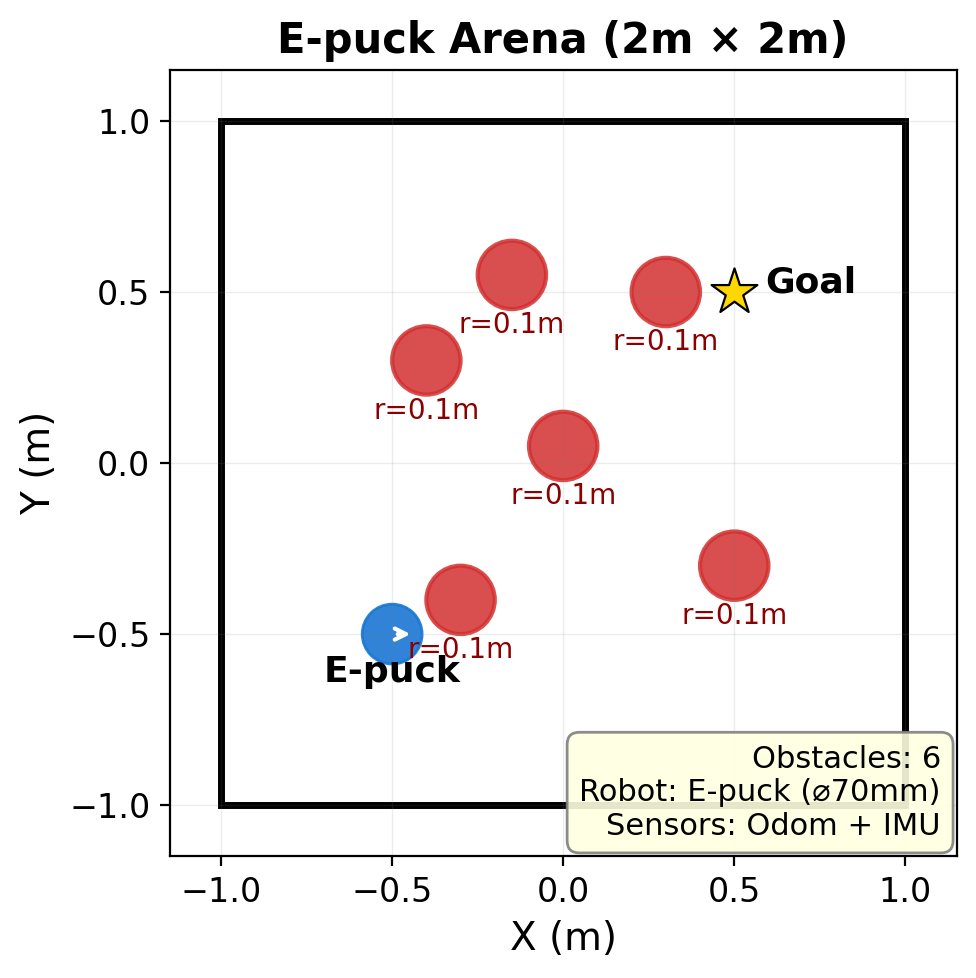
\includegraphics[height=4cm]{images/ros_setup.png}}
\hfill
\subfloat[轨迹对比]{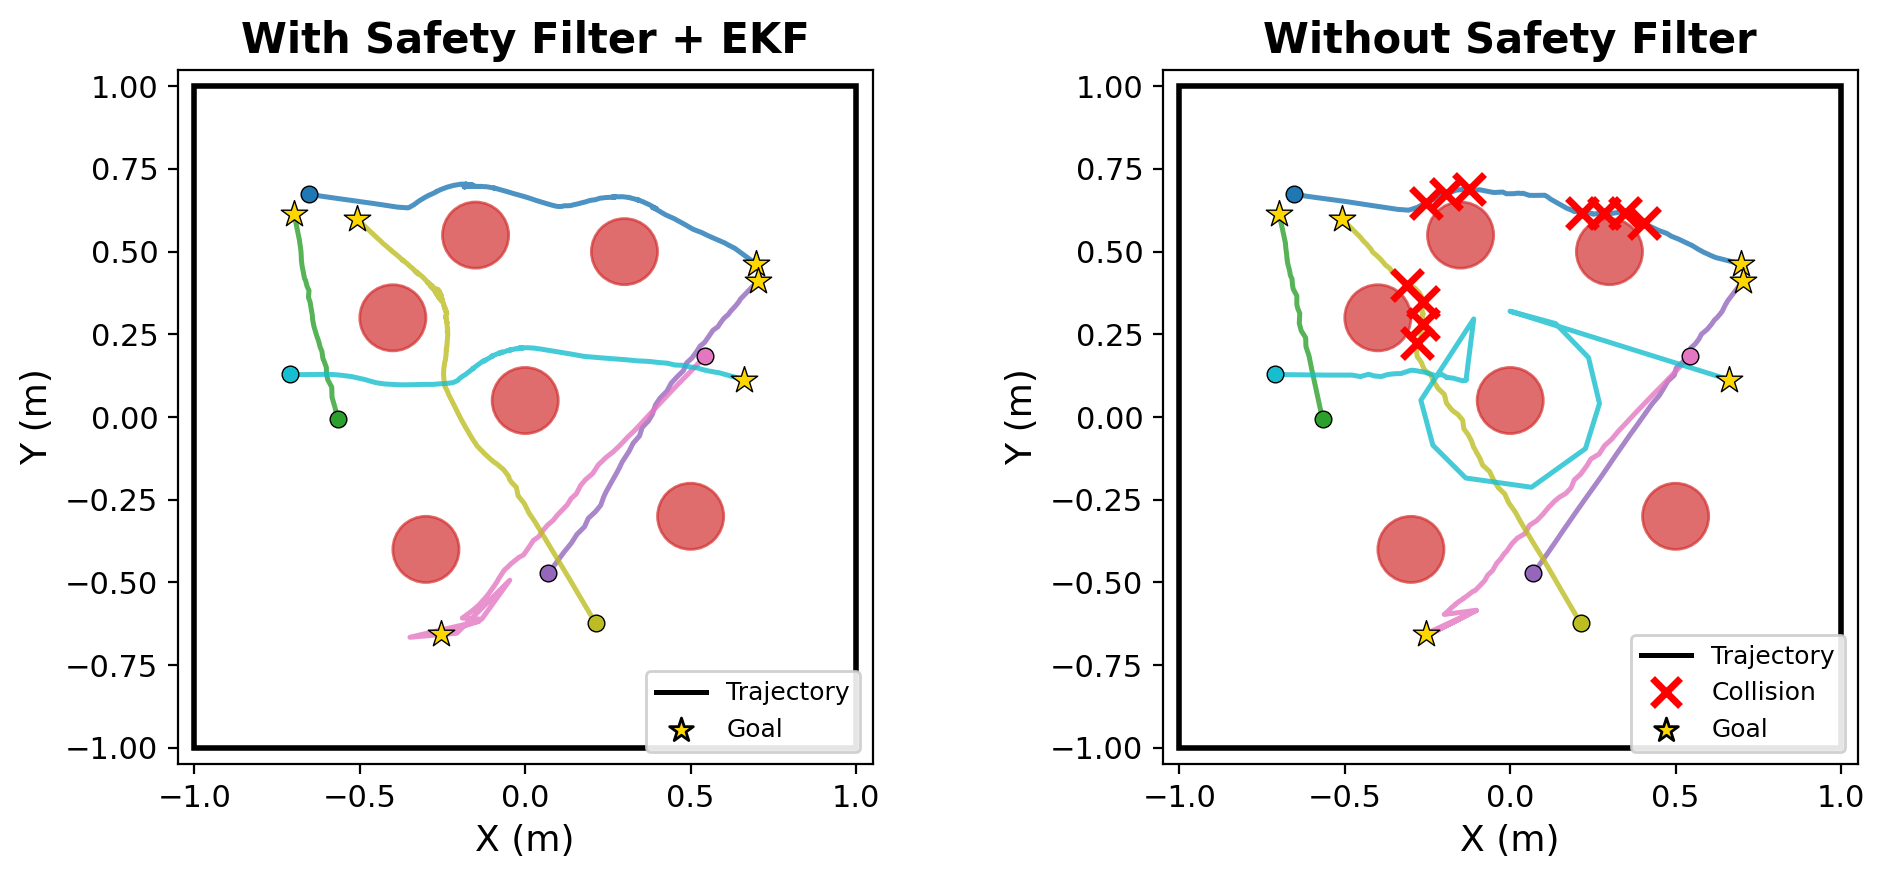
\includegraphics[height=4cm]{images/trajectory.png}}
\caption{Webots 中 E-puck 实验验证。(a) 含 6 个障碍物的实验环境。(b) 轨迹对比：带安全过滤器 + EKF（左）与无过滤（右，$\times$ 表示碰撞）。}
\label{fig:ros}
\end{figure*}



% \subsection{ROS平台验证实验}

% 为进一步验证所提出安全强化学习框架在实际机器人系统中的可行性与工程适用性，本文将该方法部署至 ROS 平台，并在 Webots 仿真环境中开展导航避障实验。实验对象选用 E-puck 移动机器人模型，通过其搭载的 IMU 传感器获取运动状态信息，并结合所提出的数据驱动定位算法，实现对机器人位姿的在线估计与更新。
% \begin{figure}
%     \centering
%     
\includegraphics[width=1\linewidth]{images/ros_architecture.png}
%     \caption{ros architecture}
%     \label{fig:placeholder}
% \end{figure}
% 在实验过程中，机器人在包含静态障碍物的环境中执行自主导航任务，目标是在满足安全约束的前提下，从初始位置安全到达指定目标点。系统通过 ROS 框架完成传感器数据的采集、状态估计、策略推理以及控制指令的发布，同时利用 rviz 可视化工具对机器人运动轨迹进行实时显示与分析。实验结果如图 4(b) 所示，其中蓝色轨迹表示 Webots 仿真环境中机器人的真实运动轨迹，红色轨迹表示由所提出的数据驱动定位算法估计得到的轨迹。

% 从实验结果可以看出，红色估计轨迹与真实轨迹整体保持较高的一致性，表明所提出的定位方法能够在存在传感器噪声的情况下较为准确地估计机器人位姿。同时，在策略执行过程中，机器人能够有效避开环境中的障碍物，并在未发生安全约束违规的情况下顺利到达目标位置，验证了所提出安全策略在实际控制回路中的有效性与稳定性。

% 上述 ROS 平台与 Webots 仿真环境下的实验结果表明，本文提出的安全强化学习框架不仅在理论和仿真层面具有良好性能，同时具备较强的工程实现能力，为未来向真实机器人系统的迁移与应用奠定了坚实基础。

% \begin{figure}[thpb]
% \centering
% %\includegraphics[width=3in]{fig5}
% \subfloat[Experimental Scenario]{
% 		
\includegraphics [width=0.4\textwidth, height=0.4\textwidth]{任务1-MICL-2023-ConstrainedMARL-ConstrainedfactorSLAM/IROS/ROS.png}}
% \subfloat[Robot Trajectory]{
% 		
\includegraphics [width=0.4\textwidth, height=0.4\textwidth]{任务1-MICL-2023-ConstrainedMARL-ConstrainedfactorSLAM/IROS/轨迹.jpg}}
% \caption{ROS Platform Verification Experiment}
% \end{figure}

\section{本章小结}

本章围绕安全强化学习在机器人导航避障问题，构建了安全可达空间刻画 + 策略生成 + 安全过滤 + 状态估计的CMPL框架。
针对强化学习策略在复杂场景下可能出现的约束违规风险，本文首先根据系统约束构建安全可达空间，为在线决策提供风险边界，
并进一步从约束流形视角设计了安全过滤机制，
通过对名义动作进行在线修正，在不改变上层策略结构的前提下实现对安全约束的显式满足，并给出了相应的稳定性分析。

同时，为提升系统在噪声感知条件下的可用性，本章结合运动学模型与多源传感信息，构建了 EKF 状态估计模块，
并进一步引入基于数据驱动的观测噪声自适应建模，以增强定位精度与鲁棒性。
仿真实验结果表明，CMPL 在不同任务和控制策略下均能降低碰撞风险，并保持较好的任务表现。
上述工作为后续多机器人编队场景中的安全协同控制研究提供了方法基础。

\chapter{基于几何约束的策略学习方法}
第三章围绕智能体强化学习在复杂环境中的安全性问题，构建了基于约束流行的安全过滤机制，在一定程度上缓解了机器人在运动过程中的风险行为。然而，在多机器人协同任务中，系统不仅需要满足个体层面的安全可行性，还需在群体层面同时维持编队拓扑、相对位姿关系与任务协同效率，这使得控制目标由单一安全约束扩展为多任务耦合下的结构化优化问题。

基于此，第四章在第三章安全约束思想的基础上进一步强化与拓展，将安全约束从个体避碰推广至多机器人几何关系保持，使强化学习策略能够在满足安全边界的前提下，更有效地利用编队结构先验实现协同决策。由此，本章旨在继承第三章安全保证能力的同时，提升多机器人系统在复杂任务中的组织性、稳定性与控制性能。
\section{方法框架}
本文提出一种基于几何约束的策略学习方法（Geo-Constrained Policy Learning, GCPL），
通过融合强化学习与几何结构约束，实现多机器人系统在复杂环境中的安全协同与编队控制，系统整体控制流程可划分为候选动作生成、安全修正、解析合成、环境交互以及策略更新五个阶段。
\begin{figure}
    \centering
    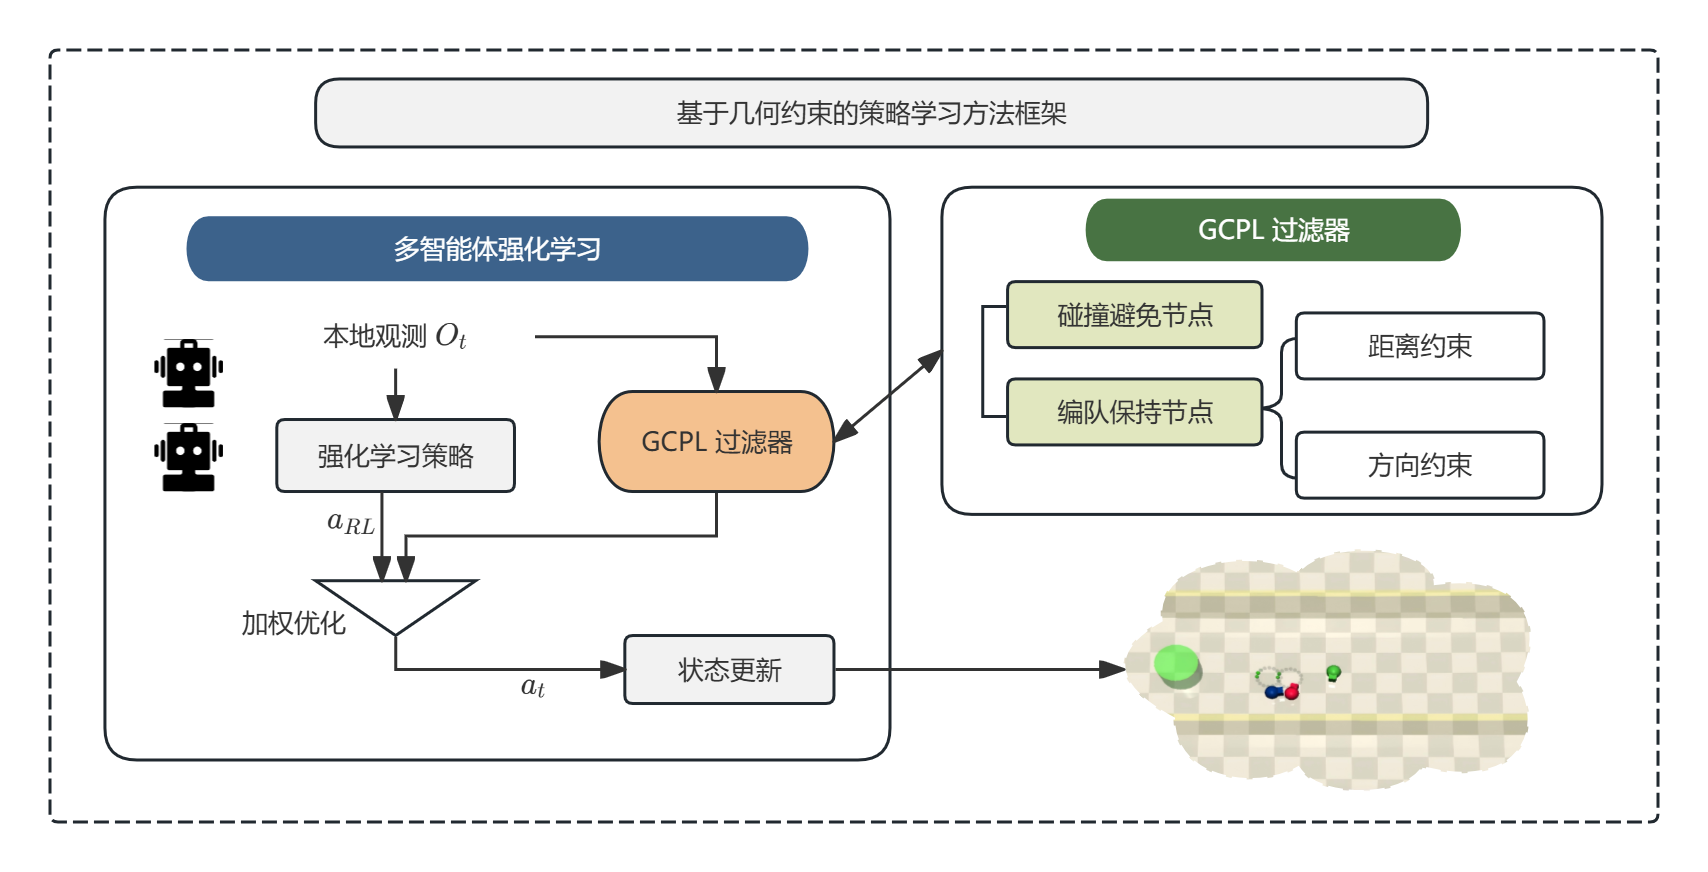
\includegraphics[width=1\linewidth]{images/RMPflow framework.png}
    \caption{GCPL 算法框架}
    \label{fig:RMPflow framework}
\end{figure}
在强化学习层，本文采用基于策略梯度的近端策略优化方法构建多智能体策略网络（Multi-Agent Proximal Policy Optimization，MAPPO）。策略网络以系统在时刻 $x_t$ 的观测状态作为输入，输出一个候选控制动作 $a^{RL}$。该候选动作主要反映任务层面的优化需求，包括尽可能缩短到达目标的时间、提升通过复杂区域时的效率以及维持更合理的编队形态等，但在这一阶段并未对机器人之间的安全距离或障碍物约束进行严格保证，因此其结果更多体现为策略在当前状态下给出的原始控制意图。

在几何过滤层，引入基于黎曼流形运动策略表示的控制框架，对强化学习产生的候选动作进行约束与融合。在该框架中，系统被组织为一棵任务树，树中每一个叶节点都对应一个具有明确几何含义的子任务，例如目标跟踪、障碍物规避、速度范围限制以及机器人之间的安全间距维持等。每个任务都以自然形式 $(f_i, M_i)$ 表示，其中 $f_i$ 描述任务空间中的期望控制动作，$M_i$ 则作为度量矩阵，用来刻画该任务在局部几何结构中的重要程度以及不同方向上的权重分布。强化学习输出的候选动作 $a^{RL}$ 在这一结构中被建模为一个额外的叶节点任务，并与其他安全相关任务共同参与后续的合成过程，使其影响受到整体几何约束的调节，而不是直接作用于系统。

在GCPL的计算过程中，各叶节点首先通过推前映射在各自的任务空间中完成评估，随后在拉回阶段通过雅可比映射被统一投影回根节点所在的空间。所有叶节点的自然形式在同一坐标框架下进行叠加，得到整体的广义力与度量矩阵：
\begin{equation}
(f_{total}, M_{total}) = \sum_i Pullback(f_i, M_i).
\end{equation}
这一过程本质上是在统一的几何度量下对多个任务进行一致性整合，使得不同任务在系统状态变化时能够通过各自的度量矩阵自动调整权重。当某一约束在当前情形下更为关键时，其对应的度量值会明显增大，从而在合成结果中产生更强的影响，而其他任务的作用则相对减弱，这样可以在不引入硬切换的情况下缓解任务之间的冲突。

当所有任务信息汇总至根节点之后，系统通过解析步骤计算最终的控制输出：
\begin{equation}
a = M_{\text{total}}^{\dagger} f_{total},
\end{equation}
其中 $M_{\text{total}}^{\dagger}$ 表示度量矩阵的广义逆。该求解过程可以理解为在整体度量约束下，对各个任务期望进行加权后的最小二乘意义最优解。由此得到的加速度指令既包含了强化学习层所提供的任务驱动趋势，又在数值上受到安全相关任务的修正与限制，使其在满足几何一致性的同时保持物理上可实现。

机器人按照该安全修正后的控制量与环境进行交互，并转移到下一时刻的状态。环境根据编队保持情况、到达目标的效率以及是否违反安全约束等因素生成奖励信号 $r_t$，这一信号被反馈给 MAPPO 策略网络，用于更新策略参数。随着训练的不断推进，策略逐渐学会在其可行动作范围内输出更符合安全几何结构的控制意图，使得 GCPL 在在线修正时所需的调整幅度逐步减小，从而提升整体控制过程的平滑性与执行效率。
\begin{figure}
    \centering
    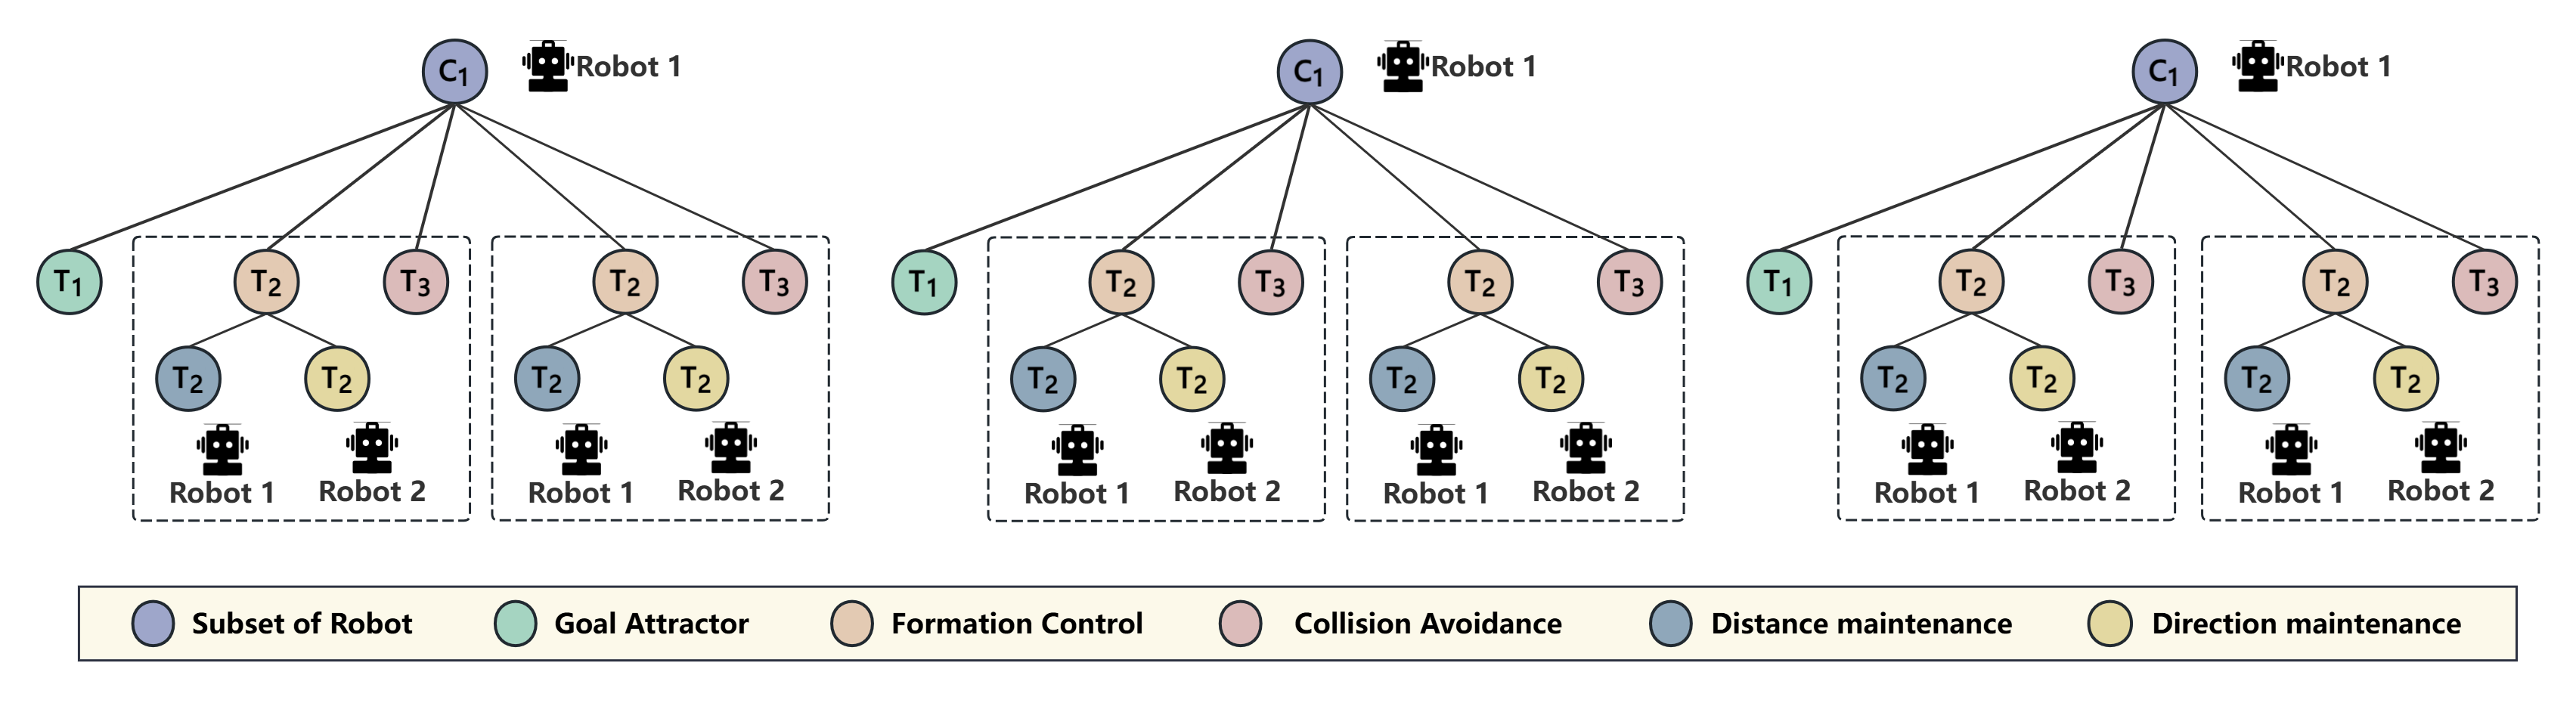
\includegraphics[width=1\linewidth]{images/rmpflow (1).png}
    \caption{GCPL任务树}
    \label{fig:RL-RMPflow树}
\end{figure}

\begin{algorithm}[t]
\caption{ GCPL 多机器人控制}
\label{alg:rl_rmpflow_simple}
\begin{algorithmic}[1]
\REQUIRE 多机器人初始状态 $x_0$，目标 $x_{\text{goal}}$，MAPPO 策略 $\pi_\theta$，几何任务集合 $\mathcal{T}$
\FOR{每个训练回合}
    \STATE 初始化环境与机器人状态 $x \leftarrow x_0$
    \FOR{每个时间步 $t$}
        \STATE \textbf{强化学习层：}每个机器人采样动作 $a^{RL}_{i,t} \sim \pi_\theta(o_{i,t})$
        \STATE \textbf{几何过滤层：}构建 RL 叶子节点和避障、编队任务节点
        \STATE 执行 pullback 及 合并：
        \[
        M_i = \sum_k M_{i,k}, \quad f_i = \sum_k f_{i,k}, \quad \ddot{x}_i = M_i^{-1} f_i
        \]
        \STATE 应用控制 $a_i$ 推进环境，计算奖励 $r_t$ 和代价 $c_t$
        \STATE 存储轨迹 $(o_t, a_t, r_t, c_t)$
    \ENDFOR
    \STATE 通过 MAPPO 更新策略参数 $\theta$
\ENDFOR
\end{algorithmic}
\end{algorithm}

\section{系统建模}
\subsection{状态与控制输入建模}
本文研究对象为工作在二维平面环境下的多差速移动机器人系统。为便于在 GCPL 框架下进行统一的几何力学建模与控制，首先对单个机器人进行状态与控制输入建模。
设机器人系统由若干个同构差速机器人组成，第 i 个机器人在平面内的配置空间状态可表示为机器人在世界坐标系下的平面位置坐标，以及当前航向角：
\begin{equation}
    q_i = (x_i,y_i,\theta_i)
\end{equation}

机器人的底层控制输入为前进线速度与转向角速度：
\begin{equation}
    u_i=(v_i,ω_i)
\end{equation}

GCPL 是在配置空间加速度层进行多任务融合的几何控制框架，本文将机器人控制问题建模为加速度级指令生成问题，即：
\begin{equation}
    \ddot{q_i} = a_i
\end{equation}
其中 $a_i =(a_x ,a_y)$为机器人质心在世界坐标系下的二维期望加速度。通过后续的运动学映射，可将该加速度指令转换为差速机器人可执行的线加速度与角加速度。
\subsection{编队的图建模}

为刻画多机器人系统的空间编队结构，本文采用无向图对编队拓扑进行建模。设系统包含 $N$ 个机器人，其在二维平面中的位置表示为
\begin{equation}
    p = (p_0, p_1, \ldots, p_{N-1}), \quad p_i \in \mathbb{R}^2.
\end{equation}

定义编队拓扑图为
\begin{equation}
    \mathcal{G} = (\mathcal{V}, \mathcal{E})
\end{equation}
其中节点集合 $\mathcal{V} = \{0,1,\ldots,N-1\}$ 表示机器人个体，边集合 $\mathcal{E} \subseteq \mathcal{V} \times \mathcal{V}$ 表示需要维持相对几何约束的机器人对。对于每一条边 $(i,j) \in \mathcal{E}$，指定期望的相对距离 $d_{ij}^* > 0$。

基于该图结构，定义编队的距离约束为
\begin{equation}
    \|p_i - p_j\| = d_{ij}^*, \quad \forall (i,j) \in \mathcal{E}.
\end{equation}

为刻画编队偏离程度，引入边的距离误差函数
\begin{equation}
    z_{ij} = \psi(p_i, p_j) = \|p_i - p_j\| - d_{ij}^*.
\end{equation}

进一步地，定义整体编队误差能量函数为
\begin{equation}
    E(p) = \frac{1}{2} \sum_{(i,j)\in\mathcal{E}} 
    \left( \|p_i - p_j\| - d_{ij}^* \right)^2,
\end{equation}
该能量函数用于度量当前编队与目标编队之间的整体偏差。

仅依赖距离约束时，编队结构在欧氏变换（平移与旋转）下是不变的，即该约束仅能保证编队的刚性形状，而无法唯一确定其方向与朝向。因此，为消除由旋转和镜像引起的不确定性，本文进一步在图结构上引入方向约束。

对于每一条边 $(i,j) \in \mathcal{E}$，定义单位方向向量为
\begin{equation}
    \hat{r}_{ij} = \frac{p_j - p_i}{\|p_j - p_i\|},
\end{equation}
并设定对应的期望方向 $\hat{r}_{ij}^*$。由此定义方向误差为
\begin{equation}
    z_{ij}^{\theta} = 1 - \hat{r}_{ij}^\top \hat{r}_{ij}^*.
\end{equation}

结合距离与方向约束，可得到联合编队能量函数
\begin{equation}
    E_{\text{form}}(p) = 
    \frac{1}{2} \sum_{(i,j)\in\mathcal{E}} 
    \left[
    \alpha_d \left( \|p_i - p_j\| - d_{ij}^* \right)^2
    +
    \alpha_\theta \left( 1 - \hat{r}_{ij}^\top \hat{r}_{ij}^* \right)^2
    \right],
\end{equation}
其中 $\alpha_d, \alpha_\theta > 0$ 分别为距离约束与方向约束的权重系数。

该图建模方法为后续编队保持节点的构建提供了统一的几何表示，同时也为强化学习奖励函数的设计提供了理论基础。

\subsubsection{不同编队形状的图结构构造}

在上述统一图建模框架下，不同编队形状可通过设计不同的边集合 $\mathcal{E}$ 及对应的期望距离 $d_{ij}^*$ 来实现。下面给出三种典型编队（直线、楔形和圆形）的图结构构造方法。

\paragraph{1) 直线编队（Line Formation）}

直线编队的目标是使机器人沿某一主轴方向排列，并仅维持相邻机器人之间的局部距离约束。设机器人按照索引顺序排列，则边集合定义为
\begin{equation}
    \mathcal{E}_{\text{line}} = \{ (i, i+1) \mid i = 0, 1, \ldots, N-2 \}.
\end{equation}

对应的期望距离通常设置为常数间距：
\begin{equation}
    d_{i,i+1}^* = d, \quad \forall (i,i+1) \in \mathcal{E}_{\text{line}}.
\end{equation}

该结构形成一条链式拓扑，仅约束局部相邻关系。由于该图不具备全局刚性，其整体朝向与宽度需要通过额外的方向约束或辅助奖励加以限制。

\paragraph{2) 楔形编队（Wedge Formation）}

楔形编队通常表现为以某一机器人为顶点的“V”字结构。设机器人 $0$ 为顶点，其余机器人分布在两侧，则边集合可构造为
\begin{equation}
    \mathcal{E}_{\text{wedge}} =
    \{ (0,i) \mid i = 1,\ldots,N-1 \}
    \cup
    \{ (i,j) \mid i,j \in \mathcal{N}_{\text{side}} \},
\end{equation}
其中 $\mathcal{N}_{\text{side}}$ 表示同侧机器人集合。

在实际实现中，可进一步为左右两侧分别定义不同的期望距离，以形成稳定的楔形夹角。例如，对于同一侧的相邻机器人：
\begin{equation}
    d_{ij}^* = d_{\text{side}}, 
\end{equation}
而对于顶点与侧边机器人：
\begin{equation}
    d_{0i}^* = d_{\text{apex}}.
\end{equation}

该结构通常构成刚性图，能够在二维平面中唯一确定编队形状（除整体刚体变换外）。

\paragraph{3) 圆形编队（Circle Formation）}

圆形编队的目标是使机器人均匀分布在一个圆周上。为此，可采用环形拓扑结构，即每个机器人仅与其相邻两个机器人建立连接：
\begin{equation}
    \mathcal{E}_{\text{circle}} =
    \{ (i, (i+1) \bmod N) \mid i = 0,1,\ldots,N-1 \}.
\end{equation}

对应的期望距离设置为相邻机器人在圆周上的弧长近似：
\begin{equation}
    d_{i,i+1}^* = 2R \sin\left(\frac{\pi}{N}\right),
\end{equation}
其中 $R$ 为期望圆半径。

\section{强化学习层}
强化学习层用于为多机器人系统提供目标导向的高层决策与性能优化能力，其核心目标是在满足安全与编队约束的前提下，提高机器人群体在复杂环境中的通行效率、路径平滑度与整体鲁棒性。由于系统中包含多个具有相互耦合动力学与协同约束的机器人个体，本文采用多智能体近端策略优化算法（Multi-Agent Proximal Policy Optimization, MAPPO）进行策略学习。

在每个决策时刻 $t$，系统状态表示为：
\begin{equation}
    s_t = \{x_1, \dot{x}_1, \ldots, x_N, \dot{x}_N, x_{\text{goal}}, \mathcal{O}\}
\end{equation}
其中 $x_i$ 与 $\dot{x}_i$ 分别表示第 $i$ 个机器人的位置与速度，$x_{\text{goal}}$ 为目标位置，$\mathcal{O}$ 表示环境障碍物信息。

策略网络为每个机器人输出其局部控制动作：
\begin{equation}
    a_{i,t}^{RL} \sim \pi_{\theta}(o_{i,t}), \quad i=1,\ldots,N
\end{equation}
其中 $o_{i,t}$ 为机器人 $i$ 在时刻 $t$ 的局部观测，$\pi_{\theta}$ 为共享参数的策略网络。最终动作向量可表示为：
\begin{equation}
    a_t^{RL} =
    \begin{bmatrix}
    a_{1,t}^{RL} \\
    \vdots \\
    a_{N,t}^{RL}
    \end{bmatrix},
    \quad
    a_{i,t}^{RL} \in \mathbb{R}^2
\end{equation}

该动作表示每个机器人在世界坐标系下的期望平面加速度，用于引导机器人向目标区域移动。通过共享策略参数，MAPPO 能够在保证个体决策独立性的同时学习到群体层面的协同行为。

\subsection{强化学习与几何控制的协同机制}
\subsubsection{几何叶节点设计}
为了使多智能体强化学习输出能够融入几何过滤层的控制框架，本文将每个机器人的策略输出构造为独立的 RL 叶子任务节点。对于机器人 $i$，其强化学习任务空间定义为：
\begin{equation}
    z_{RL,i} = \psi_{RL}(x_i) = x_i
\end{equation}

由于任务空间与配置空间一致，其 Jacobian 为：
\begin{equation}
    J_{RL,i} = I_2
\end{equation}

为调节强化学习任务在多任务融合中的影响力，定义度量矩阵为：
\begin{equation}
    M_{RL,i} = w_{RL} I_2
\end{equation}
其中 $w_{RL} > 0$ 为强化学习任务权重。

在自然形式下，RL 叶子节点的广义力为：
\begin{equation}
    f_{RL,i} = M_{RL,i} a_{i,t}^{RL}
\end{equation}

因此，每个机器人均对应一个强化学习节点：
\begin{equation}
    (f_{RL,i}, M_{RL,i})
\end{equation}
这些节点与避障、机器人间安全距离及编队保持等几何任务节点共同组成GCPL任务树，并在反向传播阶段进行度量加权融合。

在所提出的分层控制架构中，多智能体强化学习层与几何过滤层分别承担策略优化与几何约束的职责。MAPPO 通过与环境交互学习到高效的目标导航与协同运动策略，而过滤层则通过解析几何建模显式保证系统在执行过程中的安全性与编队一致性。

由于 GCPL 在控制合成阶段采用度量加权的解析求解形式：
\begin{equation}
    a_i =
    \left(
    \sum_k M_{i,k}
    \right)^{-1}
    \left(
    \sum_k f_{i,k}
    \right)
\end{equation}
强化学习输出作为候选运动参与融合，当其与安全约束发生冲突时，将被其他几何任务所修正，使从而提高多机器人系统在复杂环境中的整体性能与可靠性。

\section{几何过滤层}
\subsection{碰撞避免节点}
在狭窄通道环境中，机器人易与墙面和同伴发生近距离接触甚至碰撞。为了确保机器人团队的安全运行，需要避免机器人与障碍物以及机器人之间发生碰撞。因此本文基于黎曼流形框架设计碰撞避免几何任务，通过构造具有几何屏障特性的势场与力学模型，实现无碰撞约束。

我们将避碰问题形式化为：对于每一个机器人对以及每一个机器人与每个障碍物对，必须保持最小安全距离 $d_S$。为了生成无碰撞的运动轨迹，构造避碰叶节点，子任务空间被定义为一维距离空间，即：
\begin{equation}
    z = \psi(x_i, x_j) = \frac{\|x_i - x_j\|}{d_S} - 1
\end{equation}
其中， $\|x_i - x_j\|$ 表示两个机器人之间或机器人与障碍物的真实距离，z 表征当前相对距离与安全距离的归一化偏差。当 $z≤0$ 时，机器人进入危险区域，避碰任务将产生强排斥力。

为将配置空间运动映射至任务空间，首先定义机器人间相对位置的单位方向向量：
\begin{equation}
    \hat r = \frac{\partial}{\partial x_i}\|x_i - x_j\| = \frac{x_i - x_j}{\|x_i - x_j\|}
\end{equation}
任务空间相对于配置空间的雅可比矩阵为：
\begin{equation}
    J = \frac{1}{d_S} \cdot \hat r^\top
\end{equation}

配置空间速度到任务空间速度的映射为：$\dot{z} =J \dot{q}$，该映射描述了机器人相对运动在任务空间中的变化速率。

GCPL 通过度量矩阵实现任务优先级的动态调节。为使机器人在接近安全边界或高速相向运动时避碰任务具有更高优先级，本文设计与距离和相对速度相关的自适应度量函数：
\begin{equation}
    M_z = w(z)\,u(\dot z)
\end{equation}
其中，距离相关权重 $w(z)=\frac{1}{z^4}$ 表示随机器人越接近碰撞时，即距离越小时，避碰刚度越强；速度相关权重 $u(\dot z)=\epsilon + \min(0,\dot z)\cdot \dot z$ ， $\epsilon > 0$ 是一个小的正数，表示当机器人相向靠近（$\dot{z} < 0$）时，该项显著增大度量，进一步提升避碰响应强度。

为在任务空间生成平滑且具有屏障特性的排斥力，设计指数型递增势函数：
\begin{equation}
    \Phi(z) = \tfrac12\alpha\, w(z)^2.
\end{equation}
其中 $\alpha$ 为势场增益，即势能低表示安全；势能高表示危险。随着机器人距离逐渐接近安全边界，势能函数 $\phi(z)$ 会趋近于无穷大。

对势函数求梯度可得：
\begin{equation}
    \nabla_z\Phi(z) = -4\alpha\, z^{-9}.
\end{equation}
 
在自然形动力学中，任务空间广义力由势场梯度项与阻尼项共同构成：
\begin{equation}
    f_z = -\nabla_z\Phi(z) - B(z,\dot z)\,\dot z, \qquad B=\eta\,G.
\end{equation}
 
代入梯度表达式后可得：
\begin{equation}
    f_z = 4\alpha z^{-9} - \eta\,G(z,\dot z)\,\dot z.
\end{equation}
 
该力在机器人接近安全边界时趋于无穷大，形成几何屏障，从力学原理上保证无碰撞。

为将任务空间力与度量映射回机器人配置空间，采用基于功率守恒的 pullback 操作。

配置空间度量为：
\begin{equation}
    M_q = J^\top M_z J
\end{equation}
配置空间广义力为：
\begin{equation}
    f_q = J^\top\big(f_z - M_z\,\dot J\dot q\big)
\end{equation}

针对机器人 i，可进一步化简为：
\begin{equation}
    \,M_i \;=\; J_i^\top M_z J_i \;=\; \frac{M_z}{d_S^2}\,\hat r\hat r^\top \quad \,f_i \;=\; J_i^\top\big(f_z - M_z\,\dot J\dot q\big) \;=\; \frac{1}{d_S}\,\hat r\,s.
\end{equation}
其中 $s$ 为合并后的力标量。

\subsection{编队保持节点}
在多机器人系统中，编队控制的目标是使机器人群体在运动过程中维持预设的几何结构。为了保证编队形状在运动过程中保持稳定，本文构建距离保持任务节点与方向保持任务节点，通过多任务融合实现刚性编队控制。

\subsubsection{距离保持节点}
距离保持任务用于维持机器人之间的相对间距。对于任意机器人对 $(i,j)$，定义距离误差任务变量为：
\begin{equation}
    z = \psi(x_i, x_j) = \|x_i - x_j\| - d_{ij}
\end{equation}
其中, $d_{ij}$ 是机器人 i 与 j 之间的期望距离。

则任务空间关于机器人位置的雅可比矩阵为：
\begin{equation}
    J_i = \frac{\partial z_{ij}}{\partial x_i} = \hat r_{ij}^\top, \quad J_j = \frac{\partial z_{ij}}{\partial x_j} = -\hat r_{ij}^\top
\end{equation}
其中 $\hat r_{ij}$为机器人 i 指向 j 的单位向量。该雅可比矩阵描述了机器人位置变化对距离误差的影响方向。

在几何动力系统（GDS）建模中，采用常数度量：
\begin{equation}
    G \equiv c \in \mathbb{R}^{++}
\end{equation}
并定义距离势函数为：
\begin{equation}
    \Phi(z_{ij}) = \frac{1}{2} \alpha z_{ij}^2
\end{equation}
其中 $\alpha > 0$ 为势函数增益。阻尼项取常数：
\begin{equation}
    B(x,\dot x) \equiv \eta
\end{equation}

在任务空间中，比例–阻尼控制律为：
\begin{equation}
     f_z = -\alpha z_{ij} - \eta \dot z_{ij}
\end{equation}
该力使机器人快速收敛至期望相对距离，并保持编队刚性。

通过 pullback 操作映射至配置空间，可得到作用在机器人 $i$ 与 $j$ 上的力与度量：
\begin{equation}
\begin{aligned}
    f_i^{(ij)} &= J_i^\top f_z = \hat r_{ij} f_z, \\
    f_j^{(ij)} &= J_j^\top f_z = -\hat r_{ij} f_z, \\
    M_i^{(ij)} &= c\,\hat r_{ij}\hat r_{ij}^\top, \\
    M_j^{(ij)} &= c\,\hat r_{ij}\hat r_{ij}^\top
\end{aligned}
\end{equation}

当考虑编队图 $E$ 中所有邻接机器人时，机器人 $i$ 的合成动力学可表示为：
\begin{equation}
    \ddot{x}_i =
    -\frac{\alpha}{c D_i}
    \sum_{j:(i,j)\in E}
    \nabla_{x_i}
    \frac{1}{2}
    \left(\|x_i - x_j\| - d_{ij}\right)^2
    - \frac{\eta}{c} \dot{x}_i
\end{equation}
其中 $D_i$ 为机器人 $i$ 的度数。该系统等价于对编队势能函数进行梯度下降并加入阻尼项。

\subsubsection{方向保持节点}
仅依赖距离约束无法唯一确定编队形状，编队在运动过程中可能发生旋转或剪切变形。为此，本文进一步引入方向保持任务以约束机器人之间的相对方位。

定义机器人 $i$ 指向 $j$ 的单位向量为 $\hat r_{ij}$，并设定期望方向向量 $\hat r_{ij}^*$。方向误差任务变量定义为：
\begin{equation}
    z_{ij}^{\theta} =
    \psi_\theta(x_i, x_j)
    =
    1 - \hat r_{ij}^\top \hat r_{ij}^*
\end{equation}

该误差刻画了当前边方向与期望方向之间的夹角偏差，当两者一致时 $z_{ij}^{\theta}=0$。

由于 $\hat r_{ij}$ 与位置相关，其 Jacobian 需要通过链式法则计算：
\begin{equation}
    \frac{\partial \hat r_{ij}}{\partial x_i}
    =
    \frac{1}{\|r_{ij}\|}
    \left(
    I - \hat r_{ij}\hat r_{ij}^\top
    \right)
\end{equation}

因此方向任务关于机器人 $i$ 的 Jacobian 为：
\begin{equation}
    J_i^\theta
    =
    -\hat r_{ij}^{*\top}
    \frac{\partial \hat r_{ij}}{\partial x_i}
\end{equation}

方向任务同样采用二次势函数：
\begin{equation}
    \Phi_\theta(z_{ij}^\theta)
    =
    \frac{1}{2}
    \alpha_\theta
    \left(z_{ij}^\theta\right)^2
\end{equation}

其任务空间力为：
\begin{equation}
    f_z^\theta
    =
    -\alpha_\theta z_{ij}^\theta
    -
    \eta_\theta \dot z_{ij}^\theta
\end{equation}

度量选取为常数：
\begin{equation}
    M_\theta = c_\theta
\end{equation}

该方向保持节点与距离保持节点具有相同的 GDS 结构，可在联合编队节点中统一处理。

\subsubsection{联合编队节点}

综合距离与方向约束后，编队保持可表示为联合势函数：
\begin{equation}
    \Phi =
    \frac{1}{2}\alpha_d z_d^2
    +
    \frac{1}{2}\alpha_\theta z_\theta^2
\end{equation}

在 GCPL 框架中，两类任务作为独立叶节点计算自然形式力，并通过 pullback 操作在机器人配置空间进行合成，从而实现对编队尺度与方向的同时约束，提高编队结构的刚性与稳定性。

编队任务与避碰任务共用同一几何框架，可在 GCPL 中自然融合，不产生冲突。
\subsection{根节点解析}

在 GCPL 框架中，所有叶子任务（避碰、编队、目标导航）经过 pullback 后，最终汇聚至配置空间根节点进行统一解析与融合。

对第 i个机器人，累加所有关联任务的度量与力：
\begin{equation}
\begin{aligned}
    M_{\text{tot},i} &= \sum_{j\in\mathcal{N}_i} M_i^{(ij)} + \sum_{\ell\in\text{other}} M_i^{(\ell)}, \\
    f_{\text{tot},i} &= \sum_{j\in\mathcal{N}_i} f_i^{(ij)} + \sum_{\ell\in\text{other}} f_i^{(\ell)}.
\end{aligned}
\end{equation}
其中 $\mathcal{N}_i$ 为与机器人 i 存在编队或避碰关系的邻域机器人集合，$\ell$表示其他独立任务。

最终期望加速度通过对总度量求伪逆并与总力相乘得到：
\begin{equation}
    \ddot x_i = a_i = M_{\text{tot},i}^{\dagger}\, f_{\text{tot},i}
\end{equation}
 
该解析过程等价于求解加权最小二乘问题，能够在统一黎曼度量空间中，使多目标任务达到几何一致的最优折中，既满足安全与编队约束，又最大程度遵循强化学习给出的性能导向指令。

\subsection{差速系统映射}

GCPL 根节点解析输出的是机器人世界坐标系下的二维加速度 $a_i =(a_x ,a_y )$，而差速机器人的底层控制为线速度与角速度。因此需要建立加速度到速度控制的映射关系。
线加速度由前进方向投影得到：
\begin{equation}
    \dot v = \cos \theta a_x + \sin \theta a_y 
\end{equation}
 
期望航向由加速度矢量方向决定：
\begin{equation}
    \theta_d = \text{atan2}(a_y, a_x)
\end{equation}

通过比例控制器得到角速度指令：
\begin{equation}
    \omega=k_\theta(\theta_d−\theta)
\end{equation}
其中 $k_\theta$为航向控制增益。

通过上述映射，将几何力学层面的加速度指令，转化为差速机器人可执行的动作输入，实现对机器人的控制。

\section{实验}


\subsection{实验设置}
为了评估本章所提出的 GCPL 方法在复杂多智能体编队导航任务中的有效性，本章的围绕以下四个方向展开实验:
\begin{itemize}
    \item 整体性能：对比本方法与基线方法在不同数量的机器人及不同编队形状下导航任务中的安全性与任务完成度。
    \item 消融实验：以 mappo 强化学习方法作为基线，对比增加编队节点、增加避碰节点，以及同时增加的任务完成情况。
\end{itemize}

采用的基线方法包括 mappo、mappo\_lag。

实验中采用的参数如表所示

\subsection{任务描述}
为了验证所提出的强化学习与 GCPL 结合方法在多机器人协同导航任务中的有效性，构建多机器人编队导航实验场景。实验环境为二维平面环境，机器人需要在存在狭窄通道中避免碰撞，并以编队形式从初始位置移动至指定目标区域。

在实验任务中，系统需要同时满足以下三个控制目标：
\begin{itemize}
    \item 目标导航：机器人编队需要整体移动至指定目标位置；
    \item 碰撞避免：在导航过程中需要避免发生碰撞，包括：与环境静态障碍物（例如墙面）的碰撞以及与其他机器人之间的碰撞；
    \item 编队保持：在移动过程中，机器人之间需要保持指定的队形结构，包括直线型（ line ）、楔形（ wedge ）、圆形（ circle ）。
\end{itemize}


\begin{figure}
    \centering
    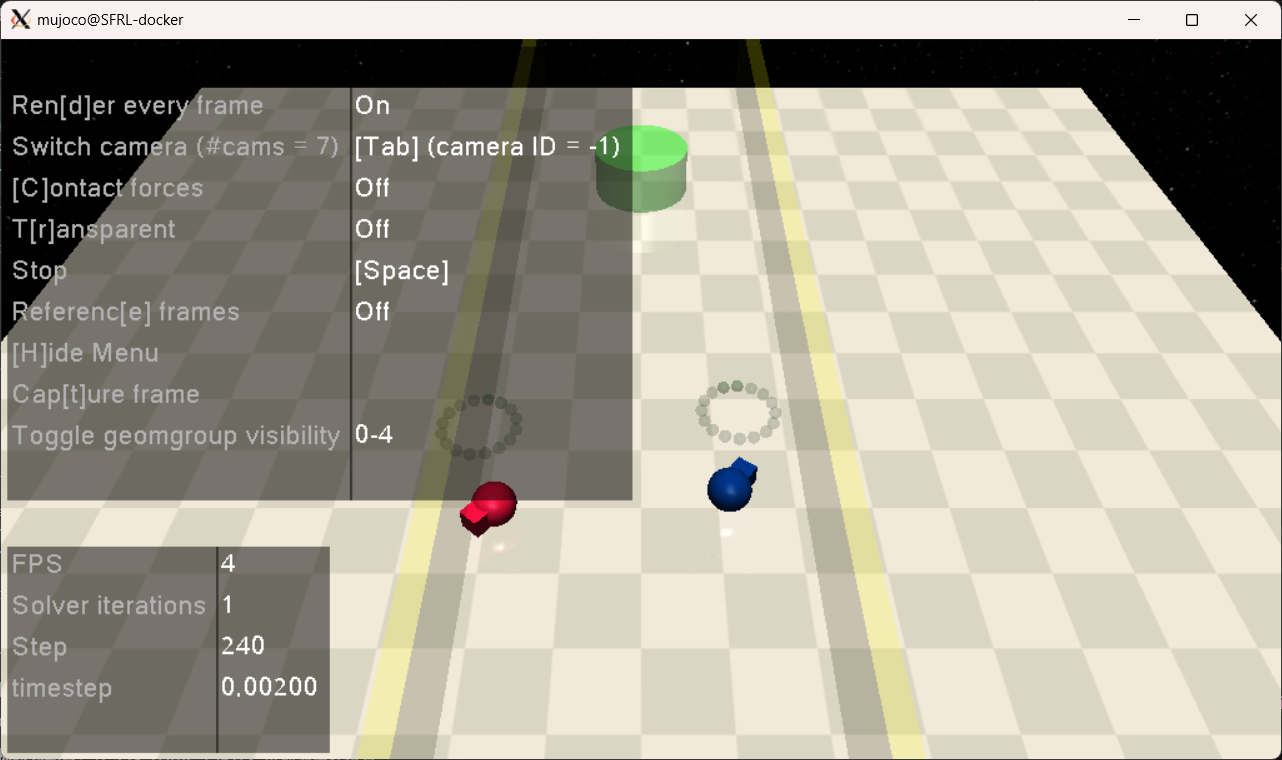
\includegraphics[width=1\linewidth]{images/rmp_env.png}
    \caption{Enter Caption}
    \label{fig:rmp_env}
\end{figure}

\subsection{评价指标}
为了全面评估算法性能，本文采用以下指标：
1）累计奖励（Total Reward）
统计策略在一个完整 episode 中获得的累计奖励：$R = \sum_t r_t$，反映策略整体行为质量。
2）安全代价（Collision Cost）
统计策略在一个完整 episode 中产生的累计安全代价：$C = \sum_t c_t$，用于评估系统安全性。
3）任务成功率（Success Rate）
成功率定义为：
\[SR = \frac{N_{success}}{N_{total}}\]
其中：$N_{success}$ 为成功到达目标且未发生碰撞的 episode 数；$N_{total}$ 为总测试 episode 数，该指标反映策略在复杂环境中的任务完成能力。

\subsubsection{奖励设置}
强化学习部分主要负责提供目标驱动和整体行为优化能力，因此设计了一系列奖励函数以引导策略学习合理的导航行为。
总奖励由多个子奖励组成：
\[r_t = r_{goal} + r_{progress} + r_{form} + r_{collision}\]
其中各部分定义如下。

\paragraph{目标导航奖励}
为了鼓励机器人不断接近目标位置，引入距离递减奖励：
\[r_{progress} = \beta (D_{last} - D_{now})\]
其中$D_{last}$为上一时刻机器人编队质心到目标的距离；$D_{now}$为当前时刻机器人编队质心到目标的距离；$\beta$为奖励权重系数。
当机器人朝目标移动时奖励为正；反之则为负，从而引导策略持续接近目标。
当机器人编队成功到达目标区域时，给予一次性的奖励：$r_{goal} = R_{goal}$，该奖励用于强化成功完成任务的行为。

\paragraph{编队保持奖励}
为保证多机器人系统在运动过程中维持期望的空间结构，本文设计如下编队保持奖励函数。设系统中共有 N 个机器人，其在二维平面中的位置为
\[
p = (p_0, p_1, \ldots, p_{N-1}), \quad p_i \in \mathbb{R}^2.
\]

当前编队形状由无向图 $\mathcal{G}=(\mathcal{V},\mathcal{E})$ 描述，其中每条边 $(i,j)\in\mathcal{E}$ 表示机器人 i 与机器人 j 之间需要保持期望距离 $d_{ij}^*$。该图结构与 GCPL 中用于构建编队保持节点的拓扑保持一致。

\subparagraph{距离保持奖励项}
对于任意约束边 $(i,j)$，定义其距离误差为
\[
e_{ij} = \left| |p_i - p_j|_2 - d_{ij}^* \right|.
\]

为了消除编队规模变化对奖励幅值的影响，采用所有边误差的平均值作为整体距离偏差：
\[
\bar{e} =
\begin{cases}
\frac{1}{|\mathcal{E}|} \displaystyle\sum_{(i,j)\in\mathcal{E}} e_{ij}, & |\mathcal{E}| > 0, \\
0, & |\mathcal{E}| = 0.
\end{cases}
\]

基于该平均误差，编队距离奖励定义为
\[
r_{\mathrm{dist}} = s_f \exp\left(-\frac{\bar{e}}{\tau}\right),
\]
其中 $s_f>0$ 为编队奖励尺度系数，$\tau>0$ 为距离容差参数，用于控制奖励对误差变化的敏感程度。当机器人间距离接近期望值时，$\bar{e}$ 较小，对应的奖励接近 $s_f$；而当编队结构被破坏时，奖励将随误差增大而快速衰减。

\subparagraph{形状辅助奖励项}

在部分编队形状中，仅依赖距离约束可能无法唯一确定整体朝向或宽度结构。为此，针对特定形状设计了额外的辅助奖励项 $r_{\mathrm{aux}}$。

在全连接网格（mesh）编队中，为避免结构发生整体旋转或镜像，引入边方向与期望方向的一致性奖励。对于边 ((i,j))，定义其单位方向向量为
\[
\hat{r}_{ij} = \frac{p_j - p_i}{|p_j - p_i|_2}.
\]

设 $\hat{r}^*$ 为期望的全局编队方向，则辅助奖励定义为
\[
r_{\mathrm{aux}} =
s_m \cdot
\frac{1}{|\mathcal{E}|}
\sum_{(i,j)\in\mathcal{E}}
\hat{r}_{ij}^\top \hat{r}^*,
\]
其中 $s_m>0$ 为方向一致性奖励权重。当编队边方向与期望方向对齐时，该项取得较高值，从而抑制编队在训练过程中发生无意义的旋转。

对于队列（line）编队，主要目标是保持机器人在某一主轴方向上排列，同时限制垂直方向的扩散。设编队主轴为 x 轴时，定义辅助奖励为
\[
r_{\mathrm{aux}} = - s_\ell , \mathrm{Var}( {p_{k,y}}),
\]
其中 $\mathrm{Var}(\cdot)$ 表示样本方差，$s*\ell>0$ 为宽度惩罚权重。该项通过惩罚机器人在垂直方向上的位置方差，使系统收敛到窄带状队列结构。若主轴为 y 轴，则对 x 坐标方差进行惩罚。

对于楔形（wedge）与圆形（circle）编队，其几何结构已由距离约束图 $\mathcal{E}$ 与目标距离 $d_{ij}^*$ 唯一确定，因此不额外引入辅助奖励项：
\[
r_{\mathrm{aux}} = 0.
\]

因此在每个时间步，对所有机器人采用共享的编队奖励信号：
\[
r_{\mathrm{form}}^k = r_{\mathrm{dist}} + r_{\mathrm{aux}},
\quad k = 0, \ldots, N-1.
\]

这种全局共享奖励设计与 MAPPO 的集中式训练机制相匹配，使各个智能体在优化自身策略时能够考虑整体编队结构的变化，从而学习到协同一致的群体行为。

\paragraph{碰撞惩罚}

如果机器人发生碰撞，则给予较大的负奖励：$r_{collision} = R_{collision}$。
该奖励用于强烈惩罚危险行为，促使策略避免碰撞。

\subsubsection{代价设置}

除奖励函数外，本文设计代价函数（Cost），用于度量系统在运行过程中产生的风险程度。该 cost 主要用于安全评估以及策略约束分析。
总安全代价定义为：
\[c_t = c_{hazard} + c_{robot}\]

障碍物接近代价：当机器人靠近环境障碍物时，产生风险代价：
\[c_{hazard} = \gamma (R_{hazard} - D_{hazard})\]
当$D_{hazard} < R_{hazard}$时产生代价，其中：$D_{hazard}$ 为机器人到最近障碍物的距离；$R_{hazard}$为危险距离阈值； $\gamma$ 为权重系数。
该代价函数呈 Barrier 型结构，当机器人靠近障碍物时迅速增加，从而刻画安全风险。

机器人间碰撞代价：
为了避免机器人之间的碰撞，引入机器人间安全距离代价：
\[c_i^{col} = \sum_{j\in\mathcal N_i} \beta_c \phi \big( d_{safe} - \|x_i - x_j\| \big)\]
其中： $d_{safe}$ 为机器人间安全距离；$\beta_c$ 为代价权重； $\phi(\cdot)$ 为ReLU 或 barrier 函数。
当机器人距离小于安全距离时，代价增加，从而反映系统风险。

\subsection{参数设置}
\begin{table}[htbp]
\centering
\small
\setlength{\tabcolsep}{6pt}
\renewcommand{\arraystretch}{1.2}
\begin{tabular}{p{0.22\linewidth} p{0.2\linewidth}|p{0.22\linewidth} p{0.2\linewidth}}
\hline
\multicolumn{2}{c|}{\textbf{训练参数}} & \multicolumn{2}{c}{\textbf{GCPL参数}} \\
\hline
\textbf{参数} & \textbf{参数大小} & \textbf{参数} & \textbf{参数大小} \\
\hline
总环境步数 & $10^8$ & 编队目标间距 & 0.5 \\
隐层宽度 & 512 &  直线编队轴向 & x \\
MLP层数 & 2 & 楔形半角（度） & 35.0 \\
折扣因子 & 0.96 & 期望编队方向 & [0.0, 1.0] \\
GAE系数$\lambda$ & 0.95 & 方向叶$\alpha_\theta$ & 1.0 \\
PPO裁剪系数 & 0.2 & 方向叶$\eta_\theta$ & 2.0 \\
mini-batch数量 & 1  & 方向叶度量$c_\theta$ & 10.0 \\
策略学习率 & $9\times10^{-5}$ & 碰撞安全半径 & 0.3 \\
价值学习率 & $5\times10^{-3}$ & 融合权重 & 1 \\

\hline
\end{tabular}
\caption{训练参数与GCPL参数}
\label{tab:train-rmp-cn}
\end{table}

\subsection{实验结果}
实验结果如图 ~\ref{fig:rmp_result}所示，可以看到在训练过程中，相比于 MAPPO，添加 GCPL 的方法 cost 明显降低，意味着机器人碰撞次数明显下降，安全性更好；同时reward 明显提升，在任务中表现更加出色。
同时，我们对训练结果进行了评估，分别用 MAPPO、MAPPO\_Lag 和我们的方法完成 20 轮次的任务，结果同样显示出我们的方法 reward 更高和 cost 更低，同时在20次任务中成功率更高。
\begin{figure*}[t]
\centering
\subfloat[reward]{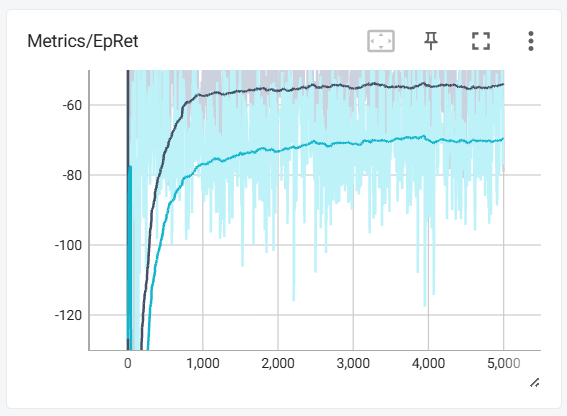
\includegraphics[height=4cm]{images/rmp_reward.png}}
\hfill
\subfloat[cost]{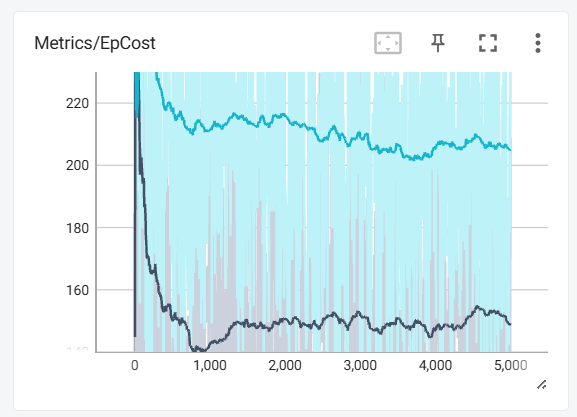
\includegraphics[height=4cm]{images/rmp_cost.png}}
\caption{GCPL 实验验证。其中蓝色表示mappo算法下的实验结果，黑色表示添加 GCPL 后的实验结果。(a) 训练过程中的reward (b) 训练过程产生的cost（表示碰撞次数）。}
\label{fig:rmp_result}
\end{figure*}

\begin{table}[htbp]
    \centering
    \caption{Experimental Results on SafetyPointMultiFormationGoal0-v0}
    \begin{tabular}{l c c c}
    \hline
    \textbf{Algorithm} & \textbf{Reward} & \textbf{Cost} & \textbf{Success Rate} \\
    \hline
    
    MAPPO      & $-21.46 \pm 3.43$ & $124.17 \pm 32.17$ & $0.13 \pm 0.09$ \\
    
    RMPflow  & $3.71 \pm 6.24$   & $22.85 \pm 19.37$  & $0.35 \pm 0.11$ \\
    
    MAPPO-Lag  & $-13.26 \pm 6.17$ & $125.96 \pm 34.05$ & $0.27 \pm 0.06$ \\

    GCPL  & $7.83 \pm 8.76$   & $27.15 \pm 14.51$  & $0.65 \pm 0.16$ \\
    
    \hline
    \end{tabular}
    \end{table}
\chapter{机器人安全验证平台}
强化学习方法在机器人控制任务中表现出良好的决策能力，但其在实际部署过程中仍面临显著的 sim-to-real gap 问题，尤其是在安全约束严格的应用场景中，策略在仿真环境中的有效性难以直接迁移到真实机器人系统。
另一方面，现有强化学习算法通常依赖于高并行度的训练环境以提升样本效率，而主流机器人仿真平台（如 Gazebo 和 Webots）在设计上更侧重于物理仿真与单实例交互，难以直接支持大规模并行训练。
因此，构建一个具备安全性验证能力且易于迁移至真实系统的中间验证平台具有重要意义。

基于上述背景，本文设计并实现了一套支持远程访问的机器人仿真验证平台。该平台通过浏览器端提供统一的实验入口，用户无需在本地部署复杂的机器人软件环境，即可远程访问仿真系统并执行算法验证任务。

% 对于RoboticsAcademy的改进：支持webots、支持多机器人实验、添加编队实验场景

\section{平台层次架构}

为支持安全强化学习算法在机器人系统中的高效验证，本文设计了面向仿真与真实系统统一的分层架构。该架构以模块解耦与接口标准化为核心原则，通过多层协同实现从算法开发到仿真验证再到系统部署的完整流程。平台总体结构如图~\ref{fig:platform_framework}所示，主要包括仿真与硬件层、中间件层、容器化后端层、应用与接口层以及前端交互层。

\textbf{（1）仿真与硬件层}作为系统的基础支撑层，负责构建机器人运行环境并提供物理交互基础。在仿真层面，平台基于 Gazebo 与 Webots 构建高保真机器人仿真环境，用于模拟多种机器人模型及复杂场景；在硬件层面，该结构可无缝扩展至真实机器人系统，从而支持算法的实际部署与验证。

\textbf{（2）中间件层}负责系统各模块之间的数据通信与功能解耦。平台采用 ROS 2 作为核心通信中间件，通过话题发布/订阅机制实现机器人状态信息（如位姿、速度与传感器数据）的实时传输，并支持控制指令的高效下发。同时，ROS 2 的分布式架构为多机器人系统提供了天然支持，使平台能够扩展至多智能体协同任务场景。

\textbf{（3）容器化后端层}用于实现系统运行环境的统一封装与调度管理。平台基于 Docker 构建容器化运行环境，将仿真系统、ROS 2 中间件以及算法模块集成于独立容器中。通过容器化部署，不同实验任务可在隔离环境中独立运行，从而保证实验结果的可复现性，并支持多场景并行执行与动态调度。

\textbf{（4）应用与接口层}是安全强化学习算法的执行核心。该层通过硬件抽象接口（HAL）对底层通信机制进行封装，使算法开发者能够以统一接口获取传感器数据并发送控制指令。同时，该层集成控制执行框架，实现感知、状态估计、策略计算与控制输出的闭环流程，并提供可视化接口以支持算法调试与结果分析。

\textbf{（5）前端交互层}作为系统的用户交互入口，实现远程访问与实验管理功能。用户无需在本地部署复杂环境，即可通过前端界面完成代码编写、仿真控制与运行监控。前端通过 WebSocket 与后端建立实时通信连接，实现机器人状态数据的动态更新与控制指令的低延迟传输。

通过上述分层架构设计，平台实现了机器人系统各功能模块之间的解耦与协同。该架构不仅提升了系统的可扩展性与可维护性，也为安全强化学习算法的系统化验证提供了稳定可靠的实验基础。

\begin{figure}
    \centering
    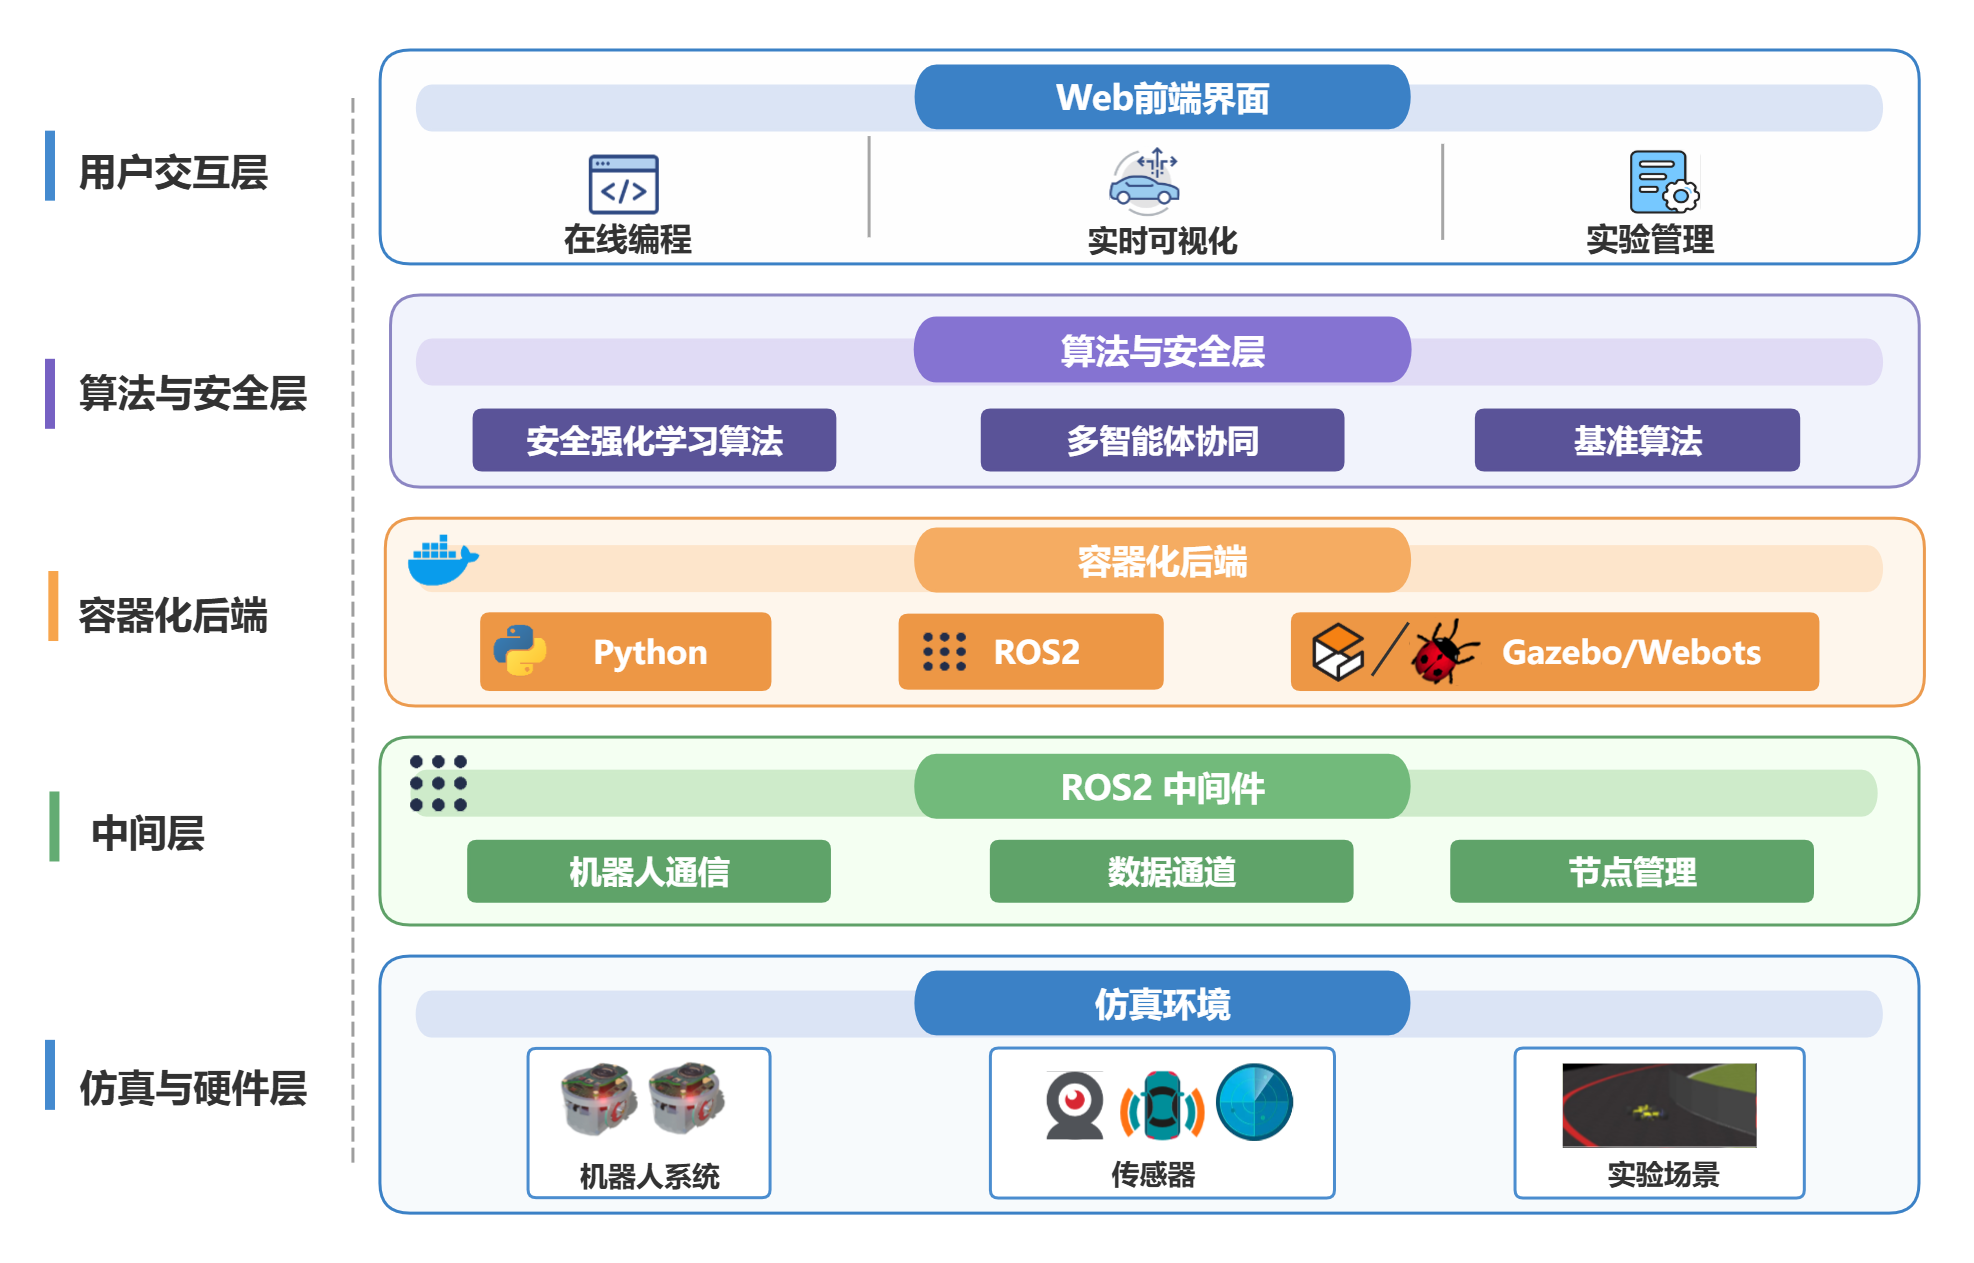
\includegraphics[width=1\linewidth]{images/platform_framework.png}
    \caption{Enter Caption}
    \label{fig:platform_framework}
\end{figure}

\section{核心机制设计}

在上述分层架构基础上，为提升平台在安全强化学习场景下的易用性，本文围绕实验可复现性、系统可解释性以及交互实时性，设计了三项关键机制：容器化并行调度机制、双通道可视化机制以及基于 WebSocket 的实时通信机制，从而提升平台性能与用户体验。

\subsection{容器化与并行调度机制}

针对强化学习算法对高并行训练环境的需求，以及机器人仿真环境在部署与依赖管理方面的复杂性，平台采用基于 Docker 的容器化运行机制对实验环境进行统一封装。

容器化运行机制中，每个实验任务均运行于独立的容器实例中，容器内部集成仿真引擎（如 Gazebo、Webots）、ROS 2 中间件以及算法执行模块。该设计使不同实验之间在软件依赖、运行状态及资源使用上实现完全隔离，从而避免环境冲突问题。同时，容器镜像在构建阶段已固定所有依赖版本，确保实验在不同时间与不同设备上的一致性，从而提升实验结果的可复现性。

在此基础上，平台通过容器调度机制支持多实例并行运行。后端系统根据用户请求动态创建、启动或销毁容器，实现实验任务的按需分配与资源管理。该机制不仅能够支持多用户并发访问，还可为强化学习算法提供并行环境，从而提升样本采集效率与训练速度。

\subsection{双通道可视化机制}

为提升机器人系统运行状态的可解释性与调试效率，平台设计了一种融合语义级状态表达与原生仿真界面展示的双通道可视化机制。

语义级可视化通道（WebGUI）从仿真环境中提取机器人位姿、传感器读数以及安全约束等关键状态信息，并将其统一组织为结构化数据，通过 WebSocket 实时推送至前端。前端采用组件化渲染方式，将上述数据映射为轨迹曲线、激光扫描、力向量以及约束边界等二维或抽象图形，从而直观呈现算法的内部状态与决策过程，使系统运行逻辑具备更强的可分析性与可解释性。

原生界面可视化通道（noVNC）则对仿真软件（如 Gazebo、RViz 或 Webots）的图形界面进行远程转发。后端依托虚拟显示技术启动图形化进程，并通过 VNC 协议将渲染结果实时传输至浏览器端，再以嵌入式页面形式进行呈现，从而完整保留原生仿真工具的交互能力与视觉效果，使用户能够获得与本地运行一致的使用体验。

该可视化机制通过语义层表达与原生图形复现的协同设计，同时支持对算法状态的细粒度分析与对仿真场景的完整观测，从不同维度增强系统整体的可视化表达能力。

\subsection{安全评估验证机制}
针对安全强化学习研究中实验结果难以复现、不同方法之间缺乏统一评估标准的问题，平台设计了一种统一的安全评估与模型验证机制，用于对不同算法在一致条件下进行系统性比较。

该机制首先对实验环境与任务配置进行标准化描述，包括机器人模型、场景结构、障碍物分布以及传感器参数等信息。所有算法均在相同环境配置下运行，从而消除外部因素对实验结果的影响。在此基础上，平台定义统一的评估指标体系，对算法性能进行多维度量化分析。

评估指标不仅包含传统强化学习中的任务完成率与累计奖励，还重点引入与安全相关的度量，例如约束违反次数、最小安全距离以及累计安全代价等。通过对安全性与任务性能的联合评估，可以更加全面地反映算法在复杂环境中的实际表现。

为支持已有模型的复现与对比，平台提供模型导入与验证接口。用户可以上传训练完成的策略模型文件，系统在加载模型后自动执行标准化验证流程，包括环境初始化、策略推理以及结果记录。该机制使不同来源的算法能够在统一平台上进行直接对比，避免因实现差异带来的评估偏差。


\section{系统实现}
为进一步明确系统功能组成与模块职责，本文从功能实现角度将平台划分为机器人仿真模块、前端交互模块、后端服务模块以及机器人通信模块四个核心模块。本节对平台各核心模块的具体实现进行说明。

\subsection{机器人仿真模块}
机器人仿真模块负责构建算法运行环境，并为控制策略提供可控且可复现的实验条件。系统采用 Docker 对仿真环境进行容器化封装，每个实验任务对应独立容器实例。容器内部集成仿真引擎、ROS 2 中间件及算法运行依赖，从而实现运行环境隔离，避免依赖冲突问题。
当用户启动某个实验任务时，系统会自动创建并启动对应的仿真容器，从而完成实验环境的初始化。

系统仿真引擎选用 Gazebo 与 Webots，两者均具备高保真物理建模能力以及丰富的机器人模型与传感器支持。通过配置文件描述实验场景，包括机器人结构、环境地图及障碍物分布，系统可按任务需求动态加载对应仿真环境，保证实验条件一致性。
用户编写的机器人控制程序在仿真环境中运行，获取机器人状态信息，并向机器人执行器发送控制指令，从而实现完整的机器人控制闭环。

ROS 2 节点负责连接仿真环境与算法模块。仿真器通过接口桥接发布机器人状态信息，包括位姿、速度及激光或视觉传感器数据；控制节点订阅相关话题并输出控制指令，形成闭环控制流程。所有话题名称与消息类型通过配置文件统一定义，从而保证不同任务之间接口一致。

图形界面通过虚拟显示机制提供。容器内部启动 Xvfb 或 Xvnc 构建虚拟显示环境，仿真程序在该显示环境中运行。VNC 服务将图像帧编码后通过网络传输至前端浏览器，实现远程渲染。用户可以通过浏览器实时查看机器人在环境中的运动状态，并根据实验结果对控制算法进行调整。

仿真模块周期性输出运行数据，包括机器人状态、传感器信息及控制量，并通过通信模块发送至前端，为状态可视化与算法分析提供数据支持。

本文通过容器化部署与仿真平台集成，构建了一个稳定、可扩展的机器人仿真环境，为机器人算法提供真实感较高的仿真测试场景，并保证实验环境的一致性与可复现性，为多机器人强化学习算法的实验验证提供了可靠的平台支持。

\subsection{前端交互模块}

前端交互模块基于单页应用（SPA）架构实现，采用 React 与 TypeScript 构建组件化界面。系统通过统一状态管理与路由机制组织各功能模块，从而提升整体可维护性与扩展能力。

\subsubsection{任务管理界面}

任务管理界面模块用于展示平台中可用的机器人实验任务，并提供实验任务的选择与管理功能。如图~\ref{fig:tasks}所示，用户可以通过该界面浏览平台中的实验场景列表，并查看每个任务的基本信息，例如任务名称、任务描述以及运行状态。

当用户选择某个实验任务时，前端系统会向后端服务器发送请求，获取对应任务的配置数据，并加载相应的仿真环境和界面组件。
\begin{figure}
    \centering
    
\includegraphics[width=1\linewidth]{images/tasks.png}
    \caption{任务管理界面}
    \label{fig:tasks}
\end{figure}

\subsubsection{任务运行界面}
任务运行界面通过向用户提供在线代码编辑器、任务控制面板以及仿真可视化窗口，使用户能够在浏览器环境中完成机器人算法的编写、运行与调试。如图~\ref{fig:follow_line}所示，页面左侧为代码编辑区，右侧为仿真可视化区及终端调试区，右上方任务控制面板用于管理实验流程与系统运行状态。
\begin{figure}
    \centering
    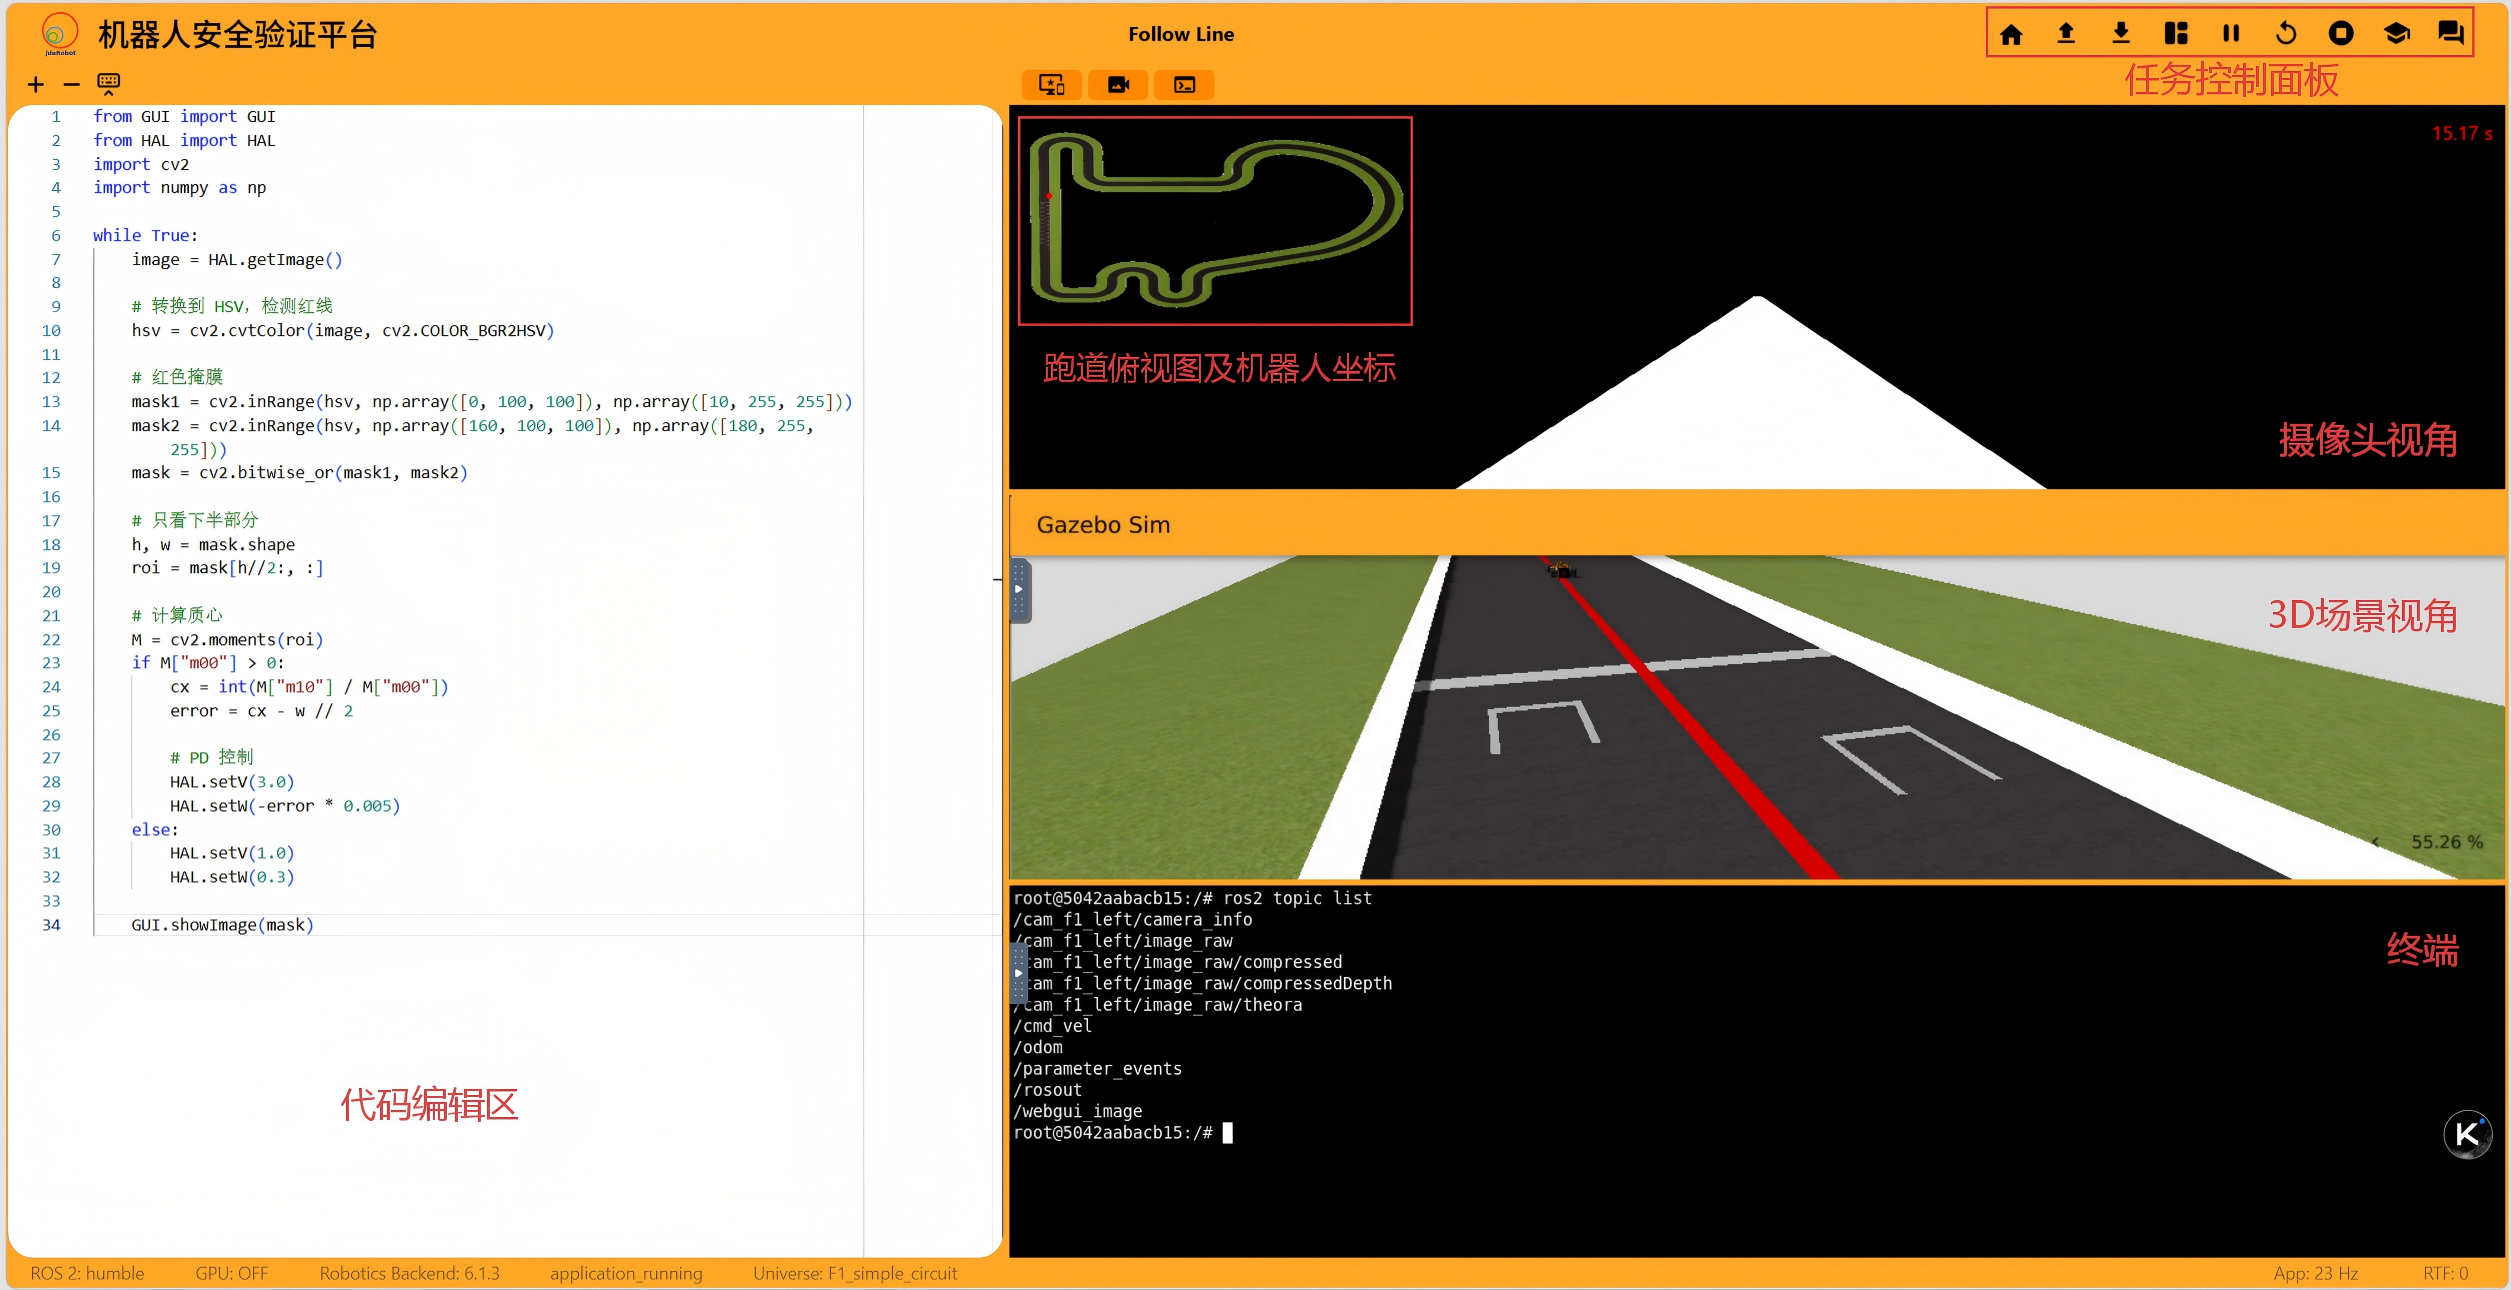
\includegraphics[width=1\linewidth]{images/follow_line(1).png}
    \caption{实验界面}
    \label{fig:follow_line}
\end{figure}

\paragraph{代码编辑区}
代码编辑区通过集成 IDE 组件实现代码编辑功能。
该模块支持在线代码编辑，并提供语法高亮、代码自动补全等功能，提高代码编写效率。同时系统允许用户选择不同的仿真环境或机器人模型配置实验环境。用户通过界面按钮可以启动、暂停或重新运行机器人程序。此外，系统支持代码文件的加载、保存以及模板文件下载。通过上述功能，系统为用户提供了类似本地开发环境的在线编程体验，使机器人算法开发过程更加便捷。

\paragraph{可视化展示区}
可视化展示区主要用于展示机器人仿真环境以及实验运行状态。该模块通过用组件级数据可视化（WebGUI）与桌面级远程可视化（noVNC）并行的方式进行实现。
数据可视化通过接收后端周期性推送的状态数据，并映射为二维图形，从而实现对系统状态的语义化表达。事件驱动触发局部组件更新的机制减少了不必要的重绘，提高了渲染效率。
远程桌面通过 Xvnc 与 noVNC 将图形界面以远程帧缓冲形式传输至浏览器，前端通过 iframe 加载对应页面，实现对 Gazebo、Webots 等原生界面的无侵入式展示。
此外，系统通过状态机驱动可视化组件的加载与显示，并支持多面板动态编排。

\paragraph{终端调试区}
终端调试区提供对后端运行环境的直接访问能力，支持实时查看程序执行过程中的标准输出与错误信息，从而辅助系统状态分析与问题定位。该功能通过远程终端机制进行实现。前端基于 noVNC 将容器内的 xterm 图形终端嵌入浏览器页面，实现终端界面的可视化展示。后端在虚拟显示环境中启动 Xvnc 服务与 xterm 进程，构建完整的终端会话，并通过端口映射建立浏览器与容器之间的访问通道。程序运行过程中产生的日志与输出信息通过伪终端（PTY）写入终端设备，由 xterm 解析并更新显示内容，随后经 VNC 协议传输至前端界面。该机制实现了浏览器端对容器内部终端环境的实时访问，保证了调试过程的连续性与交互性。

\subsection{后端服务模块}

后端服务模块基于 Django 框架构建，负责系统业务逻辑处理与资源管理。系统采用 RESTful 架构设计，通过统一 API 向前端提供数据访问接口，实现前后端解耦。

从功能结构上看，后端系统主要承担实验任务管理、API 服务提供、数据库管理以及系统调度与控制几个方面的功能。

\subsubsection{实验任务管理}
实验任务管理模块维护平台中的任务及其配置数据。每个任务包含机器人模型、仿真场景及算法模板等信息。系统根据任务标识读取配置并返回前端，用于初始化仿真环境。

实验任务管理模块负责维护平台中的机器人实验任务及其相关配置。每个实验任务均包含完整的环境描述信息，包括机器人模型、仿真场景、实验工具以及算法模板等。系统通过统一的数据结构对这些信息进行组织和管理，从而使不同实验任务能够在平台中进行统一调度。

当用户在前端界面选择某个实验任务时，后端系统会根据任务标识从数据库中读取对应的配置信息，并返回给前端系统。随后前端根据任务配置加载对应的仿真环境与界面组件，从而完成实验任务的初始化过程。

\subsubsection{API 服务提供}
为了实现前端系统与后端系统之间的数据交互，平台设计了一组 REST API 接口，用于向前端提供统一的数据访问服务。主要接口包括实验任务列表获取、实验配置加载以及代码模板下载等功能。

在系统运行过程中，前端应用通过 HTTP 请求调用相应的 API 接口。例如，当用户进入实验页面时，前端首先调用获取实验列表接口，从后端服务器加载所有可用实验任务；当用户选择具体任务时，系统再调用实验配置接口获取对应的仿真环境信息。这种基于 REST API 的通信方式能够有效降低系统耦合度，并提高系统的可扩展性。

\subsubsection{数据库管理}

为了实现平台资源的统一管理，系统采用 PostgreSQL 作为后台数据库，用于存储实验任务、仿真环境配置以及机器人模型等核心数据对象。PostgreSQL 具有良好的稳定性与扩展能力，能够支持复杂数据结构的存储与查询，适合用于机器人实验平台的数据管理。
在数据库设计方面，平台主要包含以下几个核心数据对象：
\begin{itemize}
    \item Task：具体的机器人实验任务；
    \item Universe：实验任务对应的仿真环境配置；
    \item World：定义具体的仿真场景；
    \item Robot：机器人模型及其控制接口；
    \item Tool：实验过程中使用的辅助工具组件。
\end{itemize}

通过上述数据结构，平台能够对不同机器人实验任务进行统一管理，并支持多种仿真环境配置。同时，Django 提供的对象关系映射（ORM）机制使得开发人员可以通过 Python 对象直接访问数据库，从而简化数据库操作并提高开发效率。

\subsubsection{系统调度与控制}
系统调度模块负责实验任务的生命周期管理。用户触发实验请求后，后端根据配置启动对应容器，并建立通信连接。同时维护运行状态，包括启动、暂停与终止等操作，保证任务执行过程的有序性与稳定性。

通过上述模块设计，后端服务系统实现了机器人实验任务管理、数据服务以及仿真调度等核心功能，为平台提供了稳定可靠的运行基础。同时，基于 RESTful 架构与模块化设计思想，系统具有良好的可扩展性，可以方便地接入新的机器人实验任务与仿真环境，从而满足多机器人强化学习研究的需求。

\subsection{机器人通信模块}
通信模块承担前端、后端与仿真环境之间的数据交互功能。由于机器人实验过程中需要频繁交换状态信息与控制数据，因此需要一种低延迟、高实时性的通信机制来保证数据传输效率。系统采用 WebSocket 建立持久连接，实现低延迟双向通信。

连接建立阶段，前端在实验启动时向后端发起请求，后端创建独立通信会话并返回连接确认信息。连接建立后，系统进入持续数据交互状态。

数据传输的信息包含仿真环境周期性生成的状态数据（如机器人位姿、传感器信息及系统运行状态），和用户触发的控制指令，包括程序执行控制与动作输入。状态数据由后端转发至前端进行实时更新，控制指令则传递至仿真系统完成执行。系统数据链路图如图~\ref{fig:data}所示。

通信模块同时负责运行状态同步与异常反馈。当仿真环境状态发生变化或出现错误时，相关信息将及时传输至前端，从而保证系统状态一致性并提高调试效率。

该通信机制有效降低了数据传输延迟，提升了系统交互实时性，为机器人在线仿真与安全策略验证提供了稳定的数据通道。
\begin{figure}
    \centering
    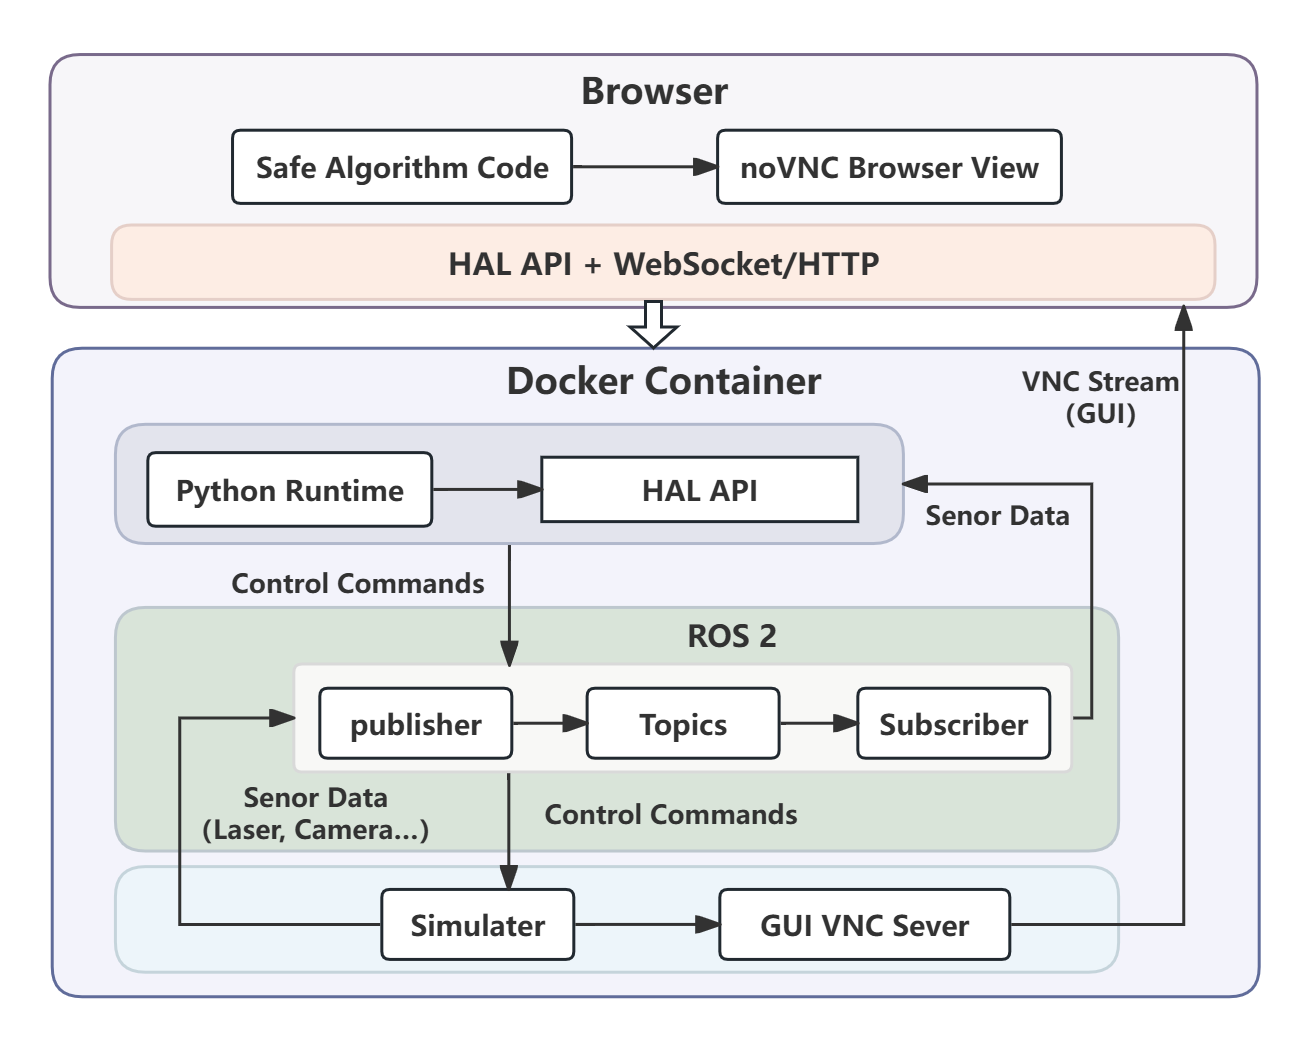
\includegraphics[width=1\linewidth]{images/platform data stream.png}
    \caption{系统数据链路图}
    \label{fig:data}
\end{figure}
\section{本章小结}

本章围绕安全强化学习算法的验证需求，设计并实现了一套面向机器人系统的仿真验证平台。针对传统机器人仿真环境在可复现性、并行能力以及安全验证支持方面的不足，平台从体系结构与关键机制两个层面进行了系统设计。

在体系结构上，平台采用分层架构，将仿真环境、通信中间件、容器化运行环境、算法执行逻辑以及前端交互界面进行解耦，实现了系统功能的模块化组织与统一接口管理。在此基础上，进一步通过容器化技术构建标准化运行环境，使不同实验任务能够在隔离条件下稳定运行，并支持多实例并行调度。

在关键机制方面，平台设计了容器化并行调度机制、双通道可视化机制以及基于 WebSocket 的实时通信机制。其中，容器化机制保证了实验环境的一致性与可复现性；双通道可视化机制实现了机器人运行状态的语义表达与原生仿真展示的有机结合；实时通信机制则为系统提供了低延迟的数据交互能力，确保了仿真过程的实时性与交互性。

在具体实现上，系统完成了仿真模块、前端交互模块、后端服务模块以及通信模块的开发，构建了从任务管理、环境部署到运行监控的完整流程。通过统一的数据接口与调度机制，各模块之间实现了高效协同，能够稳定支持多场景、多任务的机器人算法验证。

本章所构建的机器人安全验证平台为后续安全强化学习算法的实验研究提供了统一、可扩展且具有良好可解释性的基础环境，为多机器人系统在复杂场景下的安全决策研究奠定了支撑。
   % 多机器人安全强化学习的容器化仿真验证平台 (input chap51.tex)
\chapter{结论与展望}

\section{结论}
本文研究不确定环境下机器人的安全强化学习问题，按"单体安全—群体协同—系统验证"三条线索展开：第3章解决单机器人执行层的硬安全保障，第4章把安全约束推广到多机器人编队的几何关系，第5章将两者集成到统一的容器化平台上进行验证。

第3章提出约束流形策略学习方法（CMPL）。其核心是把策略输出投影到安全可达空间的切空间，使动作在执行前即被修正到满足硬约束，而非依赖奖励惩罚的间接引导；状态估计则用一个由卷积神经网络学习观测噪声协方差的扩展卡尔曼滤波器，为安全过滤器提供更可靠的输入。在 Safety-Gymnasium 的目标到达任务中，CMPL 将平均安全代价从 PPO 基线的 50.58 降到 4.91（降幅 90.3\%）；在 Webots 的 E-puck 零样本部署中，碰撞率由 40\% 降至零，位置误差降低 27.5\%。

第4章针对多机器人编队中任务目标与安全约束相互耦合的问题，提出几何约束策略学习方法（GCPL）。该方法用 MAPPO 学习任务级控制意图，再由几何过滤层在黎曼流形上统一处理编队拓扑、机间安全距离与避障，并对动作做解析修正，把任务驱动与结构约束解耦到两层。在线形编队任务上，GCPL 相对 MAPPO 基线将安全代价从 105.78 降到 18.53，编队完成度由 10\% 提升到 71\%，成功率由 2\% 提升到 66\%；在楔形、圆形等更复杂拓扑上同样保持领先。

第5章面向方法验证与工程落地，设计并实现了一套容器化仿真验证平台：用分层架构和 Docker 镜像固化运行依赖，并提供统一的评估管线支持多算法在相同条件下的公平对比。平台把第3、4章方法按 MAPPO→GCPL→CMPL 的顺序串联，先在纯 Python 的 MVP 上验证控制链路的数学正确性，再迁移到 Webots 做四档消融。四档实验全程零碰撞，完整分层配置在编队一致性上最优（编队误差 0.082~m），到达率则随各模块权重组合在安全裕度与目标驱动之间权衡——这说明安全机制能在策略尚未收敛时提供保护，但任务完成度仍取决于策略本身的优化程度。

三部分工作由"在动作执行前于约束流形上显式修正安全约束"这一共同思想衔接：CMPL 给出单体硬安全，GCPL 把它推广到群体几何协调，平台则让二者在统一环境下端到端运行并可复现地对比。

\section{展望}

尽管本文在多机器人安全强化学习方面取得了一定进展，但仍存在若干值得进一步研究的问题，未来可从以下几个方向开展深入探索：

（1）本文方法主要依赖离线可达性分析与先验环境信息，在动态障碍物或未知环境中仍存在一定局限。未来可结合在线学习或自适应可达性分析方法，实现安全区域的动态更新，从而提升系统在强不确定环境中的适应能力。

（2）随着机器人数量的增加，多智能体系统在通信负载、计算复杂度和策略协同方面会面临更高要求。未来可结合图神经网络、分布式学习等方法，进一步提升算法在大规模系统中的扩展能力与计算效率。

（3）本文实验主要基于仿真环境完成，后续工作仍需在实际机器人平台上开展进一步实验，重点考察传感器误差、执行器延迟、通信不稳定和场景扰动等因素对方法性能的影响。

（4）本文提出的 GCPL 方法在常规编队导航任务中能够降低碰撞风险并提升队形稳定性，但在密集编队、狭窄通道等复杂场景中，固定权重或度量矩阵可能导致局部极小值、路径震荡等问题。后续可引入动态权重调整、任务优先级和冲突重规划机制，使编队能够根据环境变化临时调整形态，并在通过复杂区域后恢复目标队形。

（5）本文的数据驱动 EKF 主要基于速度相关的高斯噪声模型进行训练，能够刻画运动速度增大导致测量误差上升的情况。但真实环境中的噪声可能更加复杂。后续可进一步考虑非高斯噪声、突发异常和分布外场景，并结合异常检测、在线校准或不确定性估计，提高状态估计模块在真实环境中的稳定性。   % 结论与展望


\chapter*{参考文献}\addcontentsline{toc}{chapter}{参考文献}

\printbibliography[heading=none]


%% 附录
% \appendix

\chapter{单位}

以下内容可放在附录之内：
\begin{enumerate}
\item 正文内过于冗长的公式推导；
\item 方便他人阅读所需的辅助性数学工具或表格；
\item 重复性数据和图表；
\item 论文使用的主要符号的意义和单位；
\item 程序说明和程序全文；
\item 企业应用证明；
\item 项目鉴定报告；
\end{enumerate}
%% 致谢
%% 致谢
%\pagestyle{empty}
\chapter*{致\quad\quad 谢}\addcontentsline{toc}{chapter}{致谢}
% 行文至此，我的硕士生涯终将落笔收官。

% 三年的点滴片段仍在脑海中一帧帧闪现。谨以此段致谢，纪念属于我的一段漫长而充实的时光。

% 谢谢万老师为我提供学习成长的平台，谢谢段老师耐心细致地指导，让没有天赋的我完成了曾以为困难的事。老师们无论是学术还是精神品格，都深深影响了我。

% 谢谢笨笨熊和我一起讨论学术，一起克服困难，接住了我所有的坏情绪，为我带来很多欢乐，为我荒芜的世界添加很多色彩。

% 谢谢猪猪，我12年的挚友。好朋友是生活的解药。很幸运能相遇。我们一起经历了很多人生中重要的时刻。

% 谢谢家人，

% 谢谢朋友们，

% 感谢旅途上的曲折与遗憾;感谢迷茫与不安;

% 感谢自己。
% 在无数个夜晚煎熬，对未发生的事忧虑，对已发生的事懊悔。
% 逐渐发觉很多事情努力很重要、选择很重要，甚至运气很重要、性格很重要，
% 但无论结果如何，正是这诸多因素铸成了今天的我。
% 感谢这一路走的很慢却一直没有放弃的自己，愿你带着这份笨拙的坚持继续往前走，勇敢、积极、热烈!

% 未来的路还很长，我会带着这些年的收获与成长，带着所有人给我的爱与底气，继续往前走，永远记得这份赤诚与温暖，永远保有对真理的热爱、对生活的热忱。
行文至此，我的硕士生涯终将落笔收官。三年的求学时光漫长而充实，其中有困惑、有压力，也有成长与收获。回望这一路，许多人与事仍清晰地留在记忆里。谨以此段致谢，纪念这段珍贵的时光，也向所有曾给予我帮助、支持与温暖的人表达最诚挚的感谢。

首先，衷心感谢我的导师万老师。感谢您为我提供了学习和成长的平台，在科研方面给予我指导与支持。您的教诲让我逐渐明白，科研不仅需要扎实的专业能力，也需要持续的耐心、严谨的态度和面对问题时不断探索的勇气。
特别感谢段老师在我研究生阶段给予的悉心指导和关怀。从论文选题、方法设计，到实验分析和文字修改，您始终耐心地帮我梳理问题、完善思路，也在一次次讨论中教会我如何更严谨地对待学术。您对科研认真负责，对学生却始终温柔耐心，在我迷茫、焦虑或进展不顺利的时候，您给予了我很多理解和鼓励。很多次看到您周末仍在学校、深夜还在处理工作，我都深切感受到您对学术和学生的责任与投入。能够在研究生阶段得到您的指导和帮助，是我莫大的幸运。
老师们在学术上的严谨、在工作中的认真，以及在为人处世中的包容与善意，都对我产生了深远影响。

感谢笨笨熊一路以来的陪伴。谢谢你陪我讨论学术问题，陪我一起面对困难，也接住了我许多低落和崩溃的时刻。你为我带来了很多欢乐，也为我原本有些荒芜的世界增添了许多色彩。那些一起努力、一起焦虑、一起玩笑的日子，都是这段研究生生活中非常珍贵的记忆。

感谢猪猪，我十二年的挚友。好朋友是生活的解药。很幸运能够与你相遇，也很感谢我们一路陪伴彼此，见证了对方许多重要的人生时刻。无论距离远近，你的支持和理解一直是我心中稳定而温暖的力量。

感谢我的家人。谢谢你们在我成长过程中给予的爱、包容与支持。无论我身处何处、遇到怎样的困难，你们始终是我最坚实的后盾。你们不曾给我过多压力，却一直用自己的方式鼓励我向前走。正是这份无条件的爱，让我在疲惫和迷茫时仍有继续坚持的底气。

感谢一路同行的朋友们。谢谢你们在平凡的日子里给予我的陪伴、安慰和鼓励。那些聊天、散步、分享快乐与烦恼的时刻，让紧张的学习生活变得柔软而明亮。因为有你们，这三年不只有论文和实验，也有许多值得记住的温暖瞬间。

感谢这一路上的曲折、遗憾、迷茫与不安。它们曾让我焦虑，也让我成长。过去的许多个夜晚，我曾为尚未发生的事情担忧，也曾为已经发生的事情懊悔。后来我逐渐明白，人生中努力很重要，选择很重要，甚至运气很重要，性格很重要。但无论结果如何，正是这些经历共同塑造了今天的我。

最后，感谢那个走得很慢、时常怀疑，却始终没有真正放弃的自己。感谢自己在无数个想要退缩的时刻，仍然笨拙而认真地坚持了下来。愿未来的自己继续带着这份赤诚与勇气向前走，勇敢、积极、热烈，也永远保有对真理的热爱和对生活的热忱。

未来的路还很长。我会带着这些年的收获与成长，带着师长的教诲、朋友的陪伴和家人的爱与底气，继续坚定地走下去。愿我永远记得这份温暖，也永远珍惜这一路所得的一切。
%% 作者简历及在学研究成果
%% 作者简历及在学研究成果
\chapter*{作者简历及在学研究成果}\addcontentsline{toc}{chapter}{作者简历及在学研究成果}

\section*{一、主要教育经历/工作经历（从大学起，到硕士入学止）}


% ...
\noindent\begin{tabularx}{\textwidth}{|>{\centering\arraybackslash}X|>{\centering\arraybackslash}X|>{\centering\arraybackslash}X|}
  \hline
  起止年月 & 学习或工作单位 & 备注 \\\hline 
  2019年9月至2023年6月  & 在北京科技大学计算机科学与技术专业攻读学士学位  & X  \\\hline

  & & \\ \hline
\end{tabularx}

\section*{二、在学期间从事的科研工作}

% （1）高性能低功耗深度神经网络处理器芯片设计（USTB06500093），主要参与人员，2017.11-2022.11。

% （2）... 

\section*{三、在学期间所获的科研奖励}

（1）硕士研究生学业奖学金

\section*{四、在学期间发表的论文}

% [1] 	\textbf{Liu M. K.}, Liu C. X., Zhang S. T., et al. Research on Industry Development Path Planning of Resource-Rich Regions in China from the Perspective of “Resources, Assets, Capital” [J]. Sustainability, 2021, 13(7): 3988-3988.


% {\color{blue} 盲审说明（正式写作请删除此说明）：}

% 盲审论文需要隐藏掉所有会影响盲审结果的论文作者及其导师的信息，以便论文评
% 阅人能够公正的进行评阅。

% 当学校要求提供盲审论文时，请按如下方法制作。

% 1) 对于论文中下列学生和导师信息。请将学生姓名、学生学号、导师姓名，依次全
% 部替换为[本论文作者] 、[论文作者学号]、[本论文导师]。论文中上述信息均需要替换，
% 包括作者研究成果等部分的有关信息。

% 2) 在研究成果中，论文作者发表的文章列表中应隐去所有作者的名字，只标明论文
% 期刊名，级别，发表年份。

% 3）盲审论文，请不要填写致谢，致谢页除标题、页眉、页码外请保持空白。

% 4）其他会影响盲审结果的信息，请采用类似方式处理。

% 5）提交的盲审论文应为正式论文，除了上述替换后的信息外，应为可以评阅的正式
% 论文。

% 6）论文封面，请填写专业名称、论文题目等，将学号和姓名项目保持空白不填。制
% 作盲审论文时，论文书脊、封二、题名页请删除。

% 替换前后将文档分别保存，以便盲审论文与其他论文分开管理。

% {\color{blue} 盲审样例（正式写作请删除此样例）：}

% 五、在学期间发表的论文：

% [2] \textbf{第二作者（导师一作）}.中国矿业.中文核心期刊.2020.


\pagestyle{empty}
%% 关于论文使用授权的说明
\postDeclarations
%% 学位论文数据集
\chapter*{学位论文数据集}\addcontentsline{toc}{chapter}{学位论文数据集}
\vskip16.5pt
\noindent\zihao{5}\begin{tabu} to \textwidth{|X|X|X|X|X|}
\hline
关键词* & 密级* & 中图分类号* & UDC & 论文资助 \\\hline
约束流形；多智能体强化学习；多机器人编队；安全强化学习& 公开 & TP18 & & \\\hline
\multicolumn2{|l|}{学位授予单位名称*} & {学位授予单位代码*} & 学位类别* & 学位级别* \\\hline
\multicolumn{2}{|l|}{北京科技大学}&10008  & 学术型 & 硕士 \\\hline
\multicolumn2{|l}{论文题名*} & \multicolumn2{|l|}{并列题名} & 论文语种* \\\hline
\multicolumn4{|l|}{不确定环境下多机器人的强化学习安全策略研究} & 中文 \\\hline
作者姓名*&\multicolumn{2}{l|}{成孜卓} & 学号* & M202310641 \\\hline
\multicolumn2{|l|}{培养单位名称*} & 培养单位代码* & 培养单位地址 & 邮编 \\\hline
\multicolumn2{|l|}{北京科技大学} &10008 & 北京市海淀区学院路30号& 100083\\\hline
\multicolumn2{|l|}{学科专业*} & 研究方向* & 学制* & 学位授予年* \\\hline
\multicolumn2{|l|}{计算机科学与技术} & 安全多智能体强化学习 & 3年 & 2026年 \\\hline
论文提交日期* & \multicolumn4{l|}{2026年 06月 02日} \\\hline
导师姓名*&\multicolumn2{l|}{万亚东} & 职称* & 教授 \\\hline
评阅人 &答辩委员会主席* & \multicolumn3{l|}{答辩委员会成员} \\\hline
& 阿孜古丽 & \multicolumn3{l|}{} \\
& & \multicolumn3{l|}{} \\\hline
\multicolumn5{|l|}{电子版论文提交格式  文本（\, ）  图像（\, ） 视频（\, ） 音频（\, ） 多媒体（\, ） 其他（\, ）}\\
\multicolumn5{|l|}{推荐格式：application/msword; application/pdf} \\\hline
\multicolumn2{|l}{电子论文出版（发布）者} & \multicolumn2{|l|}{电子论文出版（发布）地} & 权限声明　\\\hline
\multicolumn2{|l}{} & \multicolumn2{|l|}{} & \\\hline
论文总页数* & \multicolumn4{l|}{80} \\\hline
\multicolumn5{|l|}{共33项，其中带*为必填数据，为22项。}\\\hline
\end{tabu}

\end{document}